\chapter{پیاده‌سازی و طراحی}
در این فصل، به چگونگی پیاده‌سازی پروژه و طریقه شکل‌گیری دوقلوی دیجیتال خیابان رشت می‌پردازیم.

\section{نگاهی به مسیر طی شده}
از آنجایی که این پروژه، پژوهشی بزرگ محسوب می‌شود، نیاز است تا فلوچارتی\LTRfootnote{\lr{Flowchart}} برای درک آن کشیده شود.

\begin{figure}[h!]
    \centering
    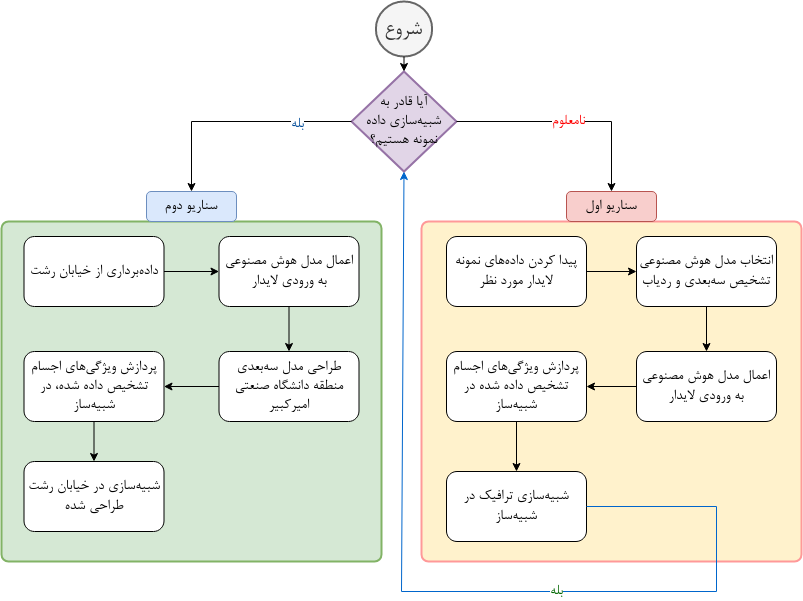
\includegraphics[width=1\linewidth]{figures/Project_Flowchart.png}
    \caption{فلوچارت پروژه}
    \label{fig:Project_Flowchart}
\end{figure}

همانطور که طبق \cref{fig:Project_Flowchart} مشاهده می‌شود، اولین سوالی که پیش‌ می‌آید، امکان‌پذیر بودن این پژوهش است.

\section{سناریو اول: استفاده از داده‌های نمونه}
گرفتن مجوز برای داده‌برداری از خیابان رشت و هماهنگی‌های لازم آن، هزینه‌بر است و تا زمانی که نتوان از امکان‌پذیر بودن این پژوهش اطمینان حاصل یافت، نمی‌توان آن را انجام داد. به همین دلیل، در ابتدا سناریو اول پیش گرفته شد که در آن، اقدام به شبیه‌سازی داده‌های نمونه موجود در تارنمای\LTRfootnote{\lr{Website}} شرکت \lr{Ouster} شده است.

\subsection{پیدا کردن داده‌های نمونه لایدارهای شرکت \lr{Ouster}}
تارنمای شرکت \lr{Ouster}، داده‌های نمونه‌ای را در اختیار توسعه‌دهندگان گذاشته است. یکی از این داده‌های نمونه، حسگر لایداری است که بر روی یک چراغ راهنمایی رانندگی، در یک چهارراه نصب شده است \LTRfootnote{\url{https://data.ouster.dev/\#/share/7LQRDQD3APIJL15L}}. 

\begin{figure}[h!]
    \centering
    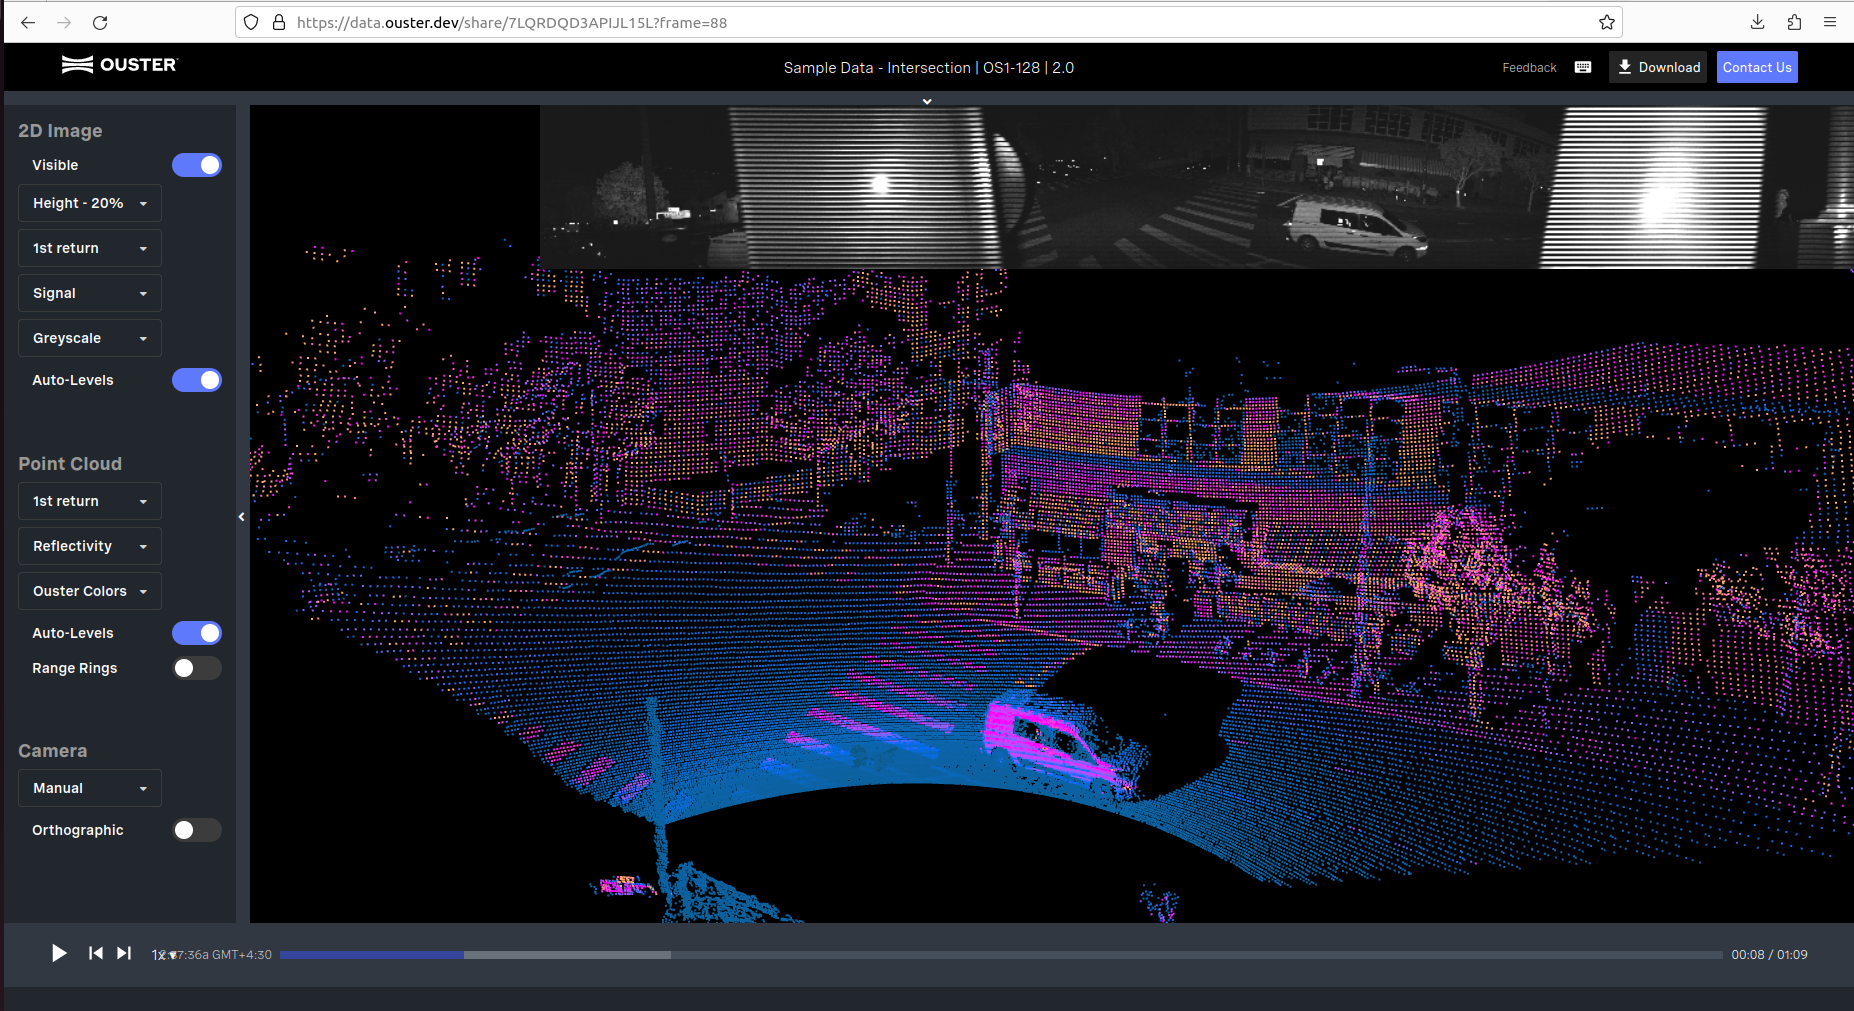
\includegraphics[width=1\linewidth]{figures/Ouster_Sample_Data_Intersection.png}
    \caption{داده‌ی نمونه که با لایدار \lr{OS1:128} ضبط شده است.}
    \label{fig:Ouster_Sample_Data_Intersection}
\end{figure}

با توجه به \cref{fig:Ouster_Sample_Data_Intersection}، مشاهده می‌شود که می‌توان داده‌‌ نمونه را بر روی کامپیوتر شخصی نیز دریافت کرد. داده‌های ابرنقاط عموما حجیم هستند و به طور مثال، داده فوق حدود ۲ گیگابایت\LTRfootnote{\lr{Gigabyte}} حجم دارد. 

\section{انتخاب مدل هوش مصنوعی تشخیص سه‌بعدی و ردیاب}
حال زمان آن رسیده است که مدل هوش مصنوعی‌ تشخیص دهنده‌ای را برای این پژوهش انتخاب کرد. در این پژوهش، تشخیص اجسام تنها با استفاده از ابر نقاط صورت می‌گیرد. از فصل مفاهیم پایه به یاد داریم که سه روش مختلف برای تشخیص اجسام سه‌بعدی استفاده می‌شود. عموما سرعت مدل‌های مبتنی بر واکسل، از دیگر روش‌ها بیشتر است و از آنجایی که در این پژوهش، داده‌های ورودی بلادرنگ هستند، بایستی سرعت مدل جدی گرفته شود. با جستجو و تحقیقات در مورد مدل‌های تشخیص اجسام سه بعدی، به چند مخزن\LTRfootnote{\lr{Repository}} و مقاله دست‌ یافته شده است.

\subsection{مدل \lr{SFA3D}}
این مخزن معروف، مدلی بسیار سریع است که از مجموعه داده \lr{KITTI} برای تمرین و آزمون استفاده می‌کند. 
\begin{figure}[h!]
    \centering
    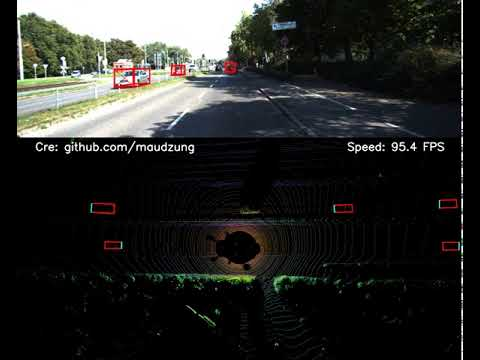
\includegraphics[width=0.75\linewidth]{SFA3D.png}
    \caption{تشخیص بلادرنگ مدل \lr{SFA3D}، با سرعت تشخیص بیشتر از ۹۰ فریم در ثانیه \cite{Super-Fast-Accurate-3D-Object-Detection-PyTorch}}
    \label{fig:SFA3D}
\end{figure}
در ابتدا این مدل ایده‌آل به نظر می‌رسید، اما مشکلاتی دارد که عبارتند از:
\begin{enumerate}
    \item این مدل از مجموعه داده \lr{KITTI} استفاده می‌کند که نسبت به دو مجموعه داده \lr{Waymo Open} و \lr{nuScenes}، بسیار ناقص‌تر است. این مدل بر روی مجموعه داده \lr{KITTI} خوب عمل می‌کند، اما در عمل با افت دقت روبرو خواهد شد.
    \item این مدل، سیستمی برای ردیابی و انتساب شناسه به اجسام ندارد.
    \item این مدل نسبتا قدیمی است و مدل‌های بهتر و قوی‌تری وجود دارند.
\end{enumerate}

\subsection{مخزن \lr{MMDetection3D}}
مخزن \lr{MMDetection3D}، یک جعبه‌ابزار متن‌باز برای تشخیص اجسام سه‌بعدی است. این مخزن توسط شرکت \lr{OpenMMLab}\LTRfootnote{\url{https://openmmlab.com/}} از کشور چین ساخته شده است، که جعبه‌ابزارهایی را در انواع زمینه‌های هوش مصنوعی، طراحی کرده است. کاربران با توجه به نیازمندی خود، می‌توانند به مخزن هر کدام از این جعبه‌ابزارها مراجعه کنند. این جعبه‌ابزارها بسترهایی هستند که با استفاده از آنها، کاربران می‌توانند مدل‌های دلخواه خود را انتخاب کنند و تنها با دریافت کردن مجموعه‌داده مورد نیاز، مدل انتخاب شده را آموزش دهند. به طور مثال، در مخزن \lr{MMDetection3D}، بیش از ۳۰۰ مدل مختلف پیاده‌سازی شده‌اند و مدل‌های جدید همواره در حال پیاده‌سازی و اضافه شدن به این مخزن هستند.

\begin{figure}
    \centering
    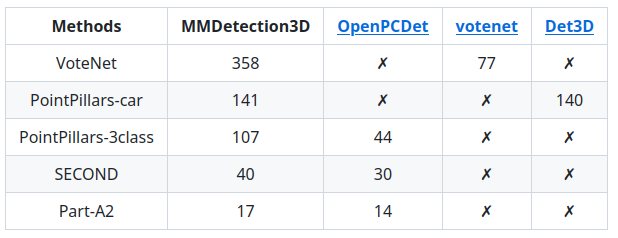
\includegraphics[width=0.75\linewidth]{figures/MMDetection3D_Models.png}
    \caption{تعداد مدل‌های پیاده‌سازی شده در مخزن \lr{MMDetection3D} \cite{mmdet3d2020}}
    \label{fig:MMDetection3D}
\end{figure}

طبق \cref{fig:MMDetection3D}، می‌توان مشاهده کرد که این مخزن در حال حاضر ۱۰۷ عدد مدل ابرنقاط محور مبتنی بر واکسل دارد و از معماری \lr{PointPillars} استفاده می‌کنند. یکی از مدل‌های معروف این مخزن، که در سال ۲۰۲۱ ساخته شد و همچنان از آن استفاده می‌شود، مدل \lr{CenterPoint}\cite{yin2021center} است.

\subsubsection{مدل تشخیص اجسام سه‌بعدی \lr{CenterPoint}}
اشیاء سه‌بعدی معمولاً به عنوان کادرهای محصور‌کننده سه‌بعدی در ابرنقاط نمایش داده می‌شوند. این نمایش، شبیه کشف کادر‌های محصورکننده دوبعدی بر پایه تصویر است، اما در فضای سه‌بعدی با مشکلاتی مواجه می‌شود. اشیاء در جهان سه‌بعدی هیچ جهت خاصی را دنبال نمی‌کنند و  مدل‌های مبتنی بر این کادرها، مشکلاتی در شمارش تمام جهت‌ها یا تلفیق یک کادر مرزی تطابقی به اشیاء چرخان دارند. اما در این مقاله، اشیاء سه‌بعدی به عنوان یک سری نقاط، نمایش، تشخیص و ردیابی می‌شوند. چهارچوب این مدل، \lr{CenterPoint}، ابتدا مراکز اشیاء را با استفاده از یک تشخیص‌دهنده نقاط کلیدی\LTRfootnote{\lr{Keypoint Detector}} یافته و سپس به ویژگی‌های دیگر از جمله اندازه سه‌بعدی، جهت سه‌بعدی و سرعت بازمی‌گرداند. در مرحله دوم، این تخمین‌ها را با استفاده از ویژگی‌های نقطه‌ای دیگر استنتاج شده از اجسام، بهبود می‌دهد. در مدل \lr{CenterPoint}، ردیابی اجسام سه‌بعدی با تطبیق حریصانه به نزدیک‌ترین نقطه\LTRfootnote{\lr{Greedy Closest-Point Matching}} ساده‌سازی می‌شود زیرا اجسام به نقاط معارف آن جسم تصویر شده‌اند. الگوریتم تشخیص و ردیابی حاصل، ساده، کارآمد و موثر است. \lr{CenterPoint} عملکرد برجسته‌ای را در آزمایش‌های آنلاین مجموعه داده \lr{nuScenes} در رده‌بندی‌های تشخیص و ردیابی سه‌بعدی، به ثبت رساند. این مدل با ۵.۶۵ امتیاز \lr{NDS} و ۸.۶۳ امتیاز \lr{AMOTA} برای یک مدل مبتنی بر ابر نقاط، به بهترین عملکرد ممکن در زمان خود رسید. این مدل در مجموعه داده  \lr{Waymo Open}، تمام روش‌های مدل تک‌مرحله‌ای قبلی را با اختلاف زیادی پیش‌می‌گیرد و در میان تمام مدل‌های مبتنی بر ابر نقاط، جایگاه اول را در سال ۲۰۲۱ گرفت \cite{yin2021center}.

\begin{figure}[h!]
    \centering
    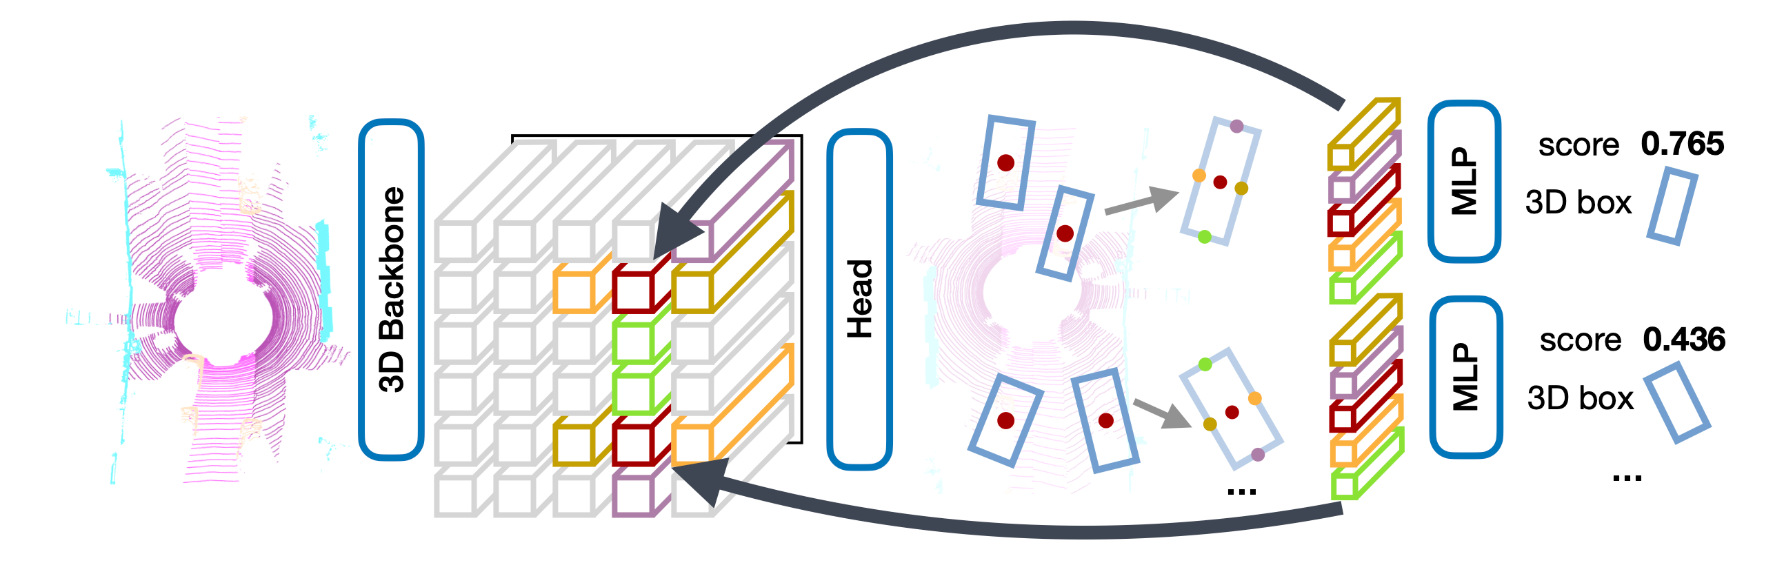
\includegraphics[width=1\linewidth]{figures/Centerpoint_Architecture.png}
    \caption{معماری مدل \lr{CenterPoint} \cite{yin2021center}}
    \label{fig:CenterPoint_Architecture}
\end{figure}

\begin{table}[h!]
    \centering
    \caption{جدول مقایسه مدل‌های سه‌بعدی براساس ارزیابی مجموعه داده \lr{Waymo Open} \cite{yin2021center}}
    \begin{tabular}{cccccc}
        \hline
        \multirow{2}{*}{\textbf{سختی}} & \multirow{2}{*}{\textbf{مدل}} & \multicolumn{2}{c}{\textbf{خودرو}} &\multicolumn{2}{c}{\textbf{عابر پیاده}}\\
        & & \lr{mAP} & \lr{mAPH} & \lr{mAP} & \lr{mAPH}\\
        \hline
        & \lr{StarNet} & 5.61 & 0.61 & 8.67 & 9.59 \\
        & \lr{PointPillars} & 3.63 & 8.62 & 1.62 & 2.50 \\
        \lr{Level 1} & \lr{PPBA} & 5.67 & 0.67 & 7.69 & 7.61 \\
        & \lr{RCD} & 0.72 & 6.71 & - & -\\
        & \lr{CenterPoint} & \textbf{2.80} & \textbf{7.79} & \textbf{3.78} & \textbf{1.72}\\
        \hline
        & \lr{StarNet} & 9.54 & 5.54 & 1.61 & 0.54 \\
        & \lr{PointPillars} & 6.55 & 1.55 & 9.55 & 1.45 \\
        \lr{Level 2} & \lr{PPBA} & 6.59 & 1.59 & 0.63 & 8.55 \\
        & \lr{RCD} & 1.65 & 7.64 & - & -\\
        & \lr{CenterPoint} & \textbf{2.72} & \textbf{8.71} & \textbf{2.72} & \textbf{4.64}\\
        \hline
    \end{tabular}
    \label{tab:R2FU_Messages_Table}
\end{table}

\begin{table}[h!]
    \centering
    \caption{جدول مقایسه مدل‌های سه‌بعدی براساس ارزیابی مجموعه داده \lr{nuScenes} \cite{yin2021center}}
    \begin{tabular}{cccc}
        \hline
        \textbf{روش} & \lr{mAP$\uparrow$} & \lr{NDS$\uparrow$} & \lr{PKL$\downarrow$}\\
        \hline
        \lr{WYSIWYG} & 0.35 & 9.41 & 14.1\\
        \lr{PointPillars} & 1.40 & 0.55 & 00.1\\
        \lr{CVCNet} & 3.55 & 4.64 & 92.0\\
        \lr{PointPainting} & 4.46 & 1.58 & 89.0\\
        \lr{PMPNet} & 4.54 & 1.53 & 81.0\\
        \lr{SSN} & 3.46 & 9.56 & 77.0\\
        \lr{CBGS} & 9.52 & 3.63 & 77.0\\
        \hline
        \lr{CenterPoint} & \textbf{0.58} & \textbf{5.65} & \textbf{69.0}\\
        \hline
    \end{tabular}
    \label{tab:R2FU_Messages_Table}
\end{table}

  این مدل، در مخزن \lr{MMDetection3D} نیز پیاده‌سازی شده است و برای این پژوهش، ایده‌آل است. در ابتدا سعی در نصب این مخزن شد و اقدام به آموزش این مدل شد. اما موقع آموزش مدل \lr{Centerpoint}، با چالش‌هایی روبرو شدیم:
  \begin{itemize}
      \item مجموعه داده \lr{nuScenes}، دارای حجمی حدود ۱ ترابایت\LTRfootnote{\lr{Terabyte}} است و محدودیت حجمی کامپیوتر، مانع فرایند آموزش می‌شود. مجموعه داده آموزشی \lr{Waymo Open} نیز بسیار حجیم است.
      \item به علت داشتن مجموعه داده‌ای عظیم برای آموزش، آموزش این مدل مدت زمان بسیار زیادی را نیاز خواهد داشت.
  \end{itemize}

  با وجود این دشواری‌ها، به نظر می‌آمد که نمی‌توان مدل تشخیص دهنده سه‌بعدی‌ای را آموزش داد. پس تنها راه باقی مانده، استفاده از مدل‌های از پیش آموزش دیده است.

  \subsection{ایده:‌ نگاه انداختن به معماری \lr{Autoware}}
  در بخش قبل نتیجه گرفته شده که به یک مدل تشخیص اجسام سه‌بعدی آماده و از پیش آموزش دیده نیاز است. پس بایستی به دنبال چنین مدلی گشت. حال سوالی پیش می‌آید: مگر خودرو‌های خودران نیاز به تشخیص بلادرنگ اجسام در محدودیت‌های زمانی چند دهم ثانیه‌ای نیستند؟ این خودرو‌ها نیز قطعا در داخل معماری خود، از یک مدل تشخیص اجسام استفاده می‌کنند. همچنین از آنجایی که مسیر حرکت وسایل نقلیه اطراف و سرعت آنها نیز برای این خودروها مهم است، پس قطعا مجهز به یک ردیاب نیز هستند. پس گام بعدی پژوهش، نگاه انداختن به معماری محبوب‌ترین ابزار توسعه خودروهای خودران یا همان \lr{Autoware} بود. در فصل قبل، معماری مولفه‌های مهم برای پژوهش این ابزار، به صورت دقیق بررسی شدند. این معماری‌ها، در اصل برای پیدا کردن مدل هوش مصنوعی و ردیاب مورد استفاده آن‌ها مطالعه شده‌اند. 

\subsection{مولفه ادارک نرم‌افزار \lr{Autoware}}
  
  طبق \cref{fig:Autoware_Perception_Detection_Node_Graph}، در معماری مولفه ادراک \lr{Autoware}، گره‌ای به نام گره \lr{lidar\_centerpoint} وجود دارد. این گره، همان مدل هوش‌ مصنوعی انتخابی برای آموزش در این پژوهش است. توسعه‌دهندگان ابزار \lr{Autoware}، با استفاده از همان مخزن \lr{MMDetection3D} و با استفاده از مجموعه داده آموزشی \lr{nuScenes}، مدل \lr{CenterPoint} را آموزش داده‌اند. آنها در معماری مدل خود، از مدل هسته‌ \lr{PointPillars}، که توسط محققین \lr{NVIDIA} ساخته شده است، استفاده کرده‌اند. این مدل هسته، سرعت چشم‌گیری دارد زیرا از شبکه‌های عصبی \lr{TensorRT} استفاده می‌کند \cite{lang2019pointpillars}.
  
  همچنین با نگاهی دقیق‌تر به معماری مولفه ادارک، متوجه گره \lr{multi\_object\_tracker}، یا ردیاب هم‌زمان چند جسم، می‌شویم.
  تمامی ردیاب‌ها از الگوریتمی به نام ارتباط داده\LTRfootnote{\lr{Data Association}} استفاده می‌کنند. ارتباط داده‌ها، به فرآیند ارتباط دادن یا متناظر کردن مشاهدات (نقاط داده\LTRfootnote{\lr{Data Points}}) از حسگرها، مانند داده‌هایی که از حسگر‌های ادراکی مثل لایدار یا رادار جمع‌آوری شده‌اند، به اشیائی خاص یا ردهایی در محیط اشاره دارد. هدف این است که تعیین شود کدام مشاهدات هوش مصنوعی، به کدام اشیاء در فریم قبلی به صورت دقیق متناظر می‌شوند.

الگوریتم‌های ارتباط داده، مسئله‌ای به نام تطبیق امتیاز بیشینه\LTRfootnote{\lr{Maximum Score Matching}} دارند، که اشاره به یک روش دارد که به دنبال یافتن بهترین ارتباطات بین مشاهدات و اشیاء یا ردها، براساس یک امتیاز یا هزینه می‌باشد. این فرآیند گاهی به عنوان "مسئله حداقل هزینه حداکثر جریان\LTRfootnote{\lr{Minimum Cost Maximum Flow}}" نیز شناخته می‌شود و معمولاً با استفاده از الگوریتم‌هایی مانند حل‌کننده \lr{muSSP} حل می‌شود. این حل‌کننده، اتصال بهینه مشاهدات به اشیاء را با کمینه کردن هزینه کل ارتباطات بهینه می‌کند، که ممکن است شامل فاکتورهایی مانند مساحت شیء از نمای دید پرنده، فاصله ماهالانوبیس و حداکثر فاصله باشد. این معیارها به تعیین کیفیت ارتباط بین یک مشاهده و یک شیء کمک می‌کنند.

\begin{figure}[h!]
    \centering
    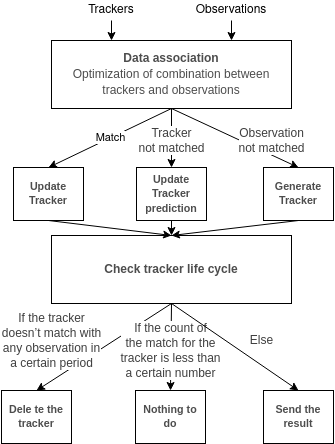
\includegraphics[width=0.5\linewidth]{figures/Autoware_Multi_Object_Tracking_Architecture.png}
    \caption{نحوه کارکرد گره ردیاب هم‌زمان چند جسم}
    \label{fig:Autoware_Multi_Object_Tracker}
\end{figure}

در گره ردیاب هم‌زمان چند جسم، از فیلتر‌های کالمن تعمیم‌یافته شده\LTRfootnote{\lr{EKF-Filter}} استفاده 
می‌شود تا وضعیت انواع اجسام مختلف حاضر در صحنه را تخمین بزند. این گره، مدل‌های ویژه‌ای را برای عابرین پیاده، دوچرخه‌‌ها، خوردو‌ها و وسایل نقلیه بزرگ تعریف کرده است، زیرا ابعاد آن‌ها بسیار متفاوت است و یک فیلتر کالمن جوابگوی تمام حالات نیست. این مدل‌ها به صورت موازی اجرا می‌شوند و بدین شکل، یک سیستم ردیاب پایدار و دقیق پیاده‌سازی می‌شود \cite{AWSIM:Documentation}.

\subsection{نتیجه‌گیری}
در این بخش، به این نتیجه رسیده شد که آموزش مدل‌های تشخیص اجسام سه‌بعدی، نیاز به مجموعه داده‌های عظیم دارد که خارج از توانایی این پژوهش است. راه‌حل پیشنهادی، استفاده از مدل‌های از پیش آموزش داده شده است. ایده‌ای که در این زمینه زده شد، استفاده از مدل هوش مصنوعی مورد استفاده ابزار \lr{Autoware}، برای تشخیص و ردیابی اجسام است. 

\section{اعمال مدل هوش‌ مصنوعی به ورودی لایدار}
در بخش قبلی، به این نتیجه رسیدیم که می‌توان از مدل‌ \lr{CenterPoint} مورد استفاده در ابزار \lr{Autoware}، به عنوان تشخیص دهنده اجسام استفاده کرد. همچنین می‌توان از گره ردیاب هم‌زمان چند جسم آن، برای ردیابی اجسام تشخیص داده شده استفاده کرد. با نگاهی دیگر به \cref{fig:Autoware_Perception_Detection_Node_Graph} که گراف گره مولفه ادراک است، درمی‌یابیم که گره‌ی \lr{lidar\_centerpoint}، دارای اشتراکی به یک مبحث\LTRfootnote{\lr{/sensing/lidar/concatenated/pointcloud}} است. این مبحث، خروجی پیش‌پردازش صورت گرفته بر روی ابر نقاط خام لایدار‌های خودروی خودران است. پس گمان می‌رود که با انتشار ابر نقاط خود به این مبحث، بتوانیم از لایه‌ی ادراک استفاده کنیم، که یعنی عملیات تشخیص و ردیابی بر روی ابر نقاط داده‌ی نمونه ما انجام شود.

جنس داده‌‌ی این مبحث، از نوع پیام‌های \lr{sensor\_msgs/PointCloud2} است. اما فرمت داده‌های ضبط شده‌ی لایدارهای شرکت \lr{Ouster}، فرمت \lr{*.pcap} است که در داخل آن بسته‌های\LTRfootnote{\lr{Packet}} شبکه‌ای لایدار ذخیره شده‌اند. پس نیاز است که این بسته‌ها در درجه اول پردازش شوند، و سپس اطلاعات ابر نقاط داخل هر بسته آن به پیامی از جنس \lr{PointCloud2}، که از پیام‌های پیش‌فرض برای ابر نقاط در بستر \lr{ROS2} است، تبدیل بشوند. به همین منظور، کدی در بستر \lr{ROS2} نوشته شد، که داده‌های بلادرنگ یا ضبط‌ شده‌ی لایدار‌های \lr{Ouster} را به ابر نقاط مورد استفاده در \lr{ROS2}، تبدیل کند. 
این بسته \lr{ROS2} که \lr{"pcap\_to\_pointcloud2\_publisher\_py"} نام دارد، با استفاده از کتابخانه کلاینت \lr{rclpy} نوشته شده است که با استفاده از آن می‌توان از کتابخانه‌های ‌\lr{ROS2} در زبان برنامه‌نویسی پایتون\LTRfootnote{\lr{Python Programming Language}} استفاده کرد. در این بسته، با استفاده از کتابخانه \lr{OusterSDK}، داده‌های \lr{.pcap} خوانده می‌شوند و سپس با استفاده از کانال فاصله لایدار، مختصات کارتزین ابر نقاط هر فریم بدست می‌آید. همچنین شدت سیگنال بازتابی هر کدام از نقاط با استفاده از کانال انعکاس‌پذیری به دست می‌آید. سپس با استفاده از کتابخانه رابط \lr{PointCloud2} که برای بسته \lr{ROS2} است، این نقاط را به همراه سرایند\LTRfootnote{\lr{Header}} که در آن زمان انتشار پیام به همراه دستگاه مختصاتی مربوط به آن است، منتشر می‌کند.

\begin{figure}[h!]
    \centering
    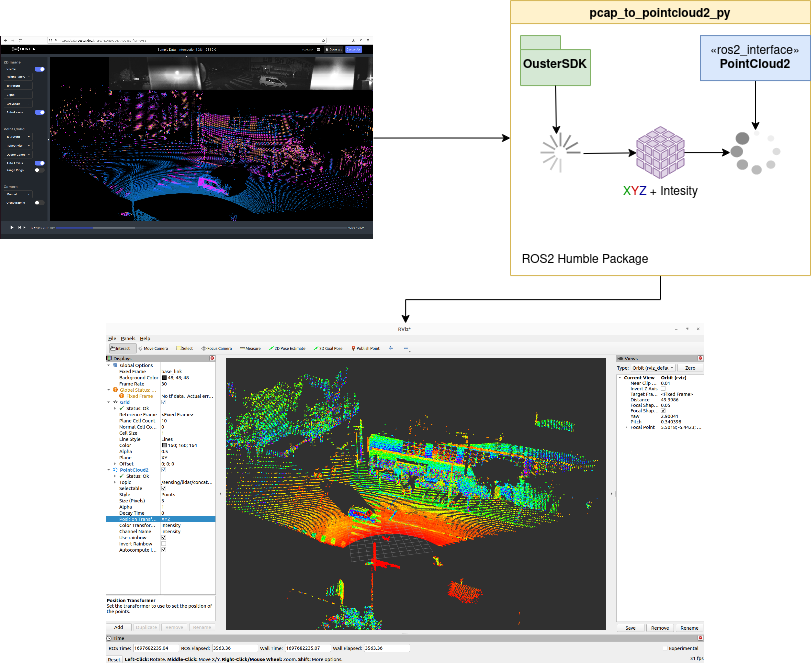
\includegraphics[width=1\linewidth]{figures/pcap_to_pointcloud2.png}
    \caption{روند تبدیل داده‌های ضبط شده لایدار به پیام \lr{PointCloud2} و انتشار آن.}
    \label{fig:pcap_to_pointcloud2}
\end{figure}

در \cref{fig:pcap_to_pointcloud2}، شماتیکی از روند تبدیل داده‌ی \lr{.pcap} ضبط شده توسط \lr{Ouster Studio}، به عنوان ورودی به بسته \lr{pcap\_to\_pointcloud2} داده شده است و نتیجه آن در محیط \lr{RViz2}، که محیطی برای مشاهده مبحث‌های \lr{ROS2} است، مشاهده می‌شود.

\subsection{دستکاری فایل‌های اجرایی \lr{Autoware}}
پس با موفقیت توانستیم این تبدیل داده را پیاده‌سازی کنیم. این ابر نقاط تبدیل شده، با فرکانس ۱۰ هرتز بر روی مبحث مورد استفاده توسط مولفه ادراک، انتشار می‌یابد. حال برای اینکه مولفه ادراک به درستی بتواند عملیات تشخیص را بر روی ابر نقاط ورودی انجام دهد، نیاز است تا فایل‌های اجرایی‌اش\LTRfootnote{\lr{Launch Files}} دستکاری شوند و برخی از فیلتر‌های آن غیرفعال شوند. پس لازم است تا معماری فایل‌های اجرایی \lr{Autoware} را درک کنیم و آنها را دستکاری کنیم. فایل‌های اجرایی این ابزار از چند لایه تشکیل شده‌اند که آنها را گام به گام شرح می‌دهیم. در ابتدا نگاهی به معماری فایل اجرایی اصلی \lr{Autoware} می‌اندازیم. در این فایل اجرایی، همه‌ی مولفه‌های اصلی و مهم \lr{Autoware} بصورت موازی اجرا می‌شوند. \cref{fig:Autoware_Launch} نشان‌دهنده معماری این فایل اجرایی است. هر کدام از مولفه‌ها با مثبت بودن متغیر متناظرشان، می‌توانند اجرا شوند. یعنی کاربر این قابلیت اجرا نکردن مولفه‌هایی که نیاز ندارد را دارد.

\begin{figure}[h!]
    \centering
    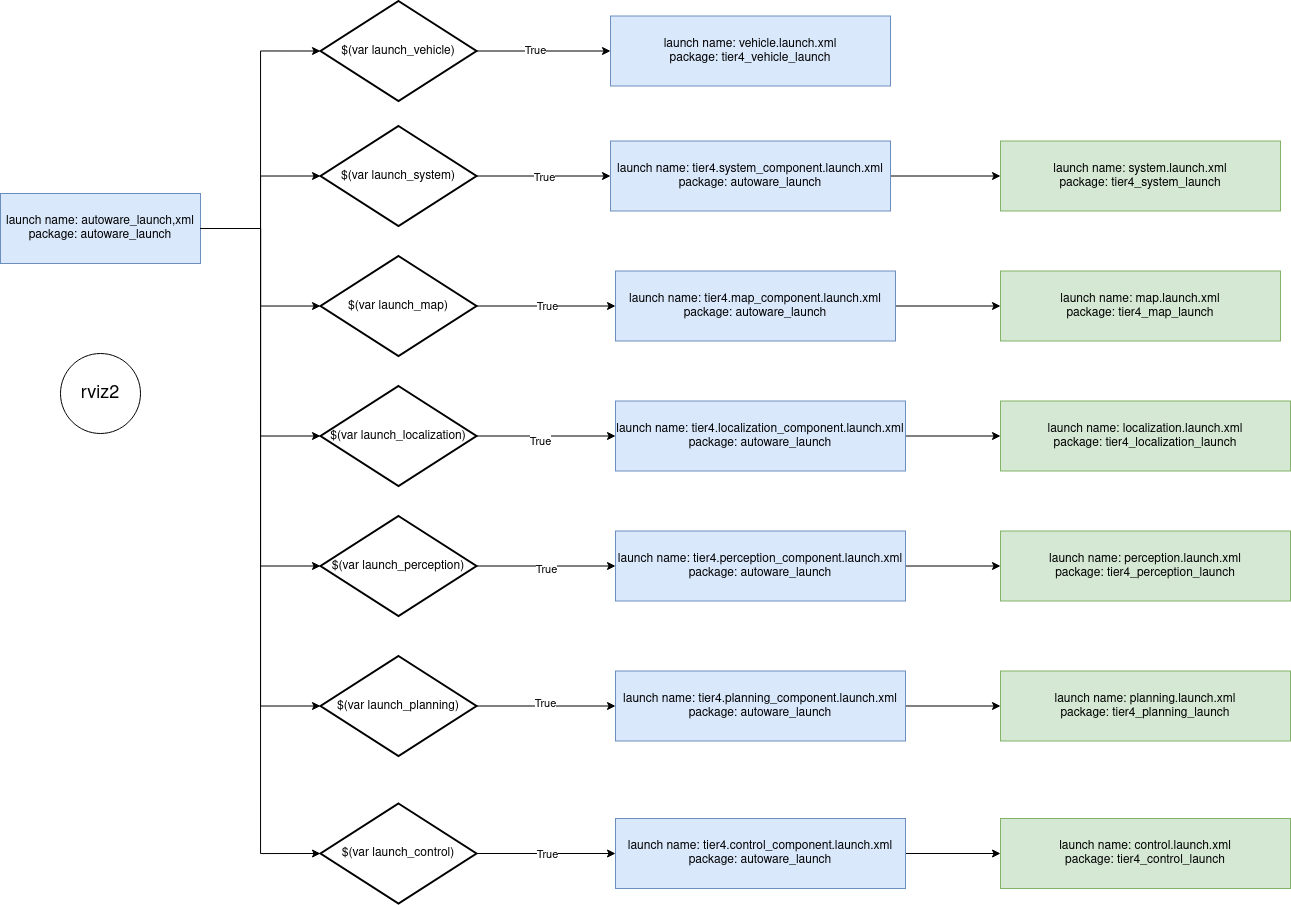
\includegraphics[width=0.75\linewidth]{figures/autoware_launch.png}
    \caption{معماری فایل اجرایی اصلی \lr{autoware\_launch}}
    \label{fig:Autoware_Launch}
\end{figure}

از آنجایی که ما فقط به مولفه ادراک \lr{Autoware} نیاز داریم، متغیرهای متناظر مولفه‌های دیگر را همانند \cref{fig:Autoware_Launch_Settings} منفی می‌گذاریم.

\begin{figure}[h!]
    \centering
    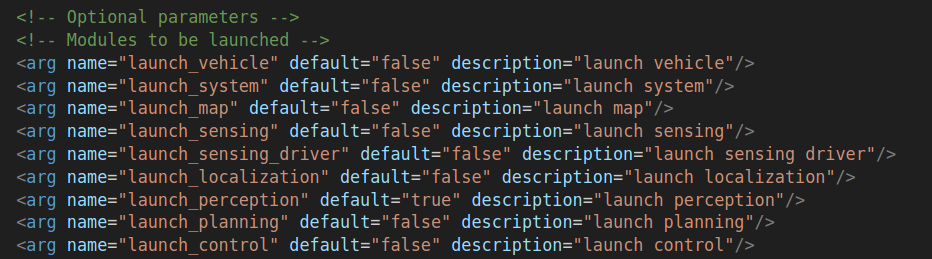
\includegraphics[width=0.75\linewidth]{figures/autoware_launch_settings.png}
    \caption{منفی گذاشتن تمامی مولفه‌ها بجز مولفه ادراک}
    \label{fig:Autoware_Launch_Settings}
\end{figure}

گام بعدی، نگاه انداختن به فایل اجرایی مولفه ادراک است. در \cref{fig:Autoware_Perception_Launch} مشاهده می‌کنیم که این مولفه، از سه فایل اجرایی اصلی به نام‌های \lr{detection.launch}، \lr{tracking.launch} و \lr{prediction.launch} استفاده می‌کند. کار اصلی ما با دو فایل اجرایی اول است. فایل اجرایی سوم  به نقشه‌ی برداری از محل مورد نظر نیاز دارد، که در حال حاضر آن را نداریم، پس آن را غیرفعال می‌کنیم. دو فایل اجرایی دیگر نیز در فایل اجرایی مولفه ادراک هستند که در شکل کشیده نشده‌اند. این فایل‌های اجرایی مربوط به گره‌های پیش‌پردازشی بخش‌بندی اجسام و نقشه شبکه اشغال احتمالاتی هستند. از آنجایی که این لایه‌های پیش‌پردازش مفید هستند، آن‌ها را دستکاری نمی‌کنیم.

\begin{figure}[h!]
    \centering
    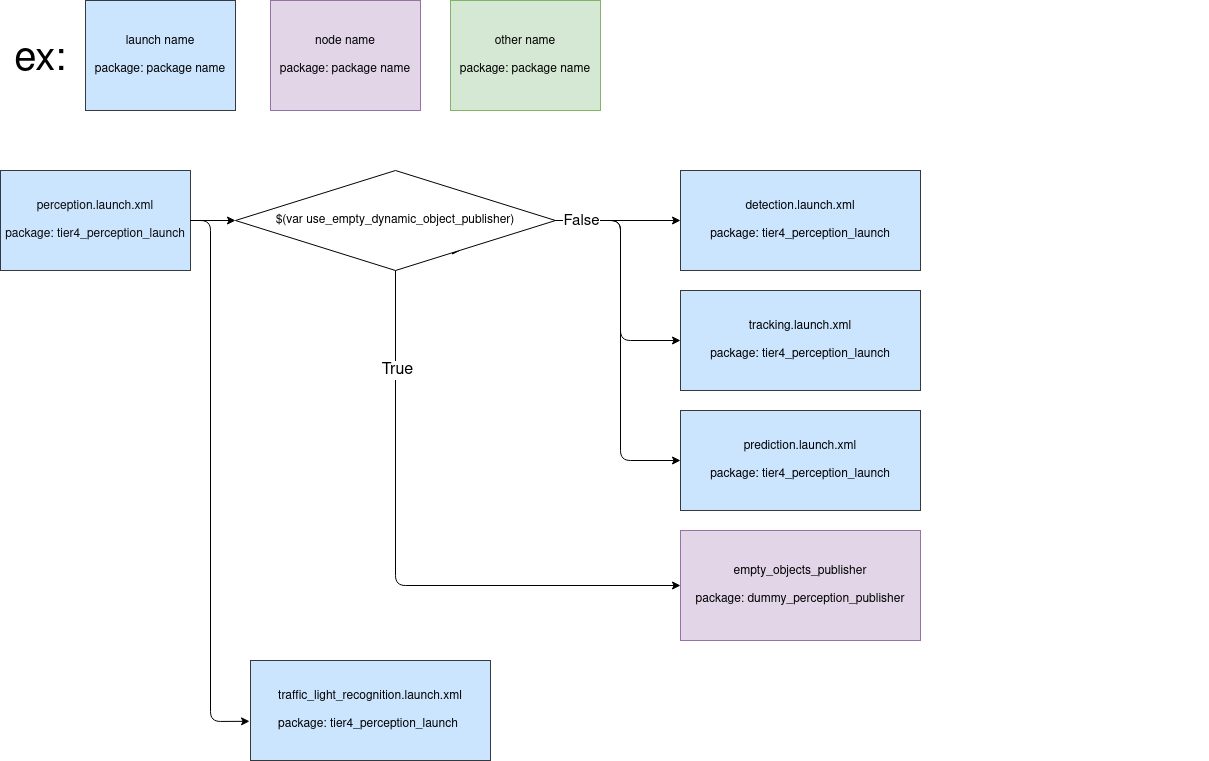
\includegraphics[width=0.75\linewidth]{figures/Autoware_Perception_Launch.png}
    \caption{معماری فایل‌های اجرایی \lr{perception.launch}\cite{Autoware_Universe:Documentation}}
    \label{fig:Autoware_Perception_Launch}
\end{figure}

گام بعدی، نگاه کردن به معماری فایل اجرایی \lr{detection.launch} است. در این فایل اجرایی، انواع فایل‌های اجرایی برای تشخیص‌دهنده‌های مختلف نوشته شده‌اند. همچنین مُد پیش‌فرض بر روی حالت \lr{lidar} گذاشته شده است و نیازی به اعمال تغییر نیست. \cref{fig:detection_launch}، معماری این فایل اجرایی را نشان می‌دهد.

\begin{figure}[h!]
    \centering
    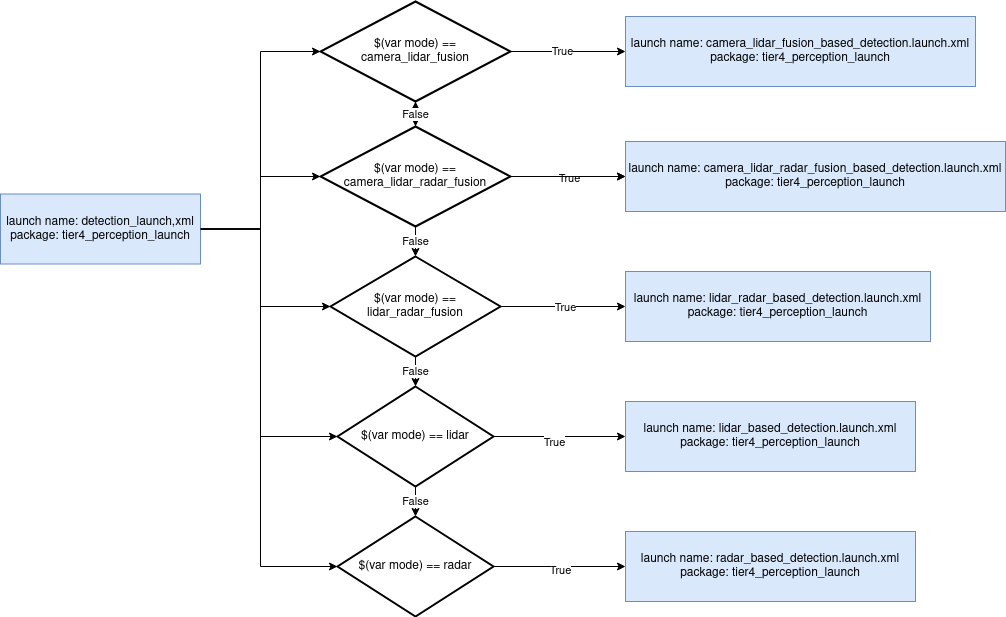
\includegraphics[width=0.75\linewidth]{figures/detection_launch.png}
    \caption{معماری فایل‌ اجرایی \lr{detection.launch}}
    \label{fig:detection_launch}
\end{figure}

حال نگاهی به فایل اجرایی \lr{lidar\_based\_detection.launch} می‌اندازیم. این فایل برای اجرای تشخیص‌دهنده‌ی مبتنی بر ابر نقاط است. \cref{fig:lidar_based_detection}، معماری این فایل اجرایی را نشان می‌دهد. در این فایل اجرایی، به صورت پیش‌فرض، از مدل تشخیص سه‌بعدی \lr{CenterPoint} استفاده می‌شود. همچنین به صورت پیش‌فرض، برخی از گره‌های فیلتر همانند گره فیلتر لینلت، فیلتر اعتبارسنجی موانع براساس ابر نقاط و فیلتر براساس نقشه ابر نقاط نیز اجرا می‌شوند. گره‌های دیگر همانند خوشه‌بندی اقلیدسی، تخمین شکل جسم، ادغام‌کننده اجسام و تشخیص براساس ردیاب نیز مشاهده می‌شوند. از بین همه این گره‌ها، دو گره‌ی فیلتر لینلت و فیلتر براساس نقشه ابرنقاط بایستی خاموش شوند، زیرا نقشه بُرداری و نقشه ابرنقاط نداریم. 

\begin{figure}[h!]
    \centering
    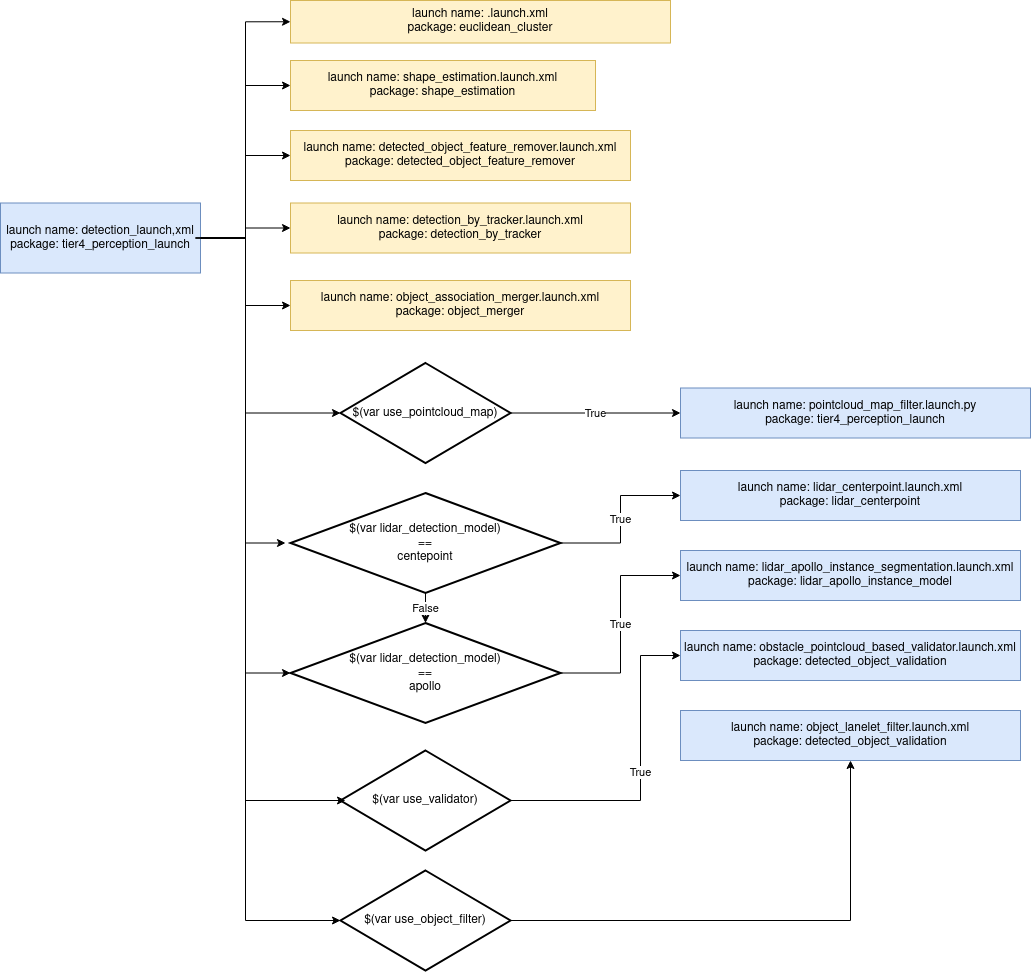
\includegraphics[width=0.7\linewidth]{figures/lidar_based_detection.png}
    \caption{معماری فایل‌ اجرایی \lr{lidar\_based\_detection.launch}}
    \label{fig:lidar_based_detection}
\end{figure}

\subsection{نتیجه‌گیری}

در بخش قبلی معماری فایل‌های اجرایی مولفه ادراک \lr{Autoware} را مشاهده کردیم. تغییراتی که بایستی اعمال شوند عبارتند از:
\begin{enumerate}
    \item خاموش کردن بقیه مولفه‌ها بجز مولفه ادراک، در فایل \lr{autoware\_launch}
    \item خاموش کردن فایل اجرایی \lr{prediction.launch}، در فایل اجرایی \lr{perception.launch}
    \item خاموش کردن فایل‌های اجرایی مربوط به گره‌های فیلتر لینلت و فیلتر موانع براساس نقشه ابر نقاط، در فایل اجرایی \lr{lidar\_based\_detection.launch}
\end{enumerate}
برای اینکه خود فایل‌های اجرایی \lr{Autoware} خراب نشوند، فایل‌های اجرایی جدای سفارشی‌سازی شده نسبت به نیازمندی‌هایمان نوشته شده است، که با پیشوند \lr{digital\_twin\_*} شروع می‌شوند. این فایل‌ها در ساختار پوشه‌ای فایل‌های اجرایی \lr{Autoware} جایگذاری شده‌اند.
حال وقت تست کردن تشخیص دهنده سه‌بعدی رسیده است. \cref{fig:3D_Detection_Run_Commands} دستور‌های لازم برای اجرای تشخیص‌دهنده سفارشی‌سازی شده نسبت به نیازهایمان را نشان می‌دهد. 
\begin{figure}[h!]
    \centering
    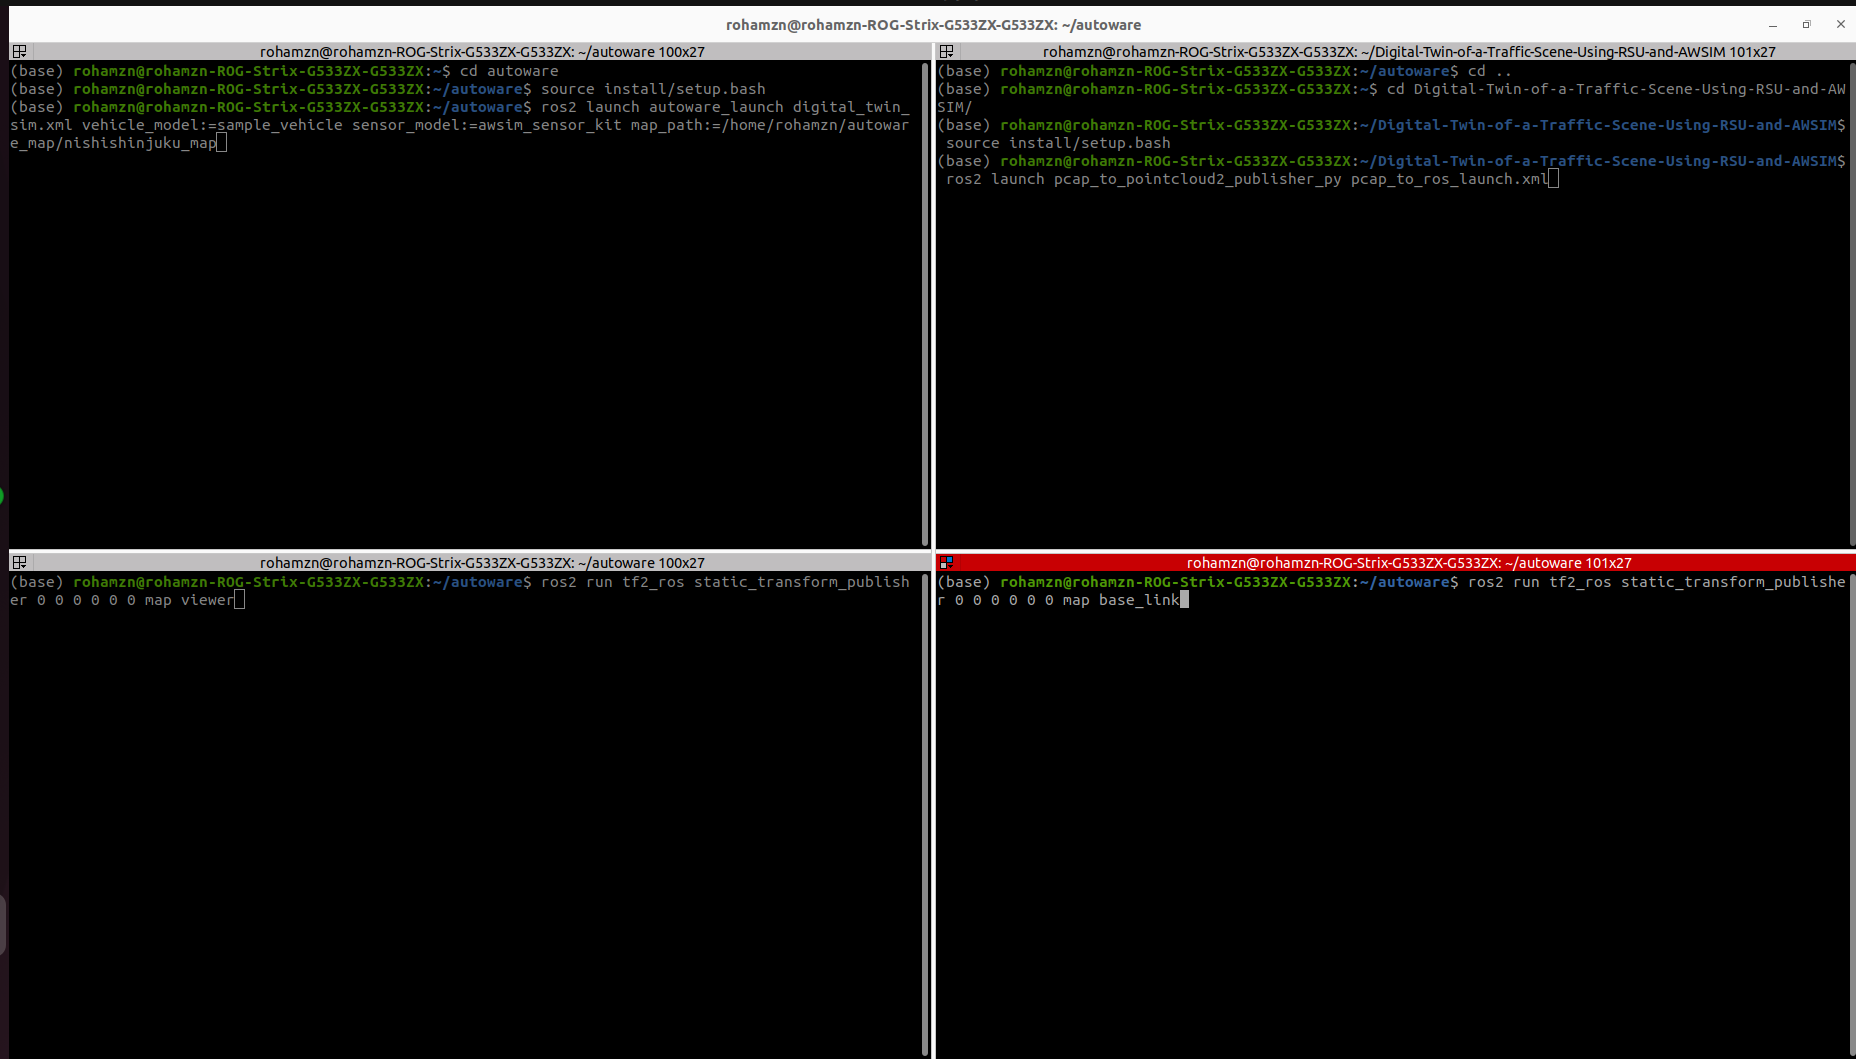
\includegraphics[width=1\linewidth]{figures/3D_Detection_Run_Commands.png}
    \caption{دستور‌های اجرایی تشخیص‌دهنده سه‌بعدی}
    \label{fig:3D_Detection_Run_Commands}
\end{figure}
لازم به ذکر است که در دو ترمینال پایین، ماتریس‌های تبدیل و دوران لایدار نسبت به سطح زمین و همچنین زمین نسبت به تماشاگر نیز بایستی به صورت دستی وارد شوند. دلیل اینکار به هم‌راستا نبودن لایدار‌های نصب شده بر روی خودروی خودران، نسبت به محور‌های مختصاتی ‌\lr{ROS2} است. در ادامه به توضیح بیشتر این مشکل، می‌پردازیم.
حال طبق \cref{fig:3D_Detection_Run_Commands} دستورات را اجرا می‌کنیم و نتیجه زیر را مشاهده می‌کنیم:
\begin{figure}[h!]
    \centering
    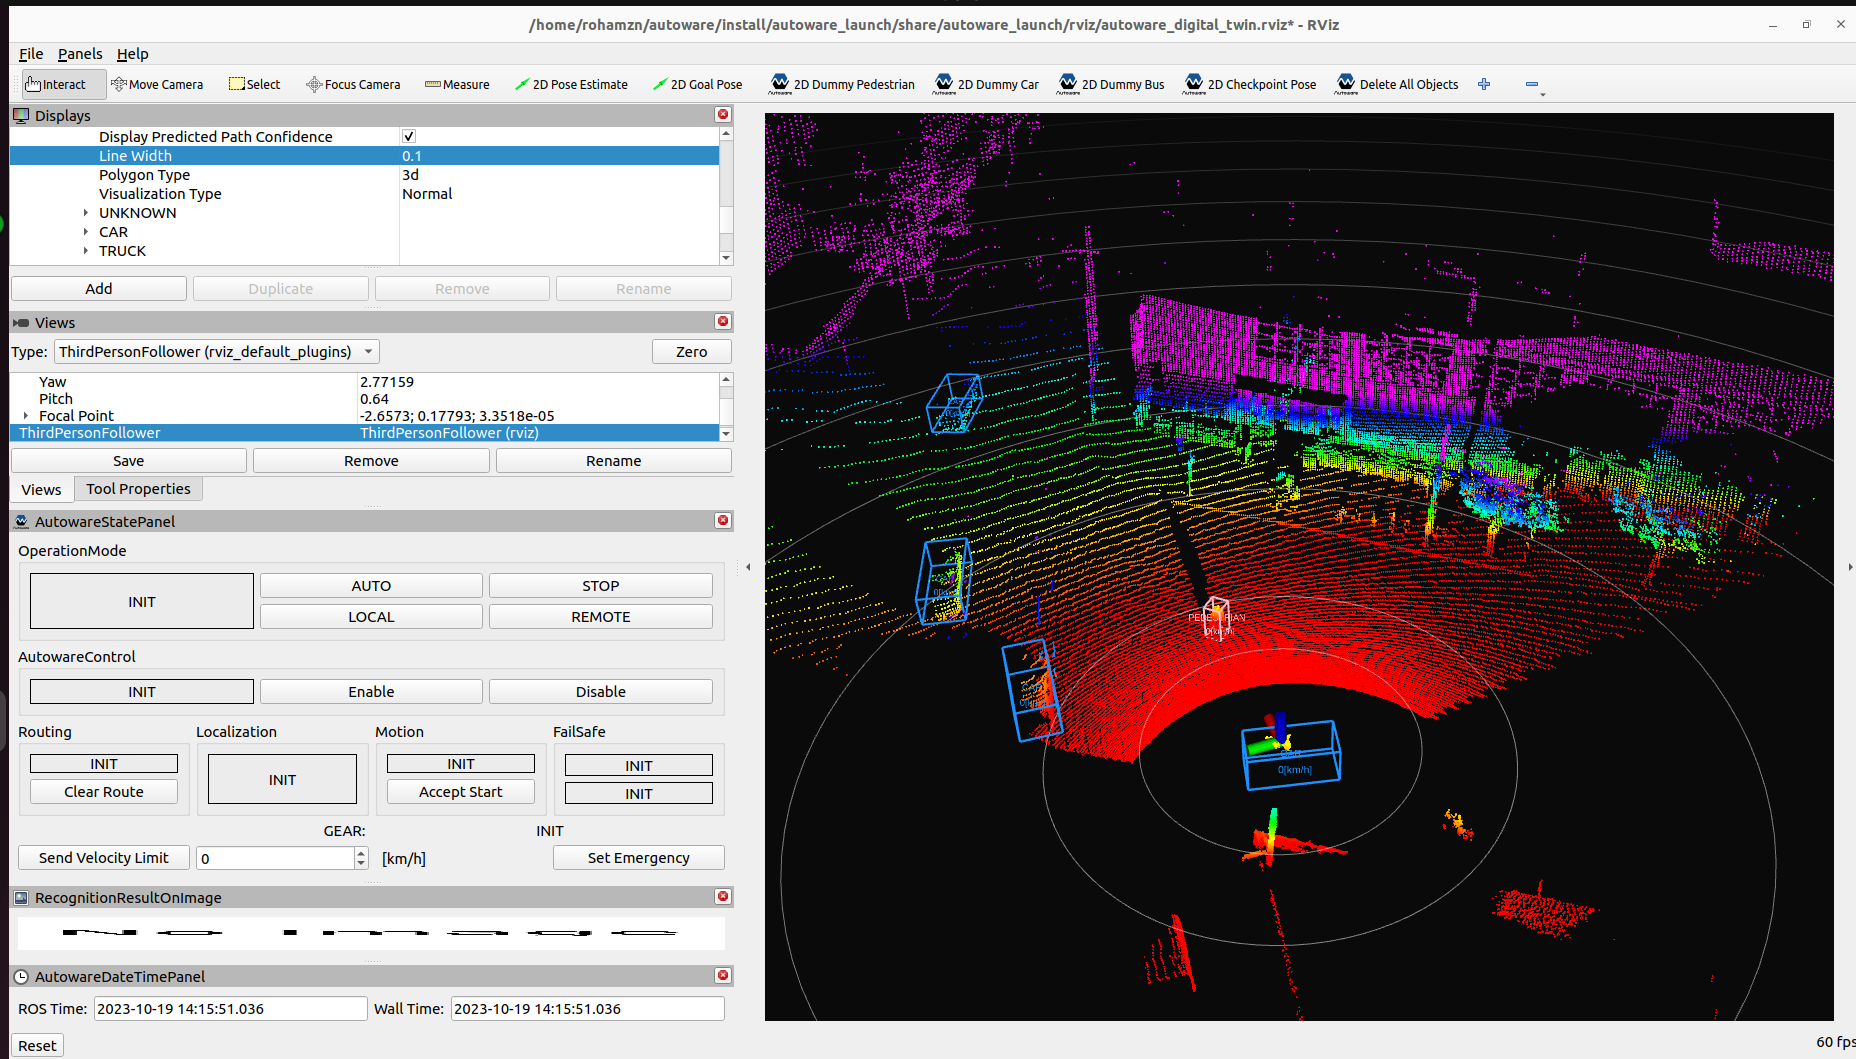
\includegraphics[width=0.85\linewidth]{figures/3D_Object_Detection.png}
    \caption{اجرایی از تشخیص اجسام سه‌بعدی توسط مدل \lr{CenterPoint}  در داده‌ی نمونه یک چهارراه}
    \label{fig:3D_Object_Detection}
\end{figure}

تشخیص دهنده ‌استفاده شده، قابلیت تشخیص عابرین پیاده، دوچرخه سوار، موتور، خودرو، اتوبوس و کامیون را دارد.
\cref{fig:3D_Detection_Driving} نیز نشان می‌دهد که تنها با انتشار داده‌ نمونه دیگری که از شرکت \lr{Ouster} گرفته شده است (یا هر ضبط لایدار با فرمت \lr{.pcap})، می‌توان عملیات تشخیص بلادرنگ را بر روی آن اعمال کرد.

\begin{figure}[h!]
    \centering
    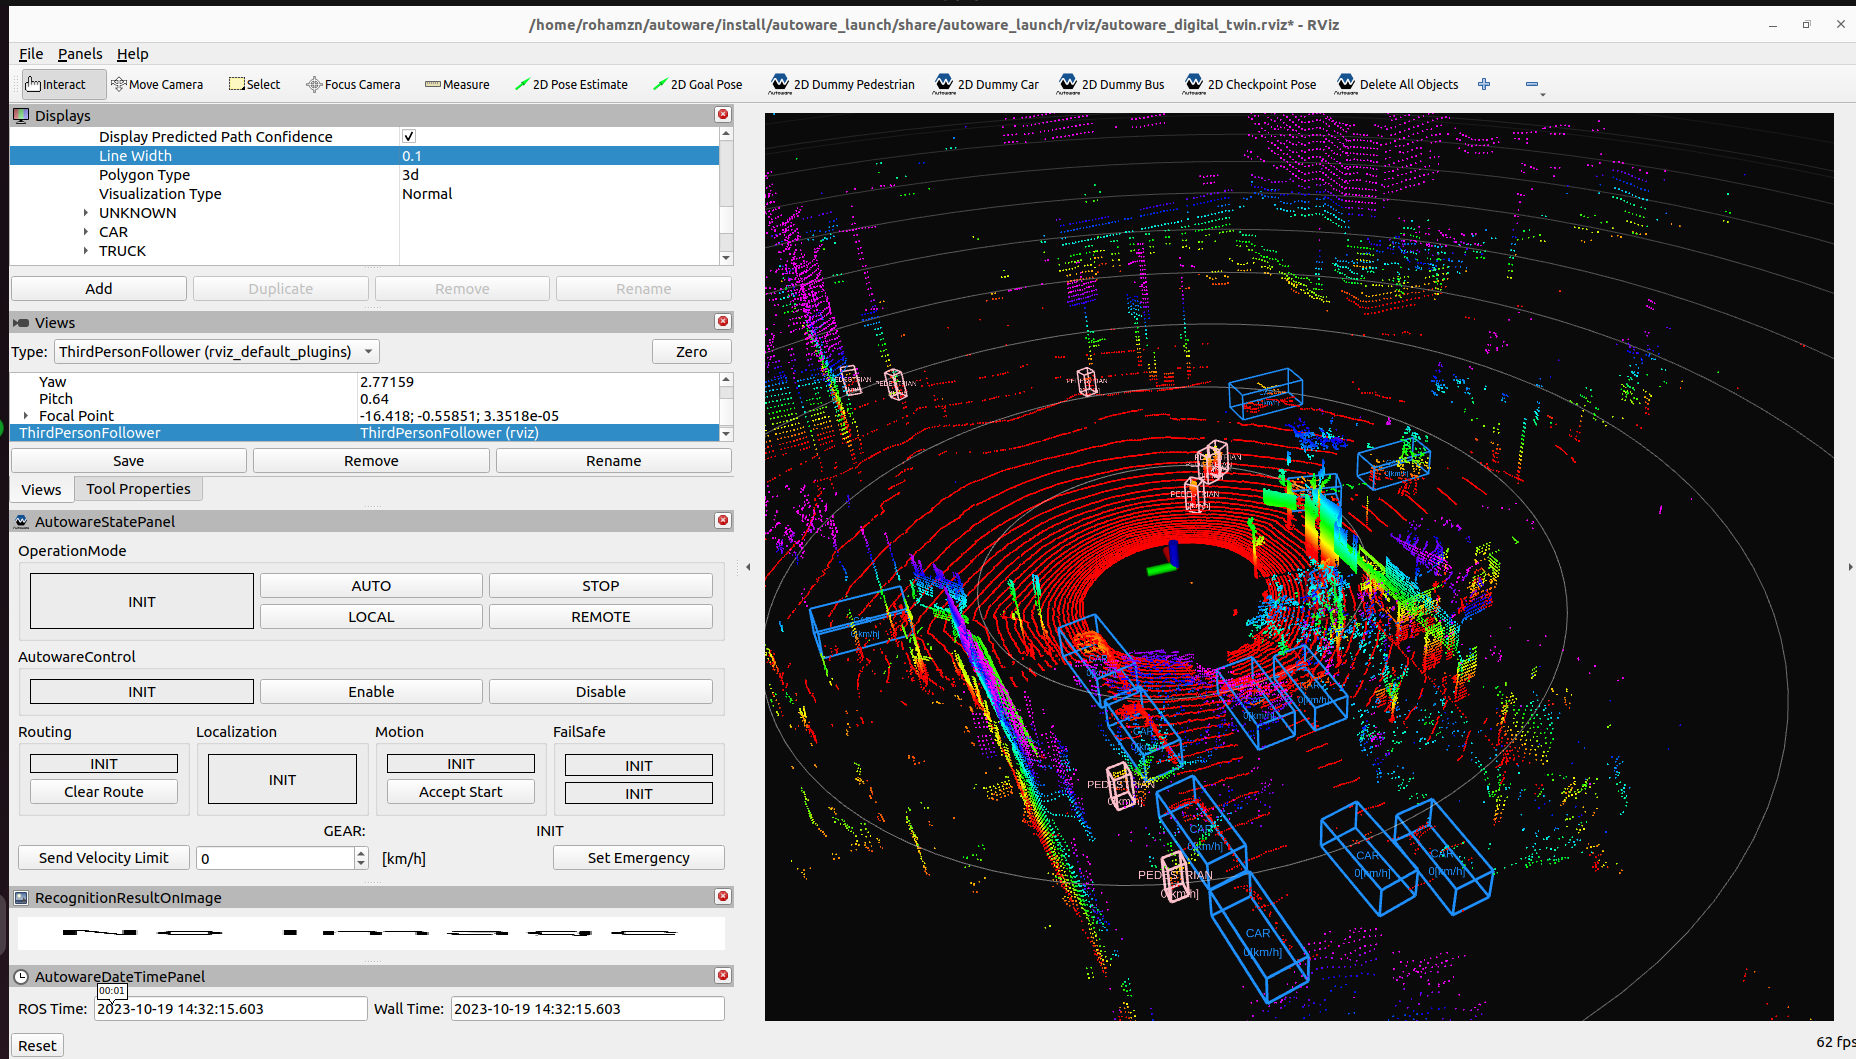
\includegraphics[width=0.9\linewidth]{figures/3D_Detection_Driving.png}
    \caption{اجرایی از تشخیص اجسام سه‌بعدی توسط مدل \lr{CenterPoint} در داده‌ی نمونه یک ماشین در حال رانندگی در سطح شهر}
    \label{fig:3D_Detection_Driving}
\end{figure}

\begin{figure}[h!]
    \centering
    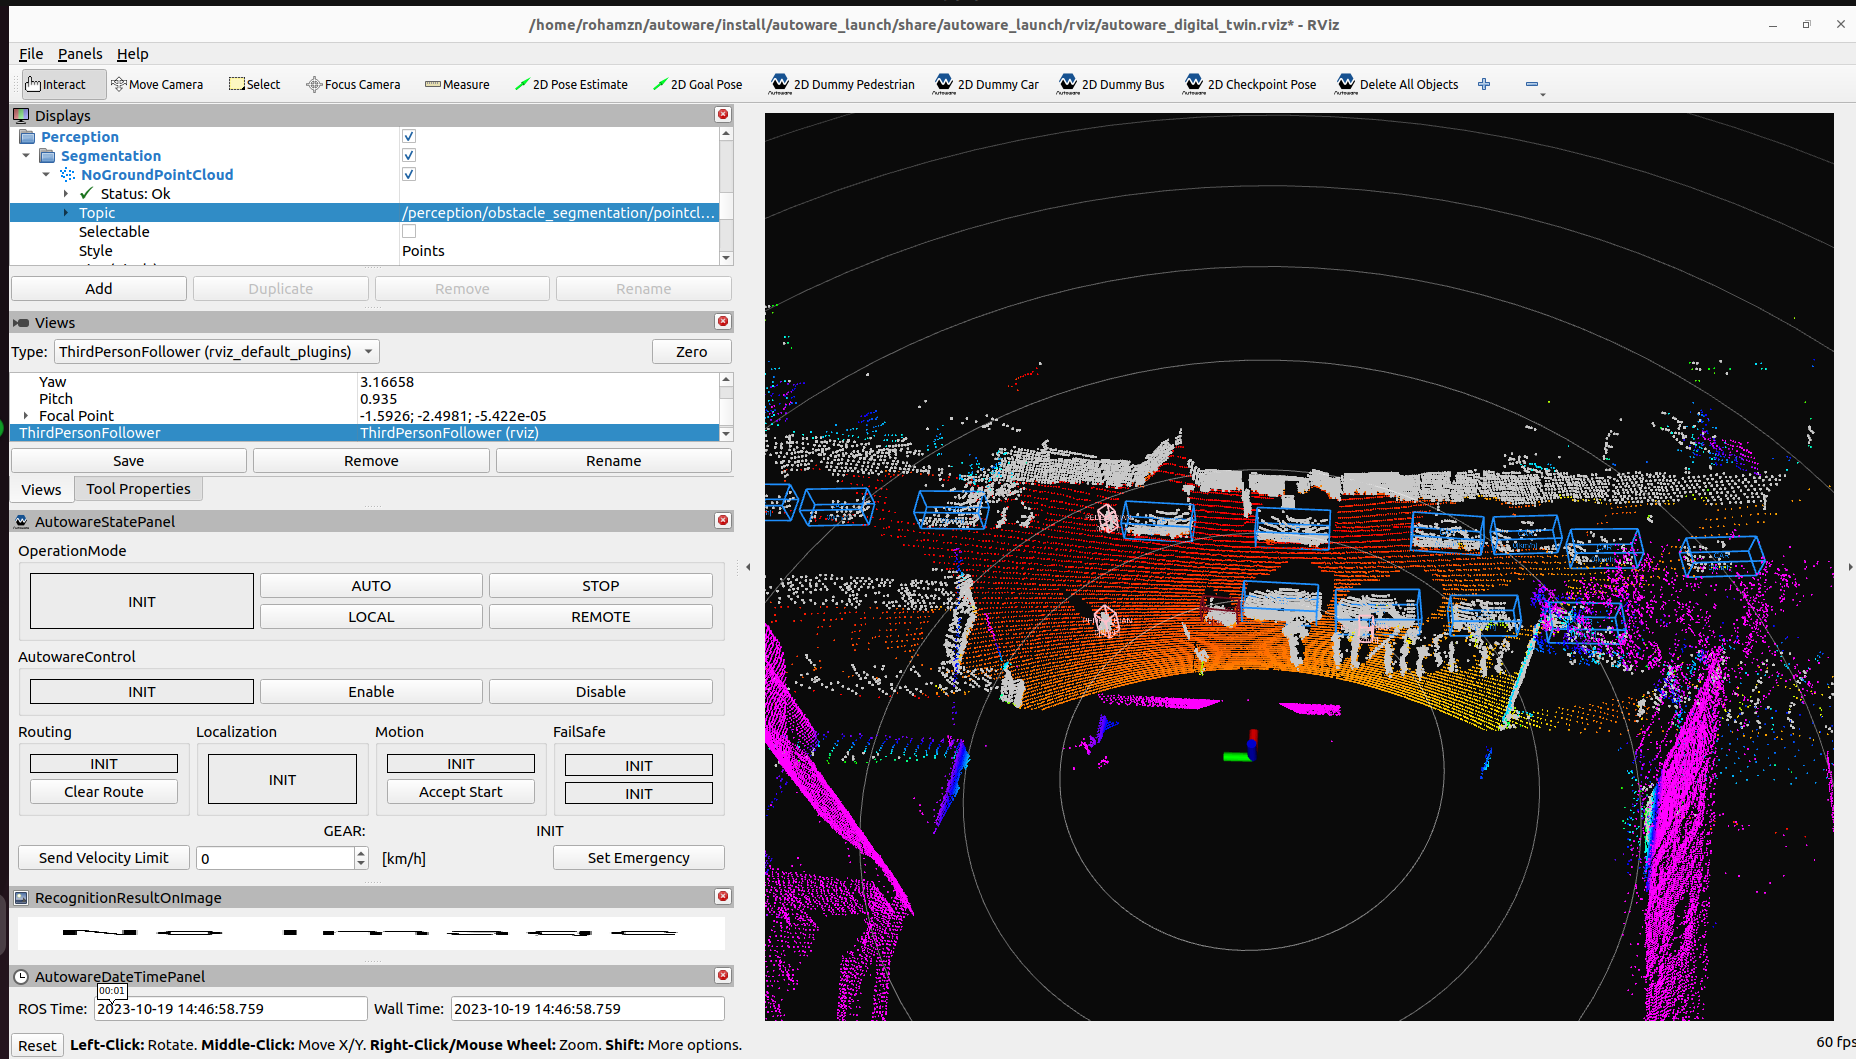
\includegraphics[width=0.9\linewidth]{figures/3D_Obstacle_Segmentation.png}
    \caption{مشاهده خروجی بخش‌بندی موانع، که نقاط زمین و نویزها را از ابر نقاط فیلتر می‌کند.}
    \label{fig:3D_Obstacle_Segmentation}
\end{figure}

با توجه به \cref{fig:Autoware_Perception_Detection_Node_Graph}، می‌توان مشاهده کرد که هر کدام از گره‌ها بر روی چه مبحثی، خروجی‌های خود را انتشار می‌کنند. در محیط \lr{RViz2} می‌توان در این مباحث اشتراک گرفت و خروجی‌های آن را مشاهده کرد. به طور مثال در شکل‌های فوق، اشتراک در مبحثی\LTRfootnote{\lr{/perception/object\_recognition/detection/centerpoint/validation/objects}} گرفته شده است که در آن مختصات، ابعاد کادر محصورکننده و برچسب اجسام فیلتر شده براساس گره اعتبارسنجی اجسام بر اساس ابر نقاط، منتشر می‌شوند. به طور مثال می‌توانیم در مبحث بخش‌بندی موانع\LTRfootnote{\lr{/perception/obstacle\_segmentation/pointcloud}}، که خروجی گره پیش‌پردازش مولفه ادراک است، اشتراکی بگیریم. \cref{fig:3D_Obstacle_Segmentation} نتیجه‌ی گرفتن اشتراک در این مبحث، با استفاده از نمایشگر \lr{RViz2} است.

\section{پردازش ویژگی‌های اجسام تشخیص داده شده در شبیه‌ساز}
در بخش قبلی با موفقیت توانستیم مدلی را پیدا کنیم و با استفاده از آن، تشخیص بلادرنگ اجسام سه‌بعدی را در داده‌های نمونه لایدار \lr{Ouster} انجام دهیم. طبق \cref{fig:Autoware_Perception_Detection_Node_Graph}، می‌توان مشاهده کرد که ورودی گره‌ی ردیاب ‌هم‌زمان چند جسم یا همان \lr{multi\_object\_tracker}، خروجی گره‌ی ادغام کننده اجسام است. همچنین با مشاهده فایل‌های اجرایی و کد این ردیاب، نتیجه گرفته شد که خروجی این گره، بر روی مبحثی\LTRfootnote{\lr{/perception/object\_recognition/tracking/objects}} منتشر می‌شود.

\begin{figure}[h!]
    \centering
    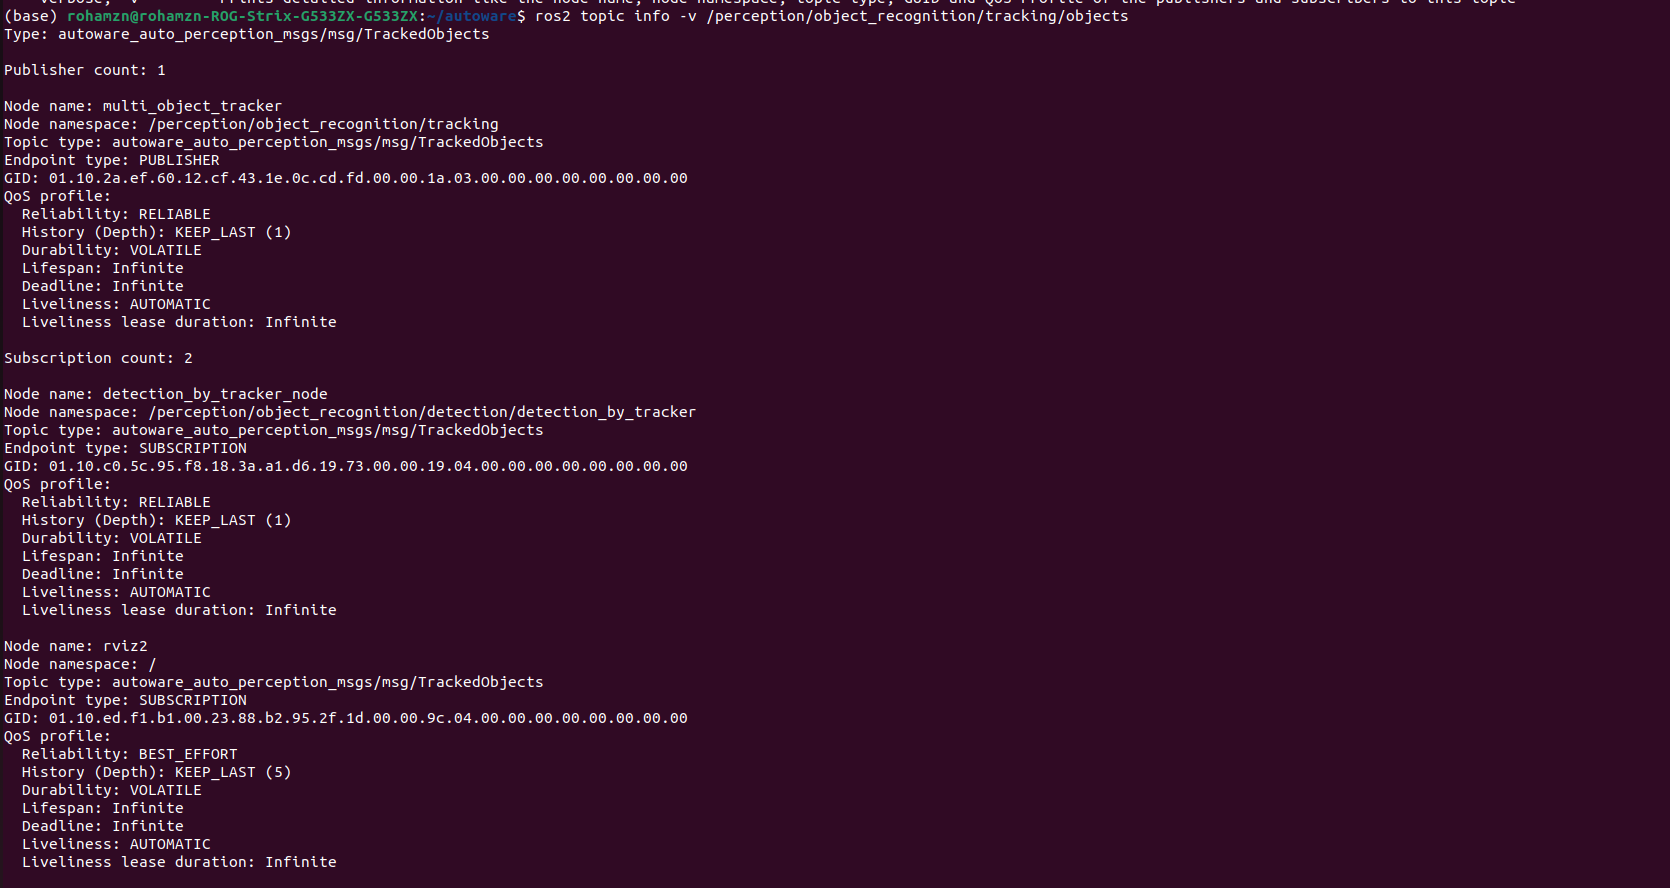
\includegraphics[width=1\linewidth]{figures/Tracked_Objects_Topic_Info.png}
    \caption{مشخصات مبحث خروجی گره‌ ردیاب هم‌زمان چند جسم}
    \label{fig:Tracked_Objects_Topic_Info}
\end{figure}

خروجی این مبحث برای این پژوهش بسیار ارزشمند است، زیرا تمام ویژگی‌های اجسام تشخیص داده شده اعم از سرعت، شتاب، جهت، شناسه یکتا و برچسب در آن موجود است. \cref{fig:Tracked_Objects_Topic_Info} مشخصات این مبحث را نشان می‌دهد. مشاهده می‌شود که جنس پیام‌های انتشار یافته در این مبحث، از نوع \lr{autoware\_auto\_perception\_msgs/msg/TrackedObjects} است.

\begin{figure}
    \centering
    \begin{latin}
        \begin{lstlisting}[style=code]
#include "autoware_auto_perception_msgs/msg/TrackedObject.idl"
#include "std_msgs/msg/Header.idl"
        
module autoware_auto_perception_msgs {
module msg {
    @verbatim (language="comment", text=
    " This is the output of object tracking and the input to prediction.")
    struct TrackedObjects {
    std_msgs::msg::Header header;
    sequence<autoware_auto_perception_msgs::msg::TrackedObject> objects;
    };
};
        \end{lstlisting}
    \end{latin}
    \caption{کد مربوط به ساختار پیام خروجی ردیاب هم‌زمان چند جسم}
    \label{fig:Tracked_Objects_Code}
\end{figure}

\begin{figure}[h!]
    \centering
    \begin{latin}
        \begin{lstlisting}[style=code]
#include "autoware_auto_perception_msgs/msg/ObjectClassification.idl"
#include "autoware_auto_perception_msgs/msg/Shape.idl"
#include "autoware_auto_perception_msgs/msg/TrackedObjectKinematics.idl"
#include "unique_identifier_msgs/msg/UUID.idl"

module autoware_auto_perception_msgs {
  module msg {
    struct TrackedObject {
      unique_identifier_msgs::msg::UUID object_id;

      @range (min=0.0, max=1.0)
      float existence_probability;

      sequence<autoware_auto_perception_msgs::msg::ObjectClassification> classification;
      autoware_auto_perception_msgs::msg::TrackedObjectKinematics kinematics;

      autoware_auto_perception_msgs::msg::Shape shape;
    };
  };
};
        \end{lstlisting}
    \end{latin}
    \caption{کد مربوط به ساختار پیام جسم در حال ردیابی}
    \label{fig:Tracked_Object_Code}
\end{figure}

\cref{fig:Tracked_Objects_Code}، نشان ‌می‌دهد که این پیام در داخل خود آرایه‌ای از اجسام در حال ردیابی دارد که از جنس \lr{autoware\_auto\_perception\_msgs/msg/TrackedObject} هستند. \cref{fig:Tracked_Object_Code} نیز، ساختار پیام‌ هر جسم در حال ردیابی را نشان می‌دهد. همانطور که مشاهده می‌کنیم، به هر جسم شناسه‌ای یکتا\LTRfootnote{\lr{Universally Unique Identifier: UUID}} داده می‌شود. همچنین درصد احتمال وجود\LTRfootnote{\lr{Existence Probability}} آنها با استفاده از روش‌های مختلف محاسبه شده است. 
در آخر نیز سه داده‌ی مهم داریم که به ترتیب طبقه‌بندی\LTRfootnote{\lr{Classification}}، سینماتیک\LTRfootnote{\lr{Kinematics}} و شکل جسم\LTRfootnote{\lr{Shape}} را در خود جای می‌دهند. 

جفت پیام‌های بررسی شده، زیرمجموعه بسته پیام‌های \lr{autoware\_auto\_perception\_msgs}\LTRfootnote{\lr{autoware\_auto\_perception\_msgs Package}} می‌باشند و با بهره‌بری از این بسته، می‌توان پیام‌های فوق را خواند و پردازش کرد. بخاطر داریم که در شبیه‌ساز \lr{AWSIM}، از افزونه \lr{R2FU} استفاده می‌شود و با استفاده از آن می‌توان در مباحث \lr{ROS2} اشتراک گرفت و یا به آنها داده منتشر کرد. در \cref{tab:R2FU_Messages_Table}، تمامی پیام‌هایی که توسط این افزونه به صورت پیش‌فرض پشتیبانی شده‌اند نوشته شده است. مشاهده می‌کنیم که پیام‌های بسته \lr{autoware\_auto\_perception\_msgs} توسط این افزونه پشتیبانی نمی‌شوند و در نتیجه نمی‌توان پیام‌های گره‌ی ردیاب هم‌زمان چند جسم را به خواند و پردازش کرد. \begin{figure}[h!]
    \centering
    \begin{latin}
        \begin{lstlisting}[style=codecs]
[SerializeField] string detectedObjectsTopic = "/perception/object_recognition/tracking/objects";
[SerializeField] string detectedObjectsPublisherTopic = "/unity/perception/object_recognition/tracking/objects";

ISubscription<autoware_auto_perception_msgs.msg.TrackedObjects> trackedObjectsSubscriber;
IPublisher<autoware_auto_perception_msgs.msg.TrackedObjects> trackedObjectsPublisher;

trackedObjectsPublisher = SimulatorROS2Node.CreatePublisher<autoware_auto_perception_msgs.msg.TrackedObjects>(detectedObjectsPublisherTopic, qos);
trackedObjectsSubscriber = SimulatorROS2Node.CreateSubscription<autoware_auto_perception_msgs.msg.TrackedObjects>(detectedObjectsTopic, 
        msg => {trackedObjectsPublisher.Publish(msg);}, qos);
        \end{lstlisting}
    \end{latin}
    \caption{کد مربوط گرفتن اشتراک برای مبحث ردیاب و انتشار به یک مبحث جدید}
    \label{fig:Unity_Subscription_Code}
\end{figure}
ابزار \lr{AWSIM} در مستندات خود، روشی را برای اضافه کردن بسته‌های پیام دلخواه به افزونه \lr{R2FU}، مطرح کرده‌ است\LTRfootnote{\url{https://tier4.github.io/AWSIM/Components/ROS2/AddACustomROS2Message/}}. با پیش‌روی طبق دستورات مستندات \lr{AWSIM}، پیام‌های بسته ادراک نیز به این افزونه اضافه شدند. حال موتور \lr{Unity} می‌تواند با استفاده از کد \cref{fig:Unity_Subscription_Code}، در مباحث مورد نظر اشتراک بگیرد.
طبق کد، اگر بتوانیم به درستی پیام‌های ردیابی را در بستر \lr{Unity} بخوانیم، بایستی بتوانیم آن‌ها را به مبحثی جدید نیز منتشر کنیم.
\begin{figure}[h!]
    \centering
    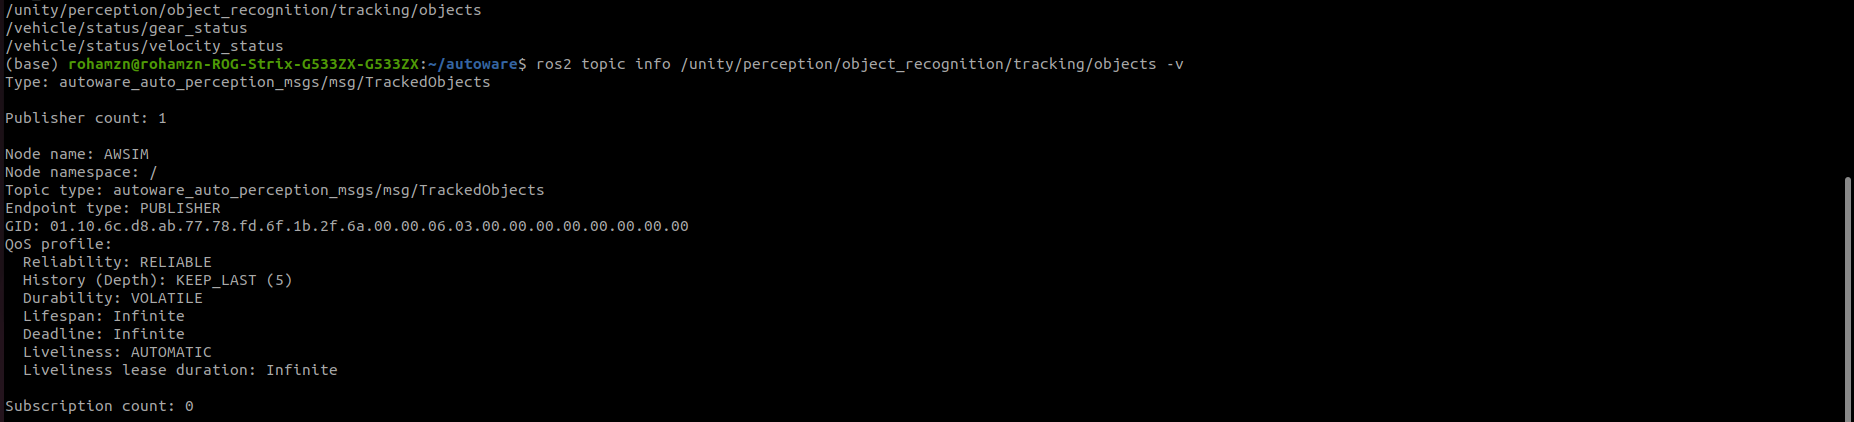
\includegraphics[width=1\linewidth]{figures/Unity_Publish_Tracked_Messages.png}
    \caption{مبحث منتشر شده پیام‌های ردیاب، توسط افزونه \lr{R2FU} در بستر \lr{Unity}}
    \label{fig:Unity_Publish_Tracked_Messages}
\end{figure}
در \cref{fig:Unity_Publish_Tracked_Messages} مشاهده می‌کنیم که پیام‌ها در حال انتشار شدن هستند و جنس آن‌ها نیز همان \lr{autoware\_auto\_perception\_msgs/msg/TrackedObjects} است.

\section{شبیه‌سازی ترافیک در شبیه‌ساز}
پس با موفقیت توانستیم پیام‌های گره ردیاب هم‌زمان چند جسم را با استفاده از \lr{Unity} بخوانیم. حال بایستی بتوانیم با پردازش این اطلاعات، ماشین‌هایی را در یک صحنه جدید در پروژه \lr{AWSIM}، پدیدار کنیم و سپس آن‌ها را حرکت دهیم.

\begin{figure}[h!]
    \centering
    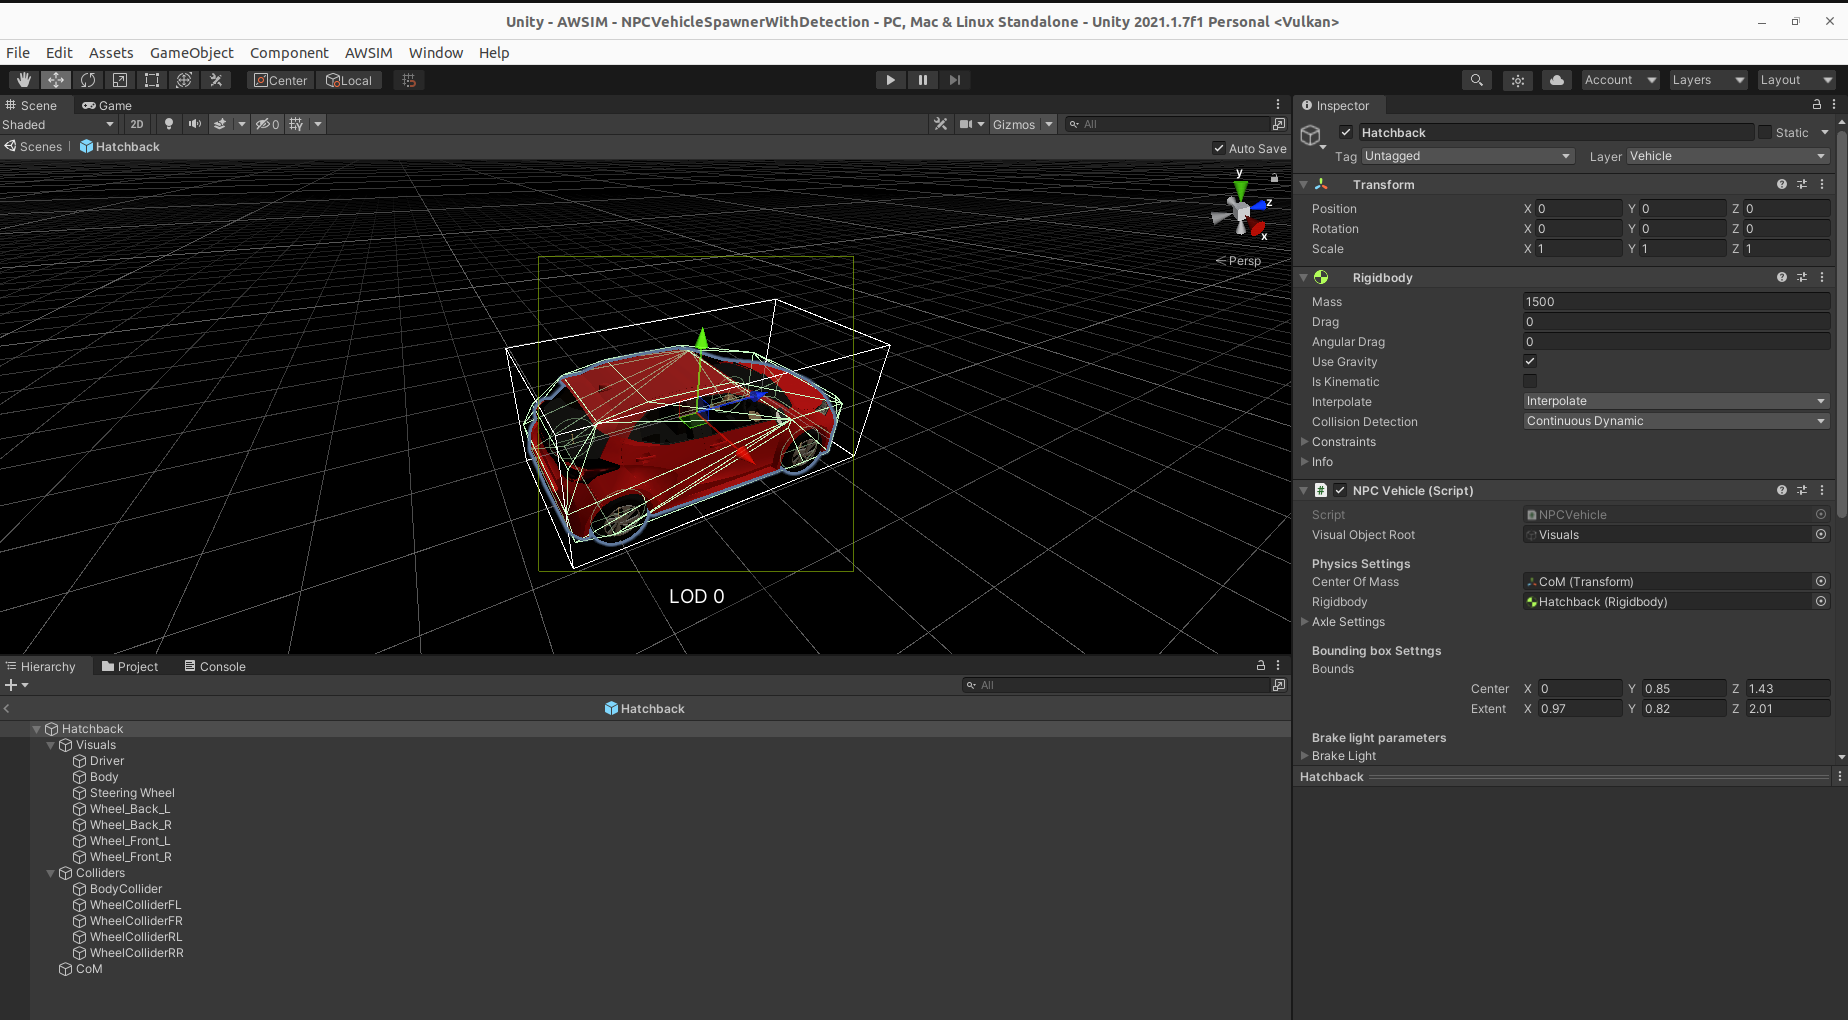
\includegraphics[width=1\linewidth]{figures/NPCVehicle_Prefab.png}
    \caption{یک خودروی نمونه پیش‌ساخته در پروژه \lr{AWSIM}}
    \label{fig:NPCVehicle_Prefab}
\end{figure}

بخاطر داریم که در این شبیه‌ساز، مولفه‌ای به نام مولفه شبیه‌ساز ترافیک\LTRfootnote{\lr{Traffic Simulator}} وجود دارد. در این مولفه، ماشین‌هایی با روش‌های سنتز ریاضی پدیدار می‌شوند که نام آن‌ها \lr{NPCVehicle} است. این ماشین‌ها جزو اشیاء بازی\LTRfootnote{\lr{Unity Game Object}} این شبیه‌ساز هستند و به همه آن‌ها به صورت پیش‌فرض، اسکریپتی مجهز می‌شود که وظیفه پیاده‌سازی رفتارها و کنترل‌های این ماشین‌ها را  بر عهده دارد. در \cref{fig:NPCVehicle_Prefab}، یکی از ماشین‌های پیش‌ساخته‌شده شبیه‌ساز ‌\lr{AWSIM} را مشاهده می‌کنیم. ملاحظه می‌شود که در بخش اسکریپ‌ها، اسکریپتی به نام \lr{NPCVehicle.cs} اضافه شده است.
\begin{figure}[h!]
    \centering
    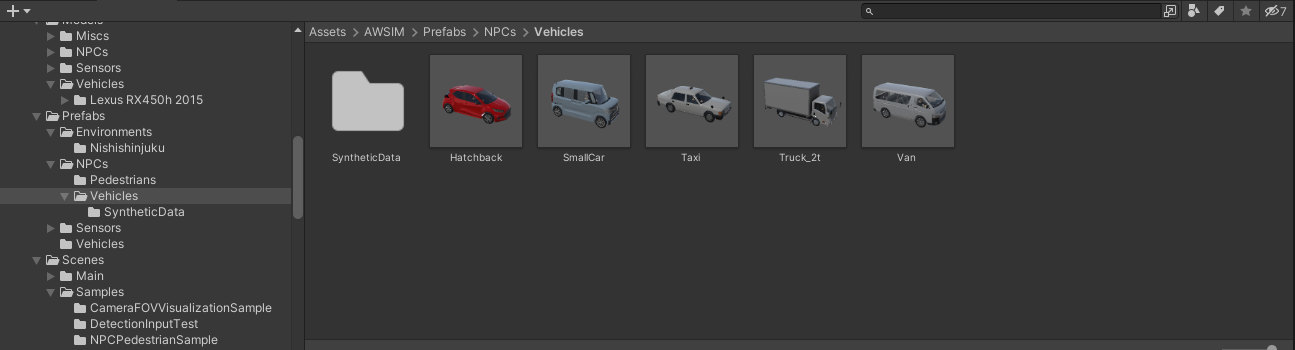
\includegraphics[width=1\linewidth]{figures/NPCVehicle_Prefabs.png}
    \caption{شبیه‌ساز ‌\lr{AWSIM}، چندین مدل خودرو برای ایجاد تنوع دارد.}
    \label{fig:NPCVehicle_Prefabs}
\end{figure}

شبیه‌ساز \lr{AWSIM}، در ساختار پوشه‌ای خود یک صحنه نمونه\LTRfootnote{\lr{Sample Scene}} دارد که نام آن \lr{NPCVehicalSample} است. 
\begin{figure}[h!]
    \centering
    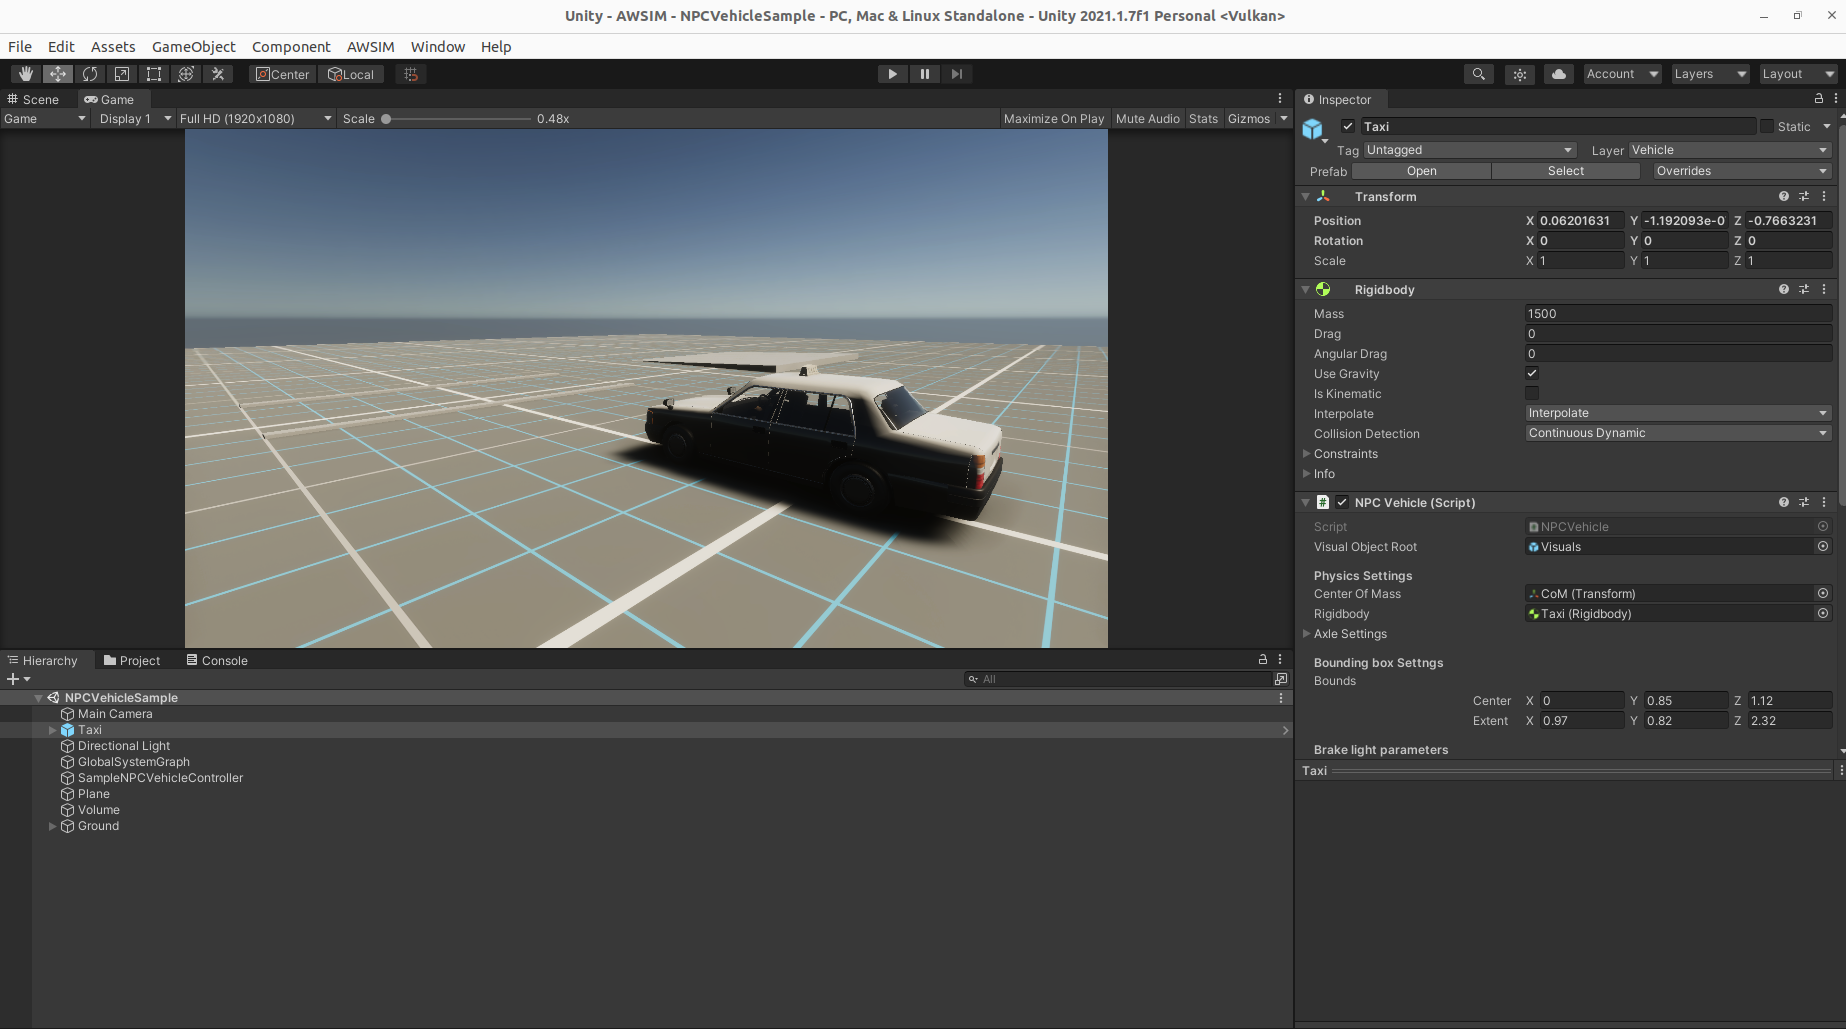
\includegraphics[width=1\linewidth]{figures/NPCVehicleSample.png}
    \caption{صحنه نمونه یک خودرو از جنس \lr{NPCVehicle}}
    \label{fig:NPCVehicleSample}
\end{figure}
\cref{fig:NPCVehicleSample} این صحنه را نشان می‌دهد. همانطور که مشاهده می‌کنیم، یک خودروی تاکسی با اسکریپت \lr{NPCVehicle} در صحنه وجود دارد. با اجرای این صحنه نمونه، خودروی تاکسی شروع به حرکت می‌کند و تمام حالات حرکتی آن بررسی می‌شود. این دستورات اعمال شده به خودروی تاکسی، توسط اسکریپتی دیگر به نام \lr{SampleNPCVehicleController} داده می‌شوند.

\begin{figure}[h!]
    \centering
    \begin{latin}
        \begin{lstlisting}[style=codecs]
IEnumerator Routine()
{
    Debug.Log("--- Start control NPCVehicle ---");
    Debug.Log("Straight");
    yield return UpdatePosAndRot(5f, 3f, 0f);
    Debug.Log("Turn right");
    yield return UpdatePosAndRot(13.4f, 3f, 20f);
    Debug.Log("Straight");
    yield return UpdatePosAndRot(2f, 3f, 0f);
    Debug.Log("Left turn signal");

    npcVehicle.SetTurnSignalState(NPCVehicle.TurnSignalState.LEFT);
    yield return new WaitForSeconds(2f);
    Debug.Log("Right turn signal");

    npcVehicle.SetTurnSignalState(NPCVehicle.TurnSignalState.RIGHT);
    yield return new WaitForSeconds(2f);
    Debug.Log("Hazard signal");

    npcVehicle.SetTurnSignalState(NPCVehicle.TurnSignalState.HAZARD);
    Debug.Log("Back Right");
    yield return UpdatePosAndRot(3f, -2f, -30f);
    Debug.Log("Back");
    yield return UpdatePosAndRot(2f, -2f, 0f);
    Debug.Log("--- End control NPC Vehicle ---");
}
        \end{lstlisting}
    \end{latin}
    \caption{بخشی از کد \lr{NPCVehicleController} که به خودروهای \lr{NPCVehicle} دستورهای حرکتی متنوع می‌دهد.}
    \label{fig:NPCVehicleController1}
\end{figure}


\begin{figure}[h!]
    \centering
    \begin{latin}
        \begin{lstlisting}[style=codecs]
IEnumerator UpdatePosAndRot(float duration, float speed, float yawSpeed, bool validatePose = true)
{
    var startTime = Time.fixedTime;
    yield return new WaitForFixedUpdate();
    while (Time.fixedTime - startTime < duration)
    {
        var euler = currentRotation.eulerAngles;
        currentRotation = Quaternion.Euler(euler.x, euler.y + yawSpeed * Time.fixedDeltaTime, euler.z);
        currentPosition += currentRotation * Vector3.forward * speed * Time.fixedDeltaTime;
        npcVehicle.SetRotation(currentRotation);
        npcVehicle.SetPosition(currentPosition);
        yield return new WaitForFixedUpdate();
    }
}
        \end{lstlisting}
    \end{latin}
    \caption{بخشی از کد \lr{NPCVehicleController} که در آن نحوه شبیه‌سازی حرکت خودروها نمایش داده شده است.}
    \label{fig:NPCVehicleController2}
\end{figure}

\cref{fig:NPCVehicleController1}، کد مربوط به این حرکات خودروی تاکسی را نشان می‌دهد. مشاهده می‌کنیم که این دستورات توسط کوروتین‌ها\LTRfootnote{\lr{Coroutine}} اجرا می‌شوند که باعث اجرای موازی دستورات می‌شود، تا باعث انسداد در خط لوله اجرایی موتور \lr{Unity} نشود. حال به بررسی تابع \lr{UpdatePosAndRot} می‌پردازیم. \cref{fig:NPCVehicleController2}، این کد را نشان می‌دهد. مشاهده می‌کنیم که برای حرکت خودرو، مدت زمان حرکت، سرعت‌ خطی، و سرعت زاویه‌ای به عنوان ورودی گرفته می‌شود. سپس با اعمال فرمول‌های ساده سینماتیک، مختصات جدید خودرو را در هر واحد زمانی از شبیه‌ساز، محاسبه می‌کند. توابع \lr{SetRotation} و \lr{SetPosition}، از دستورات اسکریپت \lr{NPCVehicle} هستند که با توجه به فیزیک خودرو، آن را به زاویه و مختصات خواسته شده حرکت می‌دهد.

\subsection{ایجاد صحنه جدید}
\begin{figure}[h!]
    \centering
    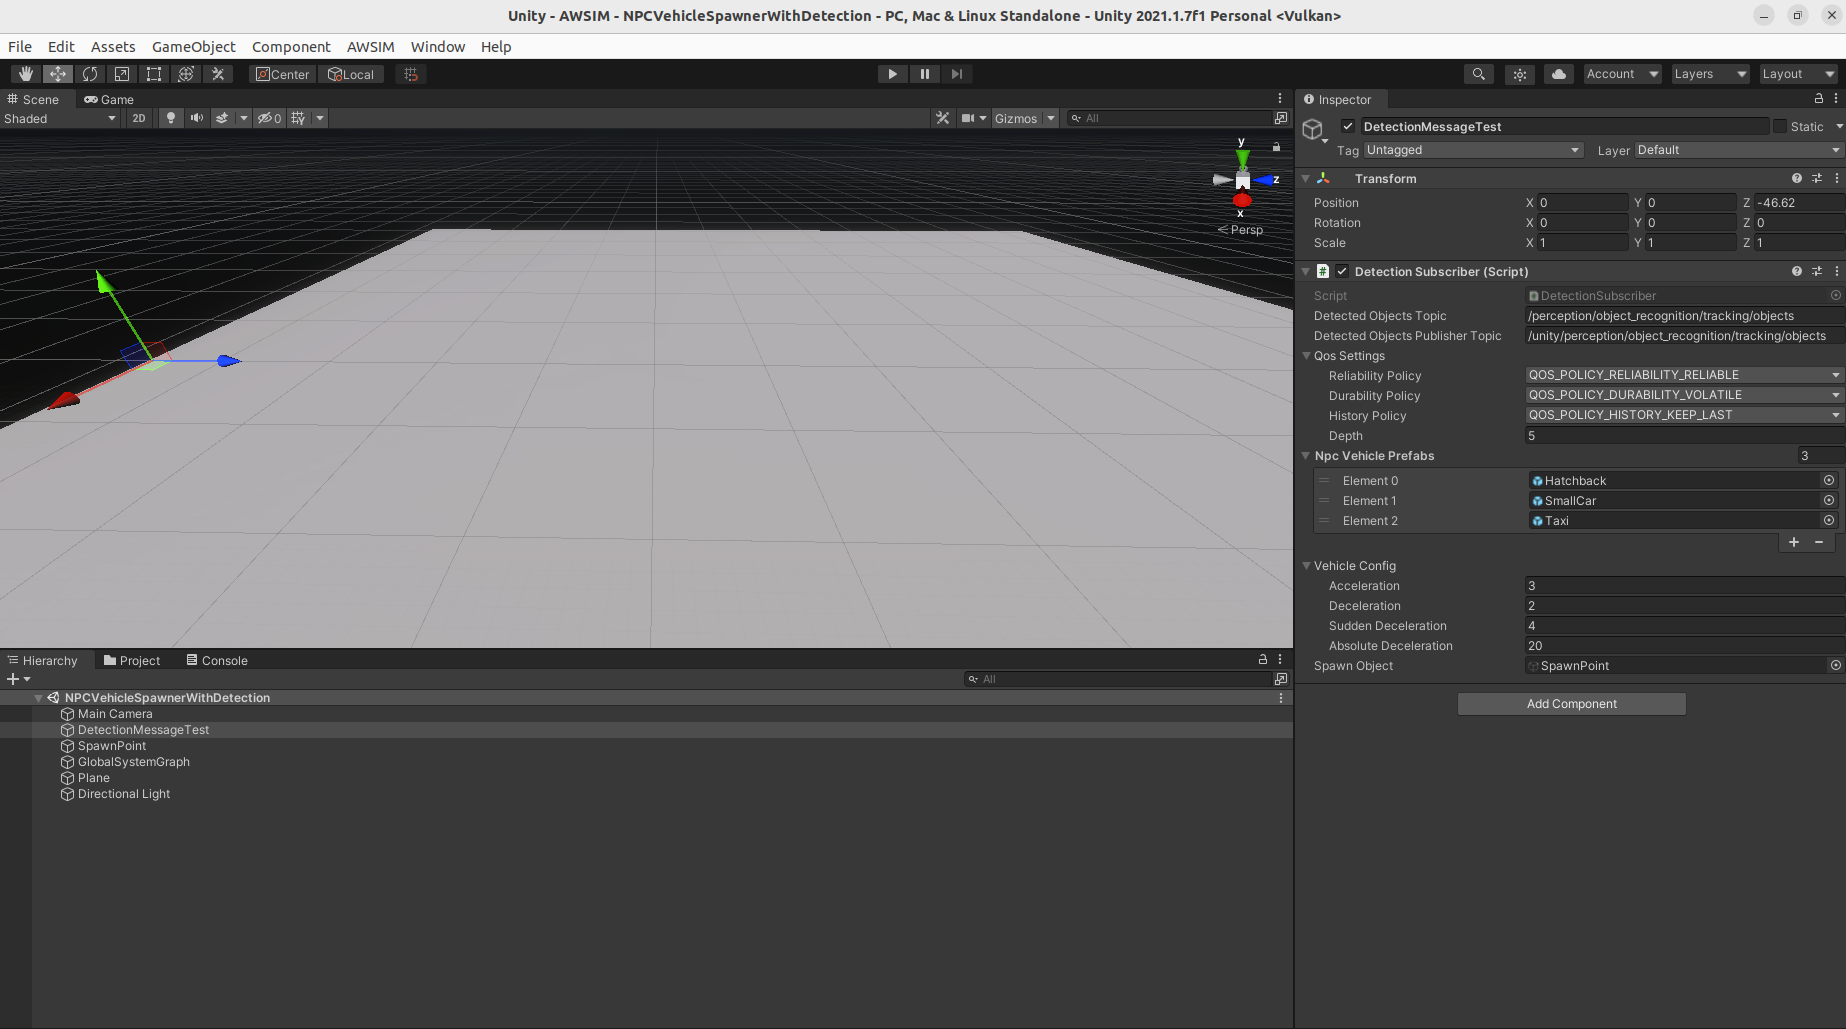
\includegraphics[width=1\linewidth]{figures/NPCVehicleSpawnerWithDetectionScene.png}
    \caption{صحنه جدید ساخته شده برای شبیه‌سازی ترافیک}
    \label{fig:NPCVehicleSpawnerWithDetectionScene}
\end{figure}
قبل از آنکه بتوانیم از اسکریپت حرکت دادن خودروهای \lr{NPCVehicle} استفاده کنیم، بایستی یک صحنه جدید بسازیم.
سپس در این صحنه یک زمین صاف قرار دهیم و شئ بازی‌ای اضافه کنیم که مسئولیت اشتراک‌گیری از مبحث پیام ردیاب را دارد، سپس با توجه به درصد احتمال وجود جسم و برچسب آن‌ها، خودرو‌ها را در صحنه شبیه‌سازی پدیدار کند. 
\cref{fig:NPCVehicleSpawnerWithDetectionScene}، این صحنه جدید را نشان می‌دهد. ملاحظه می‌شود که داخل سلسه‌ مراتب\LTRfootnote{\lr{Hierarchy}} این صحنه، شئ بازی‌ای به نام \lr{DetectionMessageTest} ساخته شده است. به این شئ، اسکریپتی متصل شده است که اشتراکی در مبحث اجسام ردیابی شده دارد. 
\begin{figure}[h!]
    \centering
    \begin{latin}
        \begin{lstlisting}[style=codecs]
trackedObjectsSubscriber
= SimulatorROS2Node.CreateSubscription<autoware_auto_perception_msgs.msg.TrackedObjects>(
detectedObjectsTopic, msg =>
{
    trackedObjectsPublisher.Publish(msg);
    currentFrameVehicles = new List<String>();
    foreach (autoware_auto_perception_msgs.msg.TrackedObject obj in msg.Objects){
        if (obj.Classification[0].Label == car && obj.Existence_probability >= 0.3){
            string uuid = BitConverter.ToString(obj.Object_id.Uuid).Replace("-", "");
            currentFrameVehicles.Add(uuid);
            if (detectedVehicles.ContainsKey(uuid)){
                detectedVehicles[uuid] = obj;
                continue;
            }
            Debug.Log("New Object ID: " + uuid);
        
            detectedVehicles.Add(uuid, obj);
        }
    }
}, qos);
        \end{lstlisting}
    \end{latin}
    \caption{بخشی از کد \lr{DetectionSubscriber}}
    \label{fig:DetectionSubscriber1}
\end{figure}

در \cref{fig:DetectionSubscriber1}، بخشی از کد \lr{DetectionSubscriber} را مشاهده می‌کنیم، که وظیفه فیلتر کردن اجسام ردیابی شده را دارد. این فیلتر، براساس درصد احتمال وجود تخمین زده اجسام کار می‌کند که توسط ردیاب \lr{Autoware}، محاسبه شده است. حد آستانه این فیلتر، \%۳۰ در نظر گرفته شده است.
\begin{figure}[h!]
    \centering
    \begin{latin}
        \begin{lstlisting}[style=codecs]
IEnumerator Routine(string vehicleID)
{
    Vector3 spawnPosition = new Vector3((float)-detectedVehicles[vehicleID].Kinematics.Pose_with_covariance.Pose.Position.Y, 0f, (float)detectedVehicles[vehicleID].Kinematics.Pose_with_covariance.Pose.Position.X);
    Quaternion rotation = new Quaternion(0f, (float)-detectedVehicles[vehicleID].Kinematics.Pose_with_covariance.Pose.Orientation.Z, 0f, (float)detectedVehicles[vehicleID].Kinematics.Pose_with_covariance.Pose.Orientation.W);
    NPCVehicle vehicle = npcVehicleSpawner.Spawn(npcVehicleSpawner.GetRandomPrefab(), SpawnIdGenerator.Generate(), spawnPosition, rotation, spawnObject.transform);
    npcVehicles.Add(vehicleID, vehicle);
    // ...
}
        \end{lstlisting}
    \end{latin}
    \caption{بخشی از کوروتین کد \lr{DetectionSubscriber}}
    \label{fig:DetectionSubscriber2}
\end{figure}
شناسه خودروهایی که از فیلتر عبور کنند، به آرایه‌ای به نام \lr{detectedVehicles} اضافه می‌شوند. سپس کوروتینی به این جسم تعلق می‌گیرد که اقدام به پدیدار کردن خودروی ردیابی شده  و حرکت دادن آن می‌کند. برای این کار، مختصات تشخیص داده شده از جسم، به همراه جهت آن را از پیام ردیابی مربوط به آن جسم استخراج می‌کنیم و با تابعی به نام \lr{npcVehicleSpawner} آن را نسبت به شئ بازی‌ای به نام \lr{Spawn Point}، که فرض می‌شود مختصات لایدار است، پدیدار می‌کنیم.

برای حرکت دادن ماشین‌های حاضر در صحنه، در کوروتین متعلق به جسم، شروع به دریافت مختصات و جهت‌های خودرو می‌کنیم تا زمانی که دیگر خودرویی با این شناسه، در آرایه خودروهای تشخیص داده شده جدید وجود نداشته باشد. سپس این جهت‌ها و مختصات جدید را به توابع حرکتی (که در \cref{fig:NPCVehicleController2} مشاهده کردیم) می‌دهیم تا خودروی \lr{NPCVehicle}، به سمت مختصات جدید حرکت کند.

\begin{figure}[h!]
    \centering
    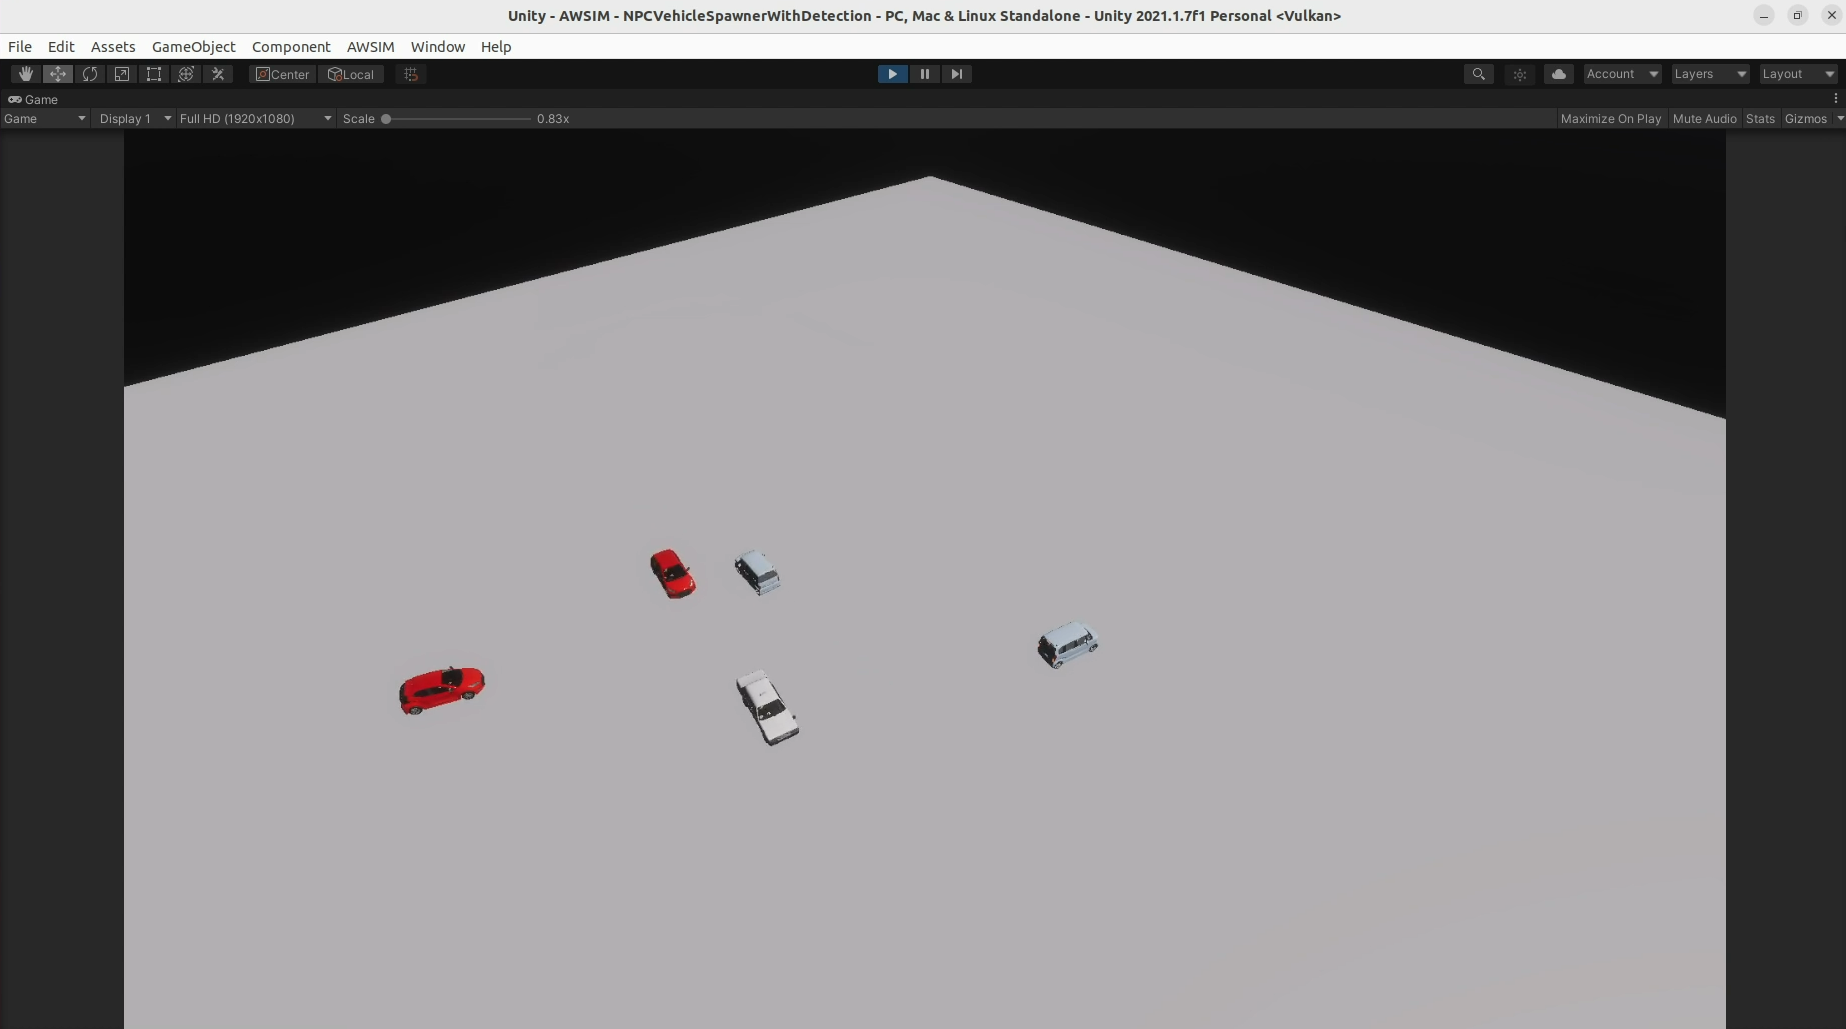
\includegraphics[width=1\linewidth]{figures/NPCVehicleSimulation.png}
    \caption{شبیه‌سازی موفق از ترافیک مشاهده شده در داده نمونه}
    \label{fig:NPCVehicleSpawnerWithDetectionScene}
\end{figure}

همانطور که از \cref{fig:NPCVehicleSpawnerWithDetectionScene} معلوم است، مشاهده می‌کنیم که خودروها به درستی پدیدار شده‌اند و حرکت می‌کنند! در \cref{fig:SimulationProcess} نیز نگاهی به پروسه طی شده در این سناریو می‌اندازیم.

\begin{figure}[h!]
    \centering
    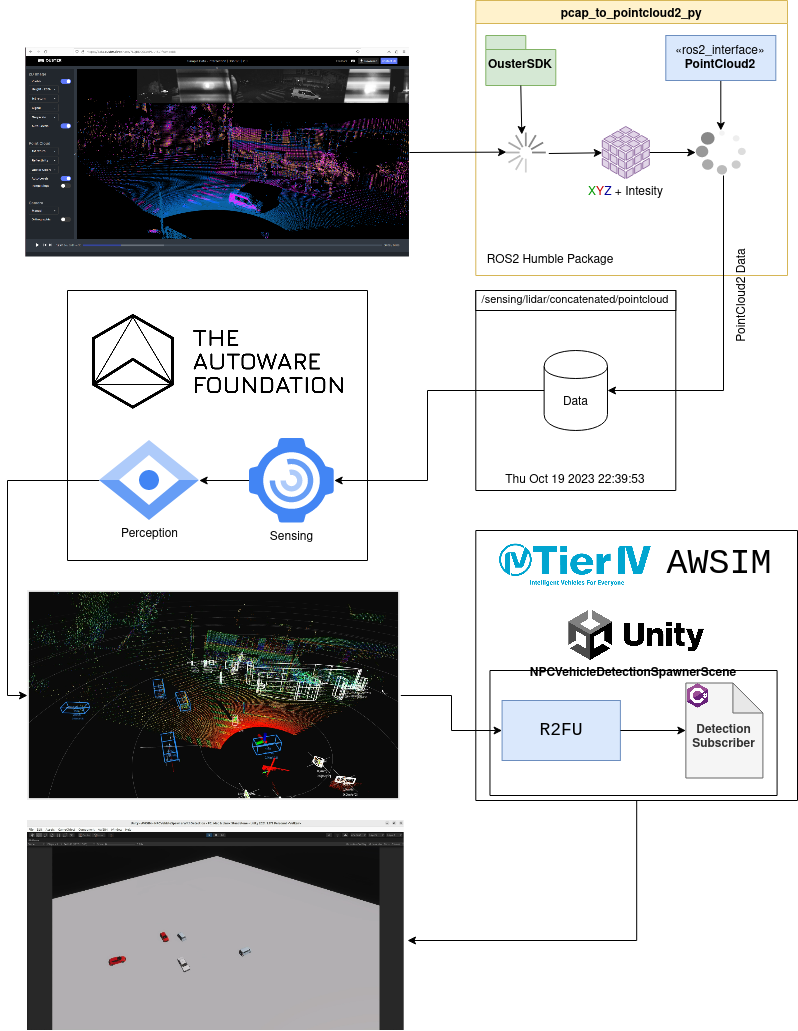
\includegraphics[width=1\linewidth]{figures/SimulationProcess.png}
    \caption{پروسه شبیه‌سازی بلادرنگ سناریو اول با داده نمونه}
    \label{fig:SimulationProcess}
\end{figure}

\subsection{نتیجه‌گیری سناریو اول}
مشاهده کردیم که در این پژوهش، به شبیه‌سازی بلادرنگ خودروها با استفاده از داده‌ نمونه گرفته شده از \lr{Ouster}، رسیدیم. پس می‌توان با قاطعیت گفت که سناریو دوم امکان پذیر است.
البته لازم به ذکر است که از آنجایی که تشخیص‌دهنده دقت \%۱۰۰ ندارد، شبیه‌سازی با عیب‌ و نقص‌هایی روبرو خواهد شد، اما نتیجه گرفته شده امیدمان را نسبت به پیاده‌سازی دوقلویی دیجیتال با دقت بالای \%۹۰، افزایش می‌دهد.

\section{سناریو دوم: داده‌برداری از منطقه خیابان رشت و طراحی سه‌بعدی}
با اطمینان از اینکه شبیه‌ساز با هر داده ابر نقطه‌ای کار می‌کند، عملیات گرفتن مجوز از دانشگاه و داده‌برداری از خیابان رشت، آغاز شد.

\subsection{داده‌برداری از خیابان رشت}
خیابان رشت، خیابانی است که در ضلع شمالی دانشگاه امیرکبیر واقع شده است و حجم زیادی تردد را همیشه به همراه خود دارد. \cref{fig:Amirkabir_Campus}،‌  محوطه دانشگاه امیرکبیر را نشان می‌دهد.
\begin{figure}[h!]
    \centering
    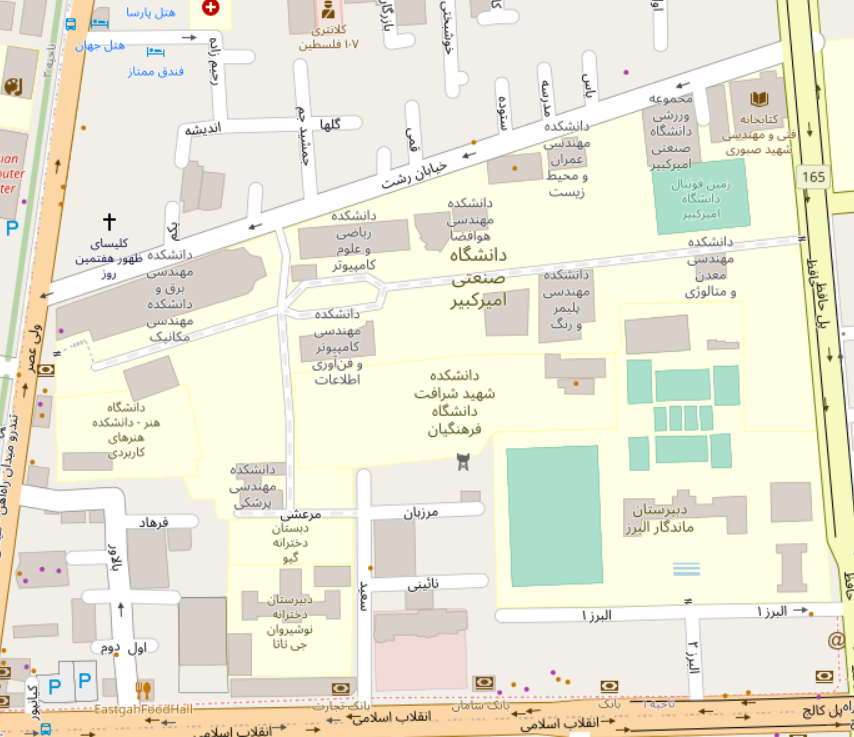
\includegraphics[width=0.8\linewidth]{figures/Amirkabir_Campus.png}
    \caption{نقشه پردیس دانشگاه امیرکبیر}
    \label{fig:Amirkabir_Campus}
\end{figure}

\begin{figure}[h!]
    \begin{minipage}{0.5\textwidth}
        \centering
        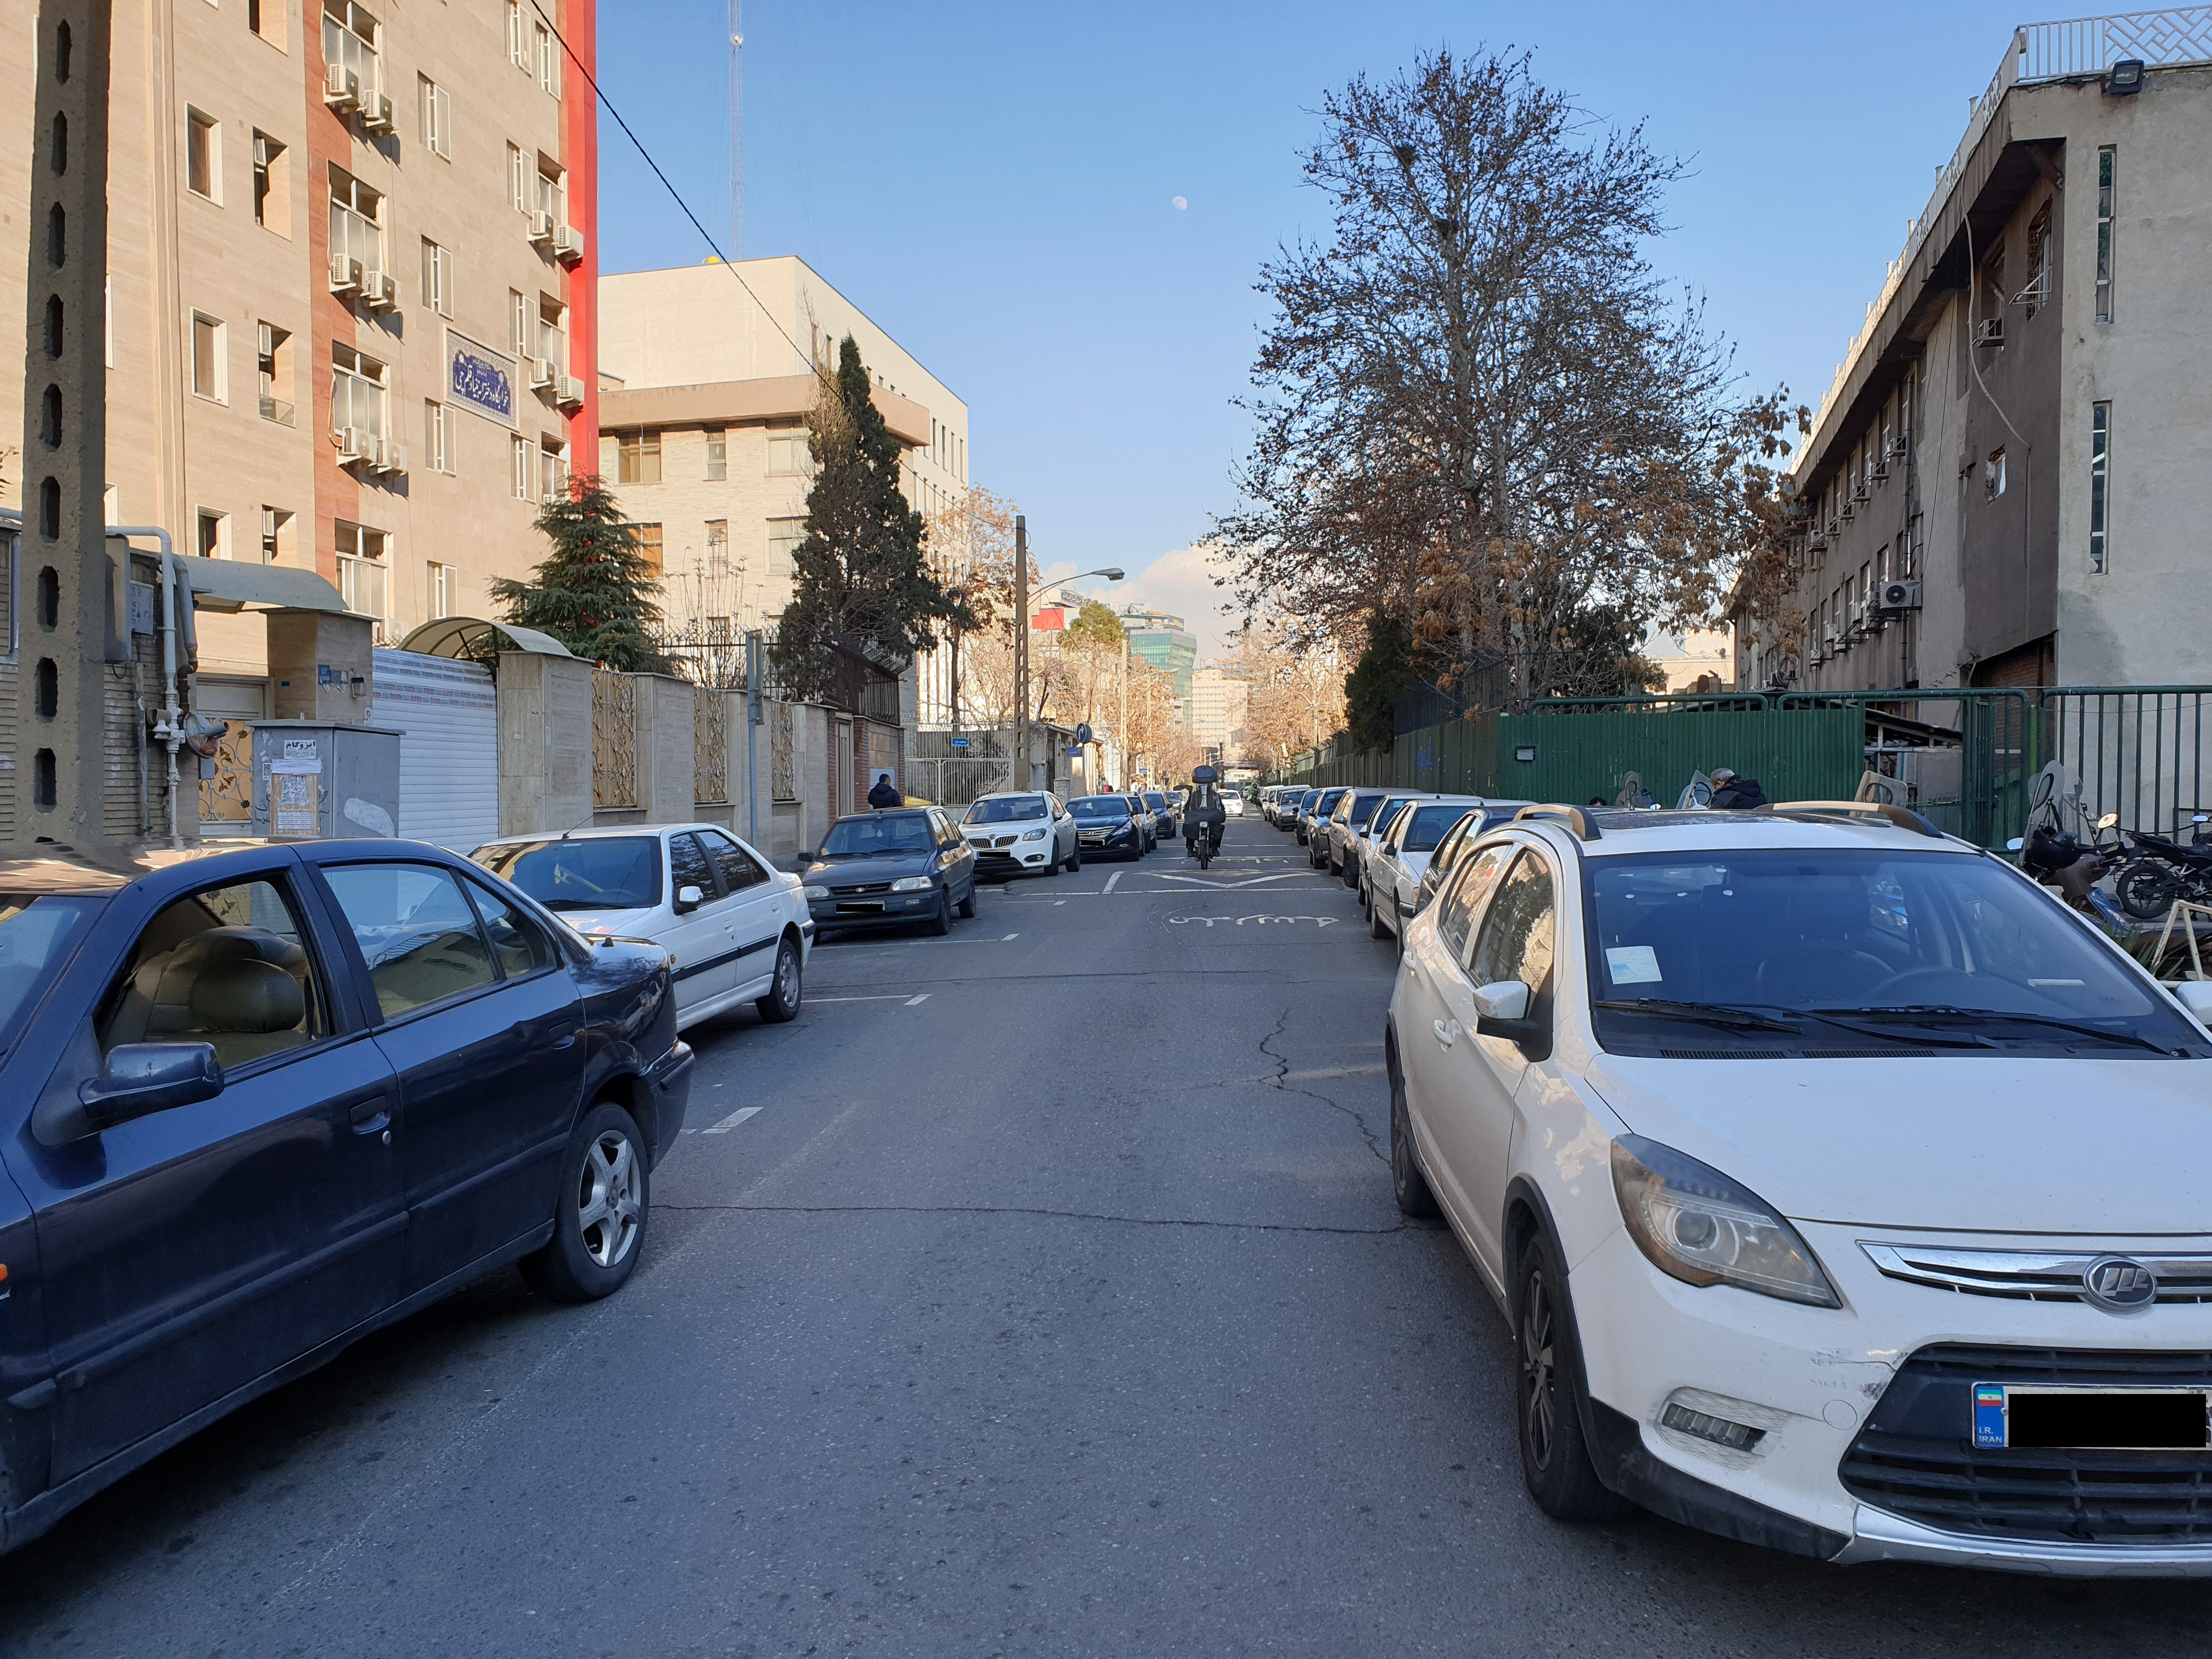
\includegraphics[width=1\linewidth]{figures/Rasht_Picture1.jpg}
    \end{minipage}
    \hspace{0.3cm}
    \begin{minipage}{0.5\textwidth}
        \centering
        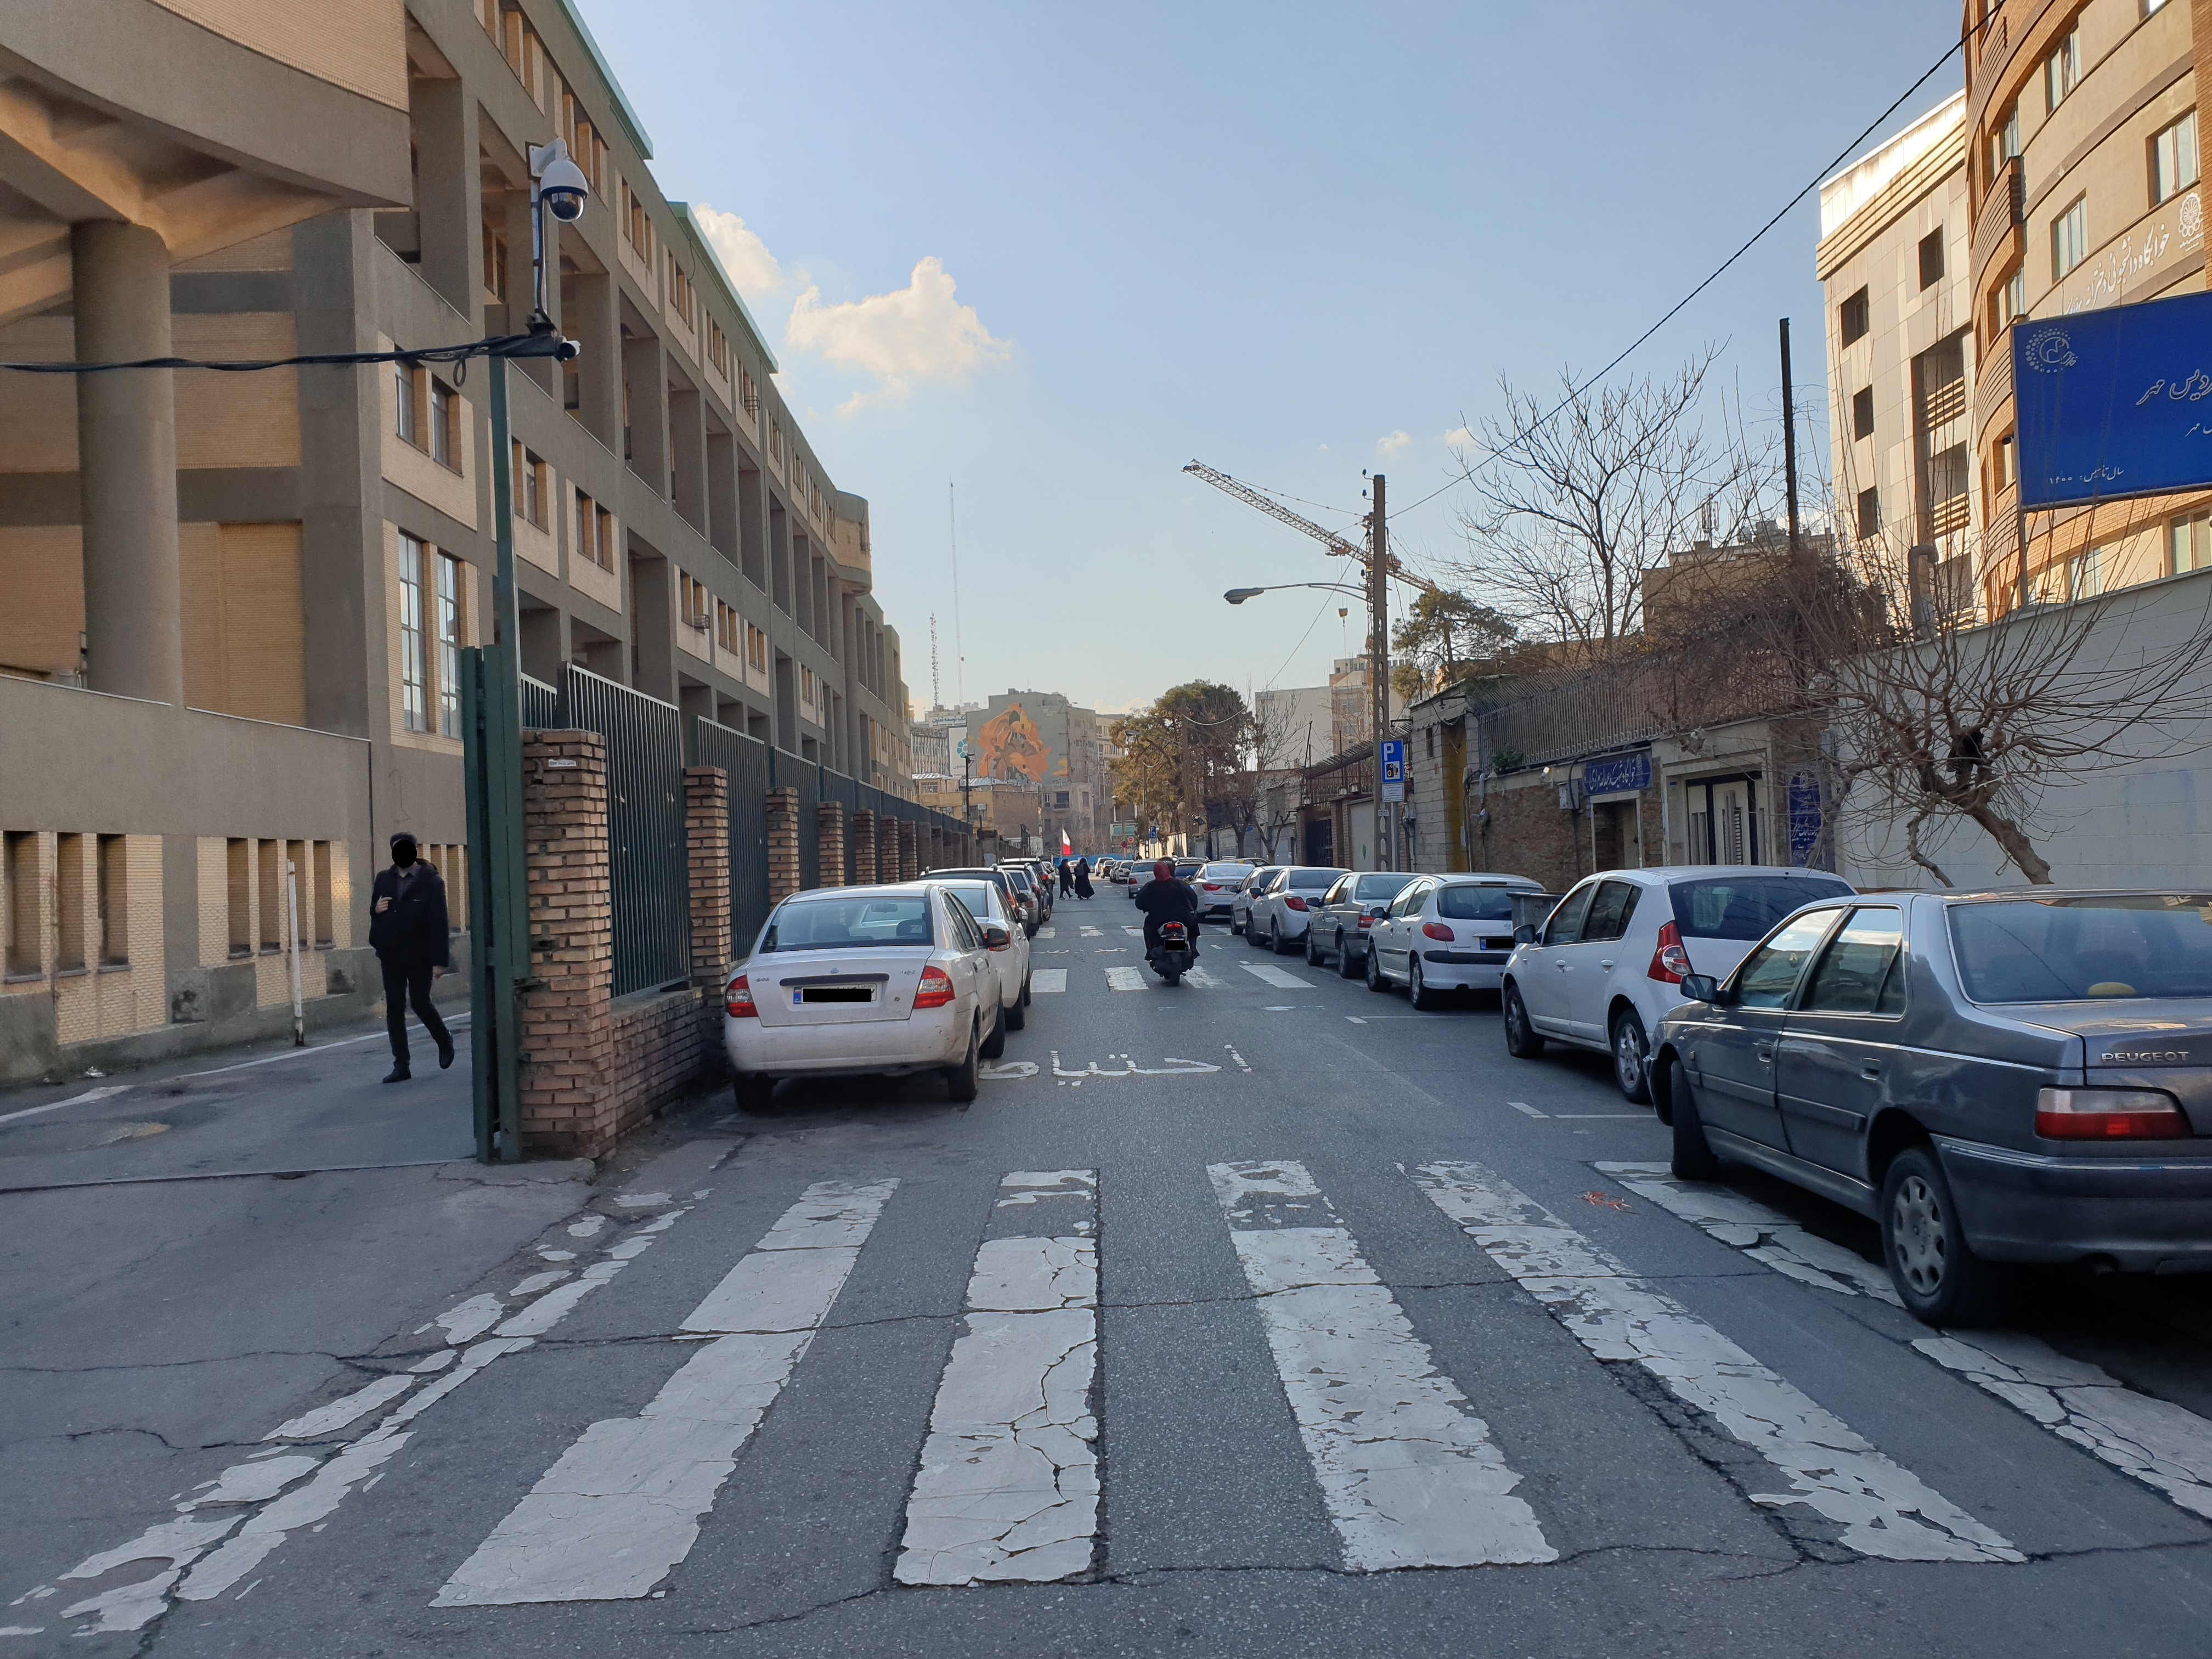
\includegraphics[width=1\linewidth]{figures/Rasht_Picture2.jpg}
    \end{minipage}
    \begin{center}
        \caption{تصاویر خیابان رشت از زاویه دید درب رشت}
    \end{center}
    \label{fig:Rasht_Pictures}
\end{figure} 

در این داده‌برداری، از سنسور لایدار \lr{OS1:64} استفاده می‌شود و دوربین فیلم‌برداری نیز دوربین موبایل است. محلی که سنسورها مستقر شدند، پشت بام خیابان رشت بود. \cref{fig:Rasht_Roof_Proposal}، منطقه پیشنهادی را نشان می‌دهد. 

 \begin{figure}[h!]
    \centering
    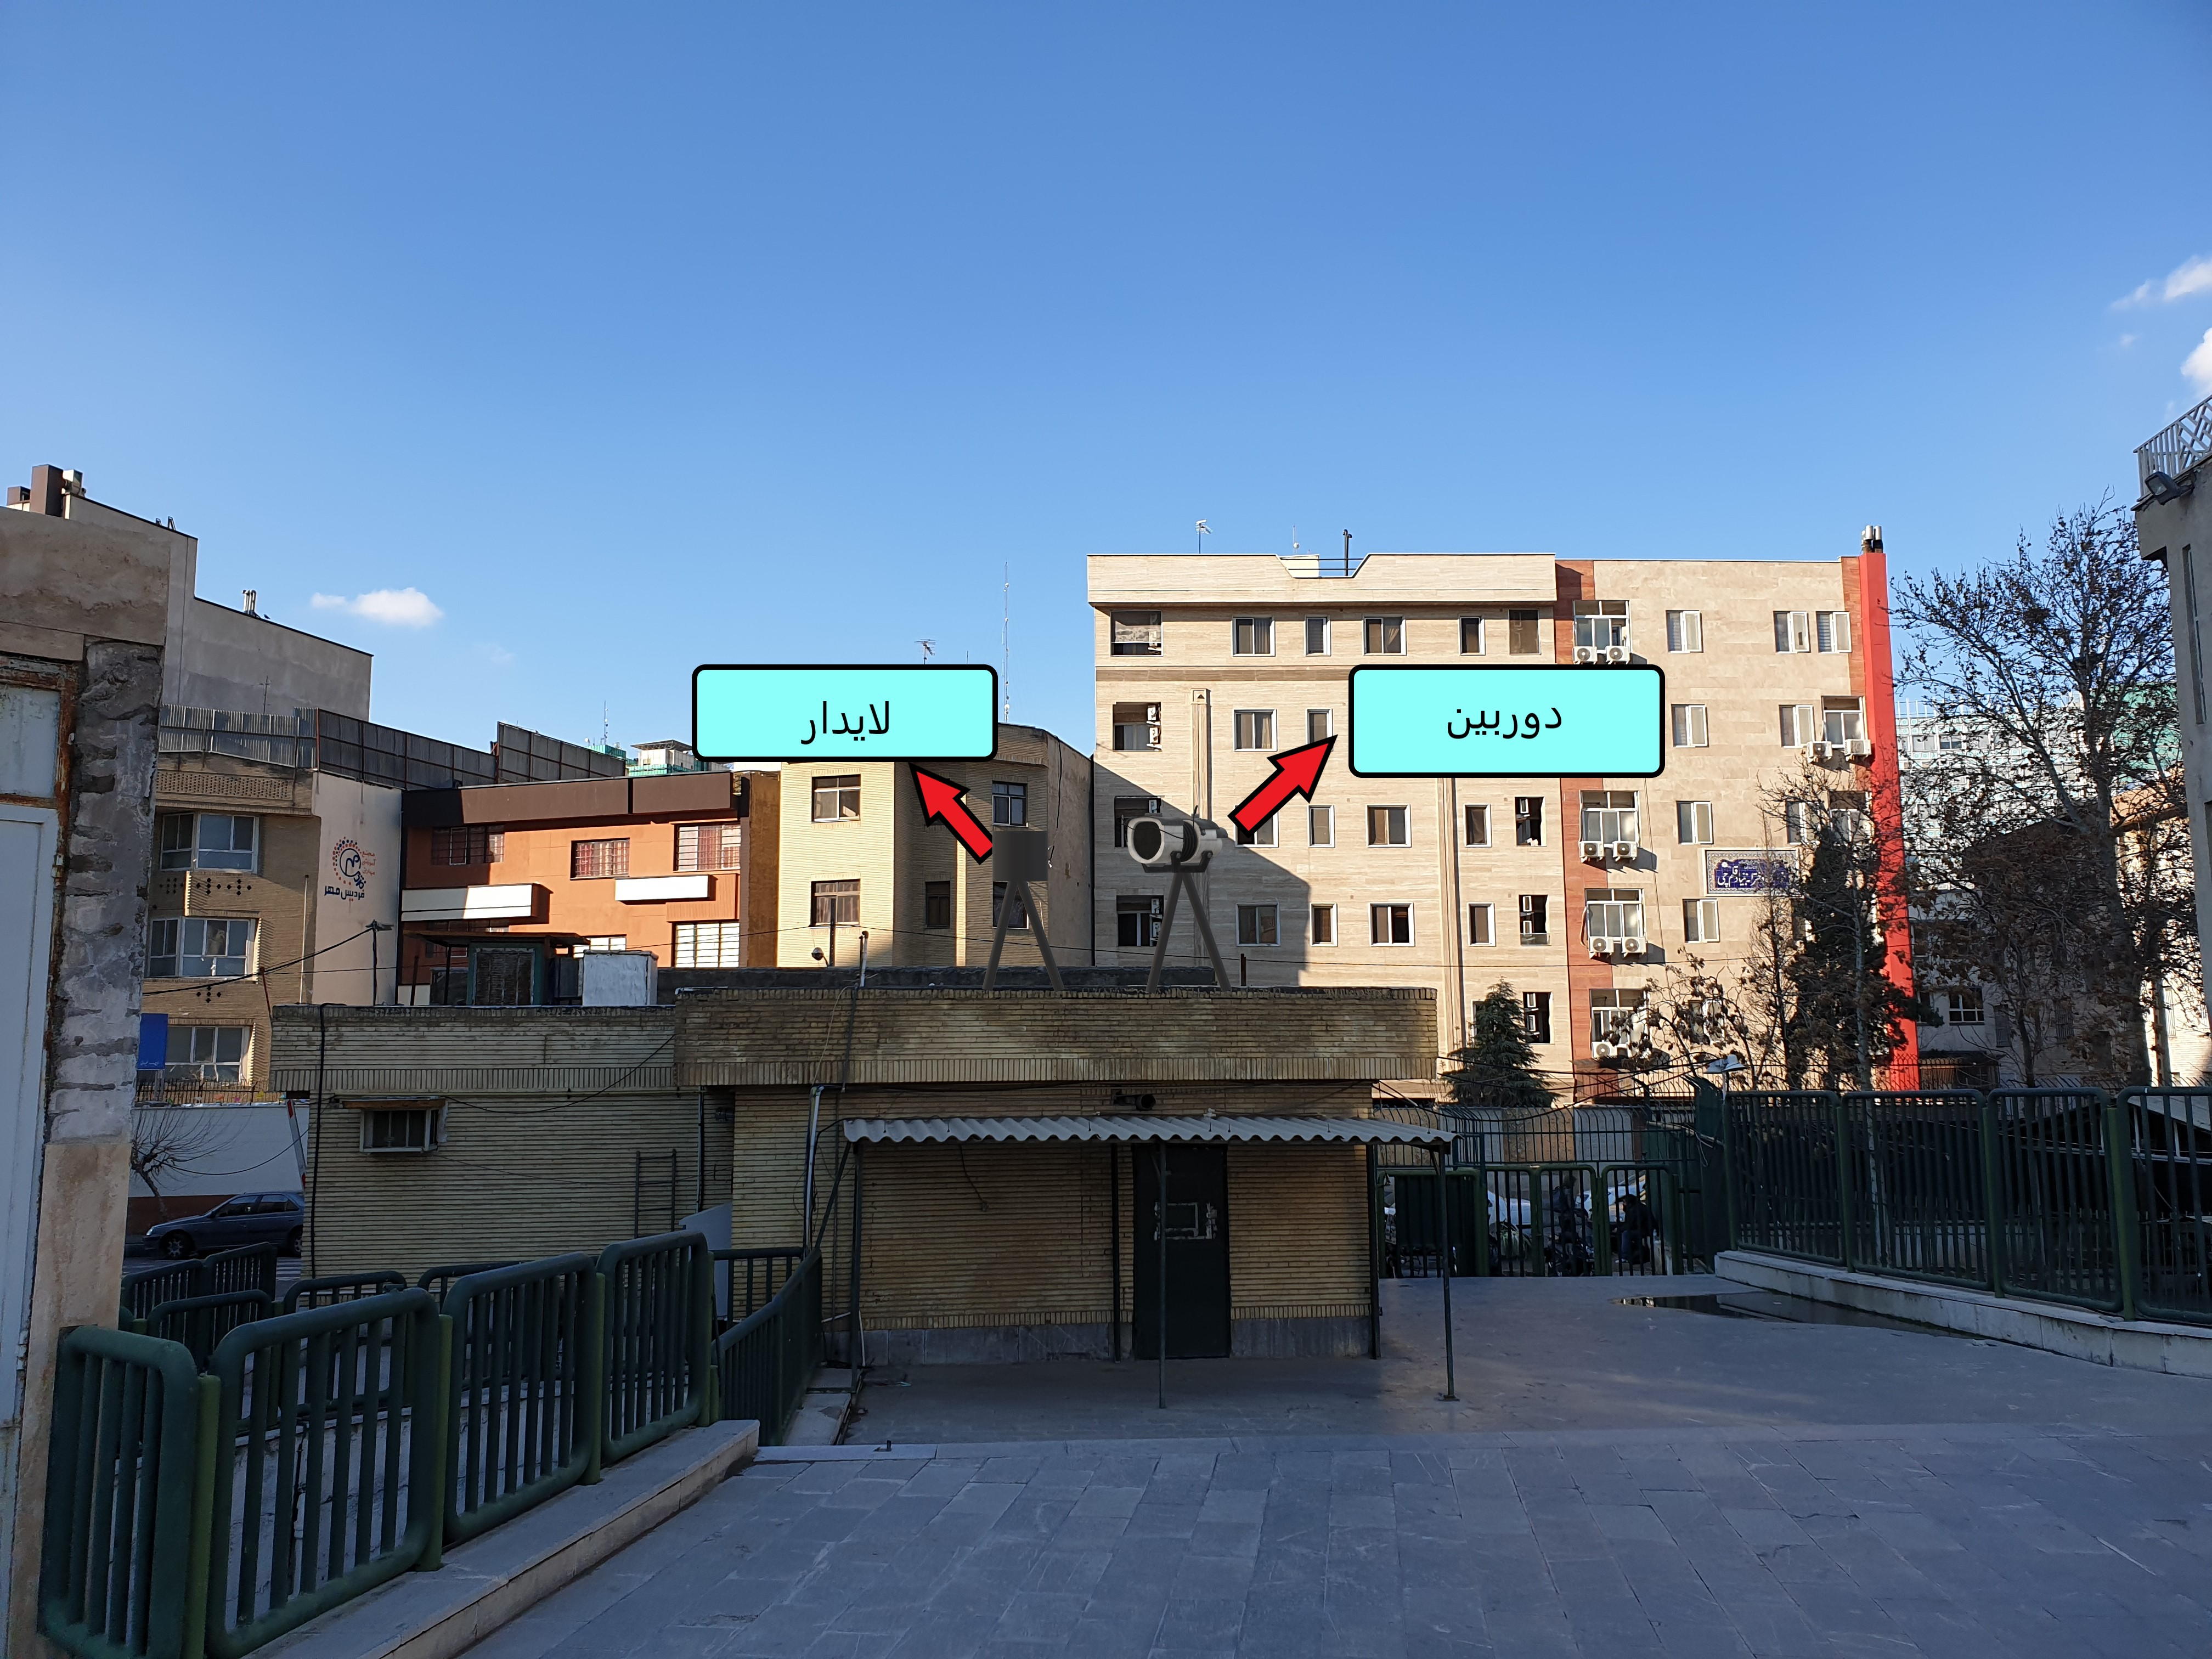
\includegraphics[width=1\linewidth]{figures/rasht_edited.jpg}
    \caption{محل پیشنهادی داده‌برداری}
    \label{fig:Rasht_Roof_Proposal}
\end{figure}

برای عملیات داده برداری، از یک سیم رابط ۱۰ متری، سه‌پایه برای لایدار، لپ‌تاپ برای ضبط داده، لایدار، دوربین موبایل و یک نردبان استفاده شد. برای ضبط داده نیز از نرم‌افزار \lr{Ouster Studio} استفاده شد.
\\

\begin{figure}[h!]
    \begin{minipage}{0.5\textwidth}
        \centering
        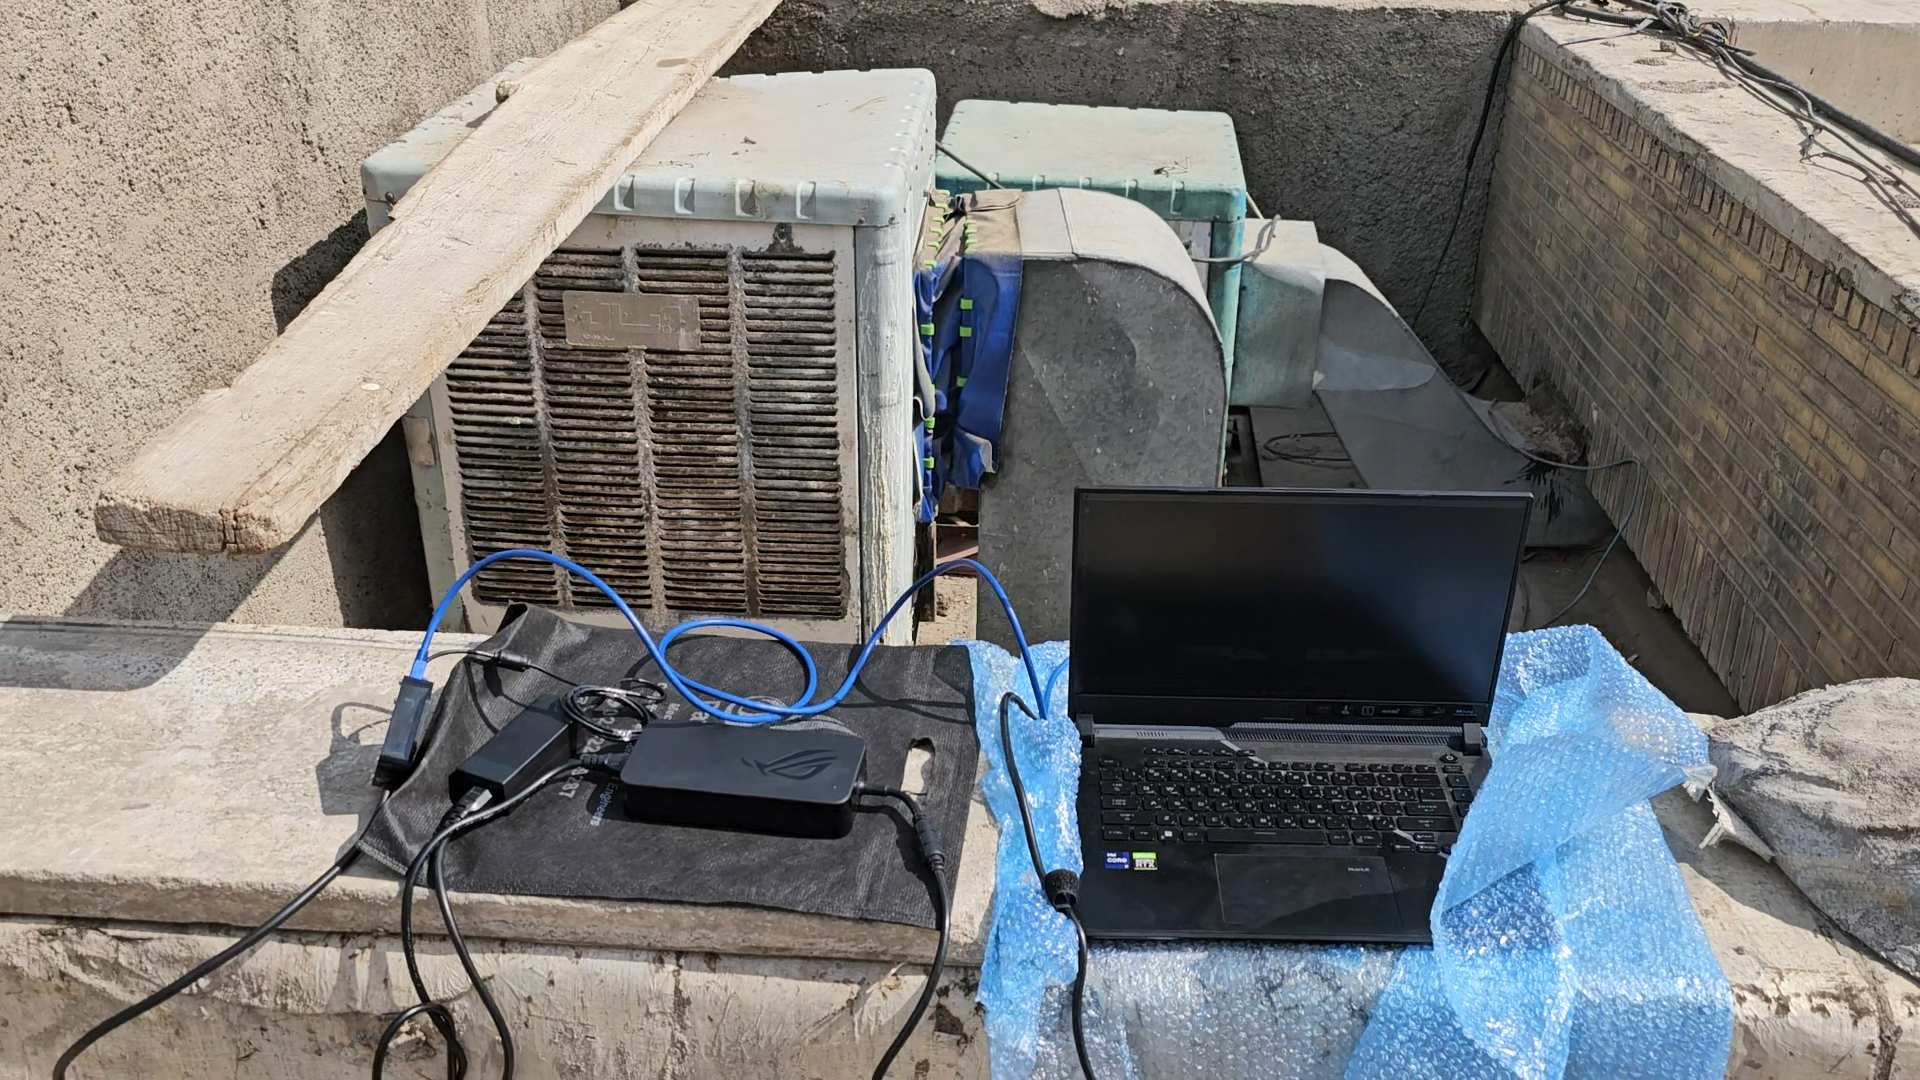
\includegraphics[width=1\linewidth]{figures/Lidar_Data_Acquisition1.png}
    \end{minipage}
    \hspace{0.3cm}
    \begin{minipage}{0.5\textwidth}
        \centering
        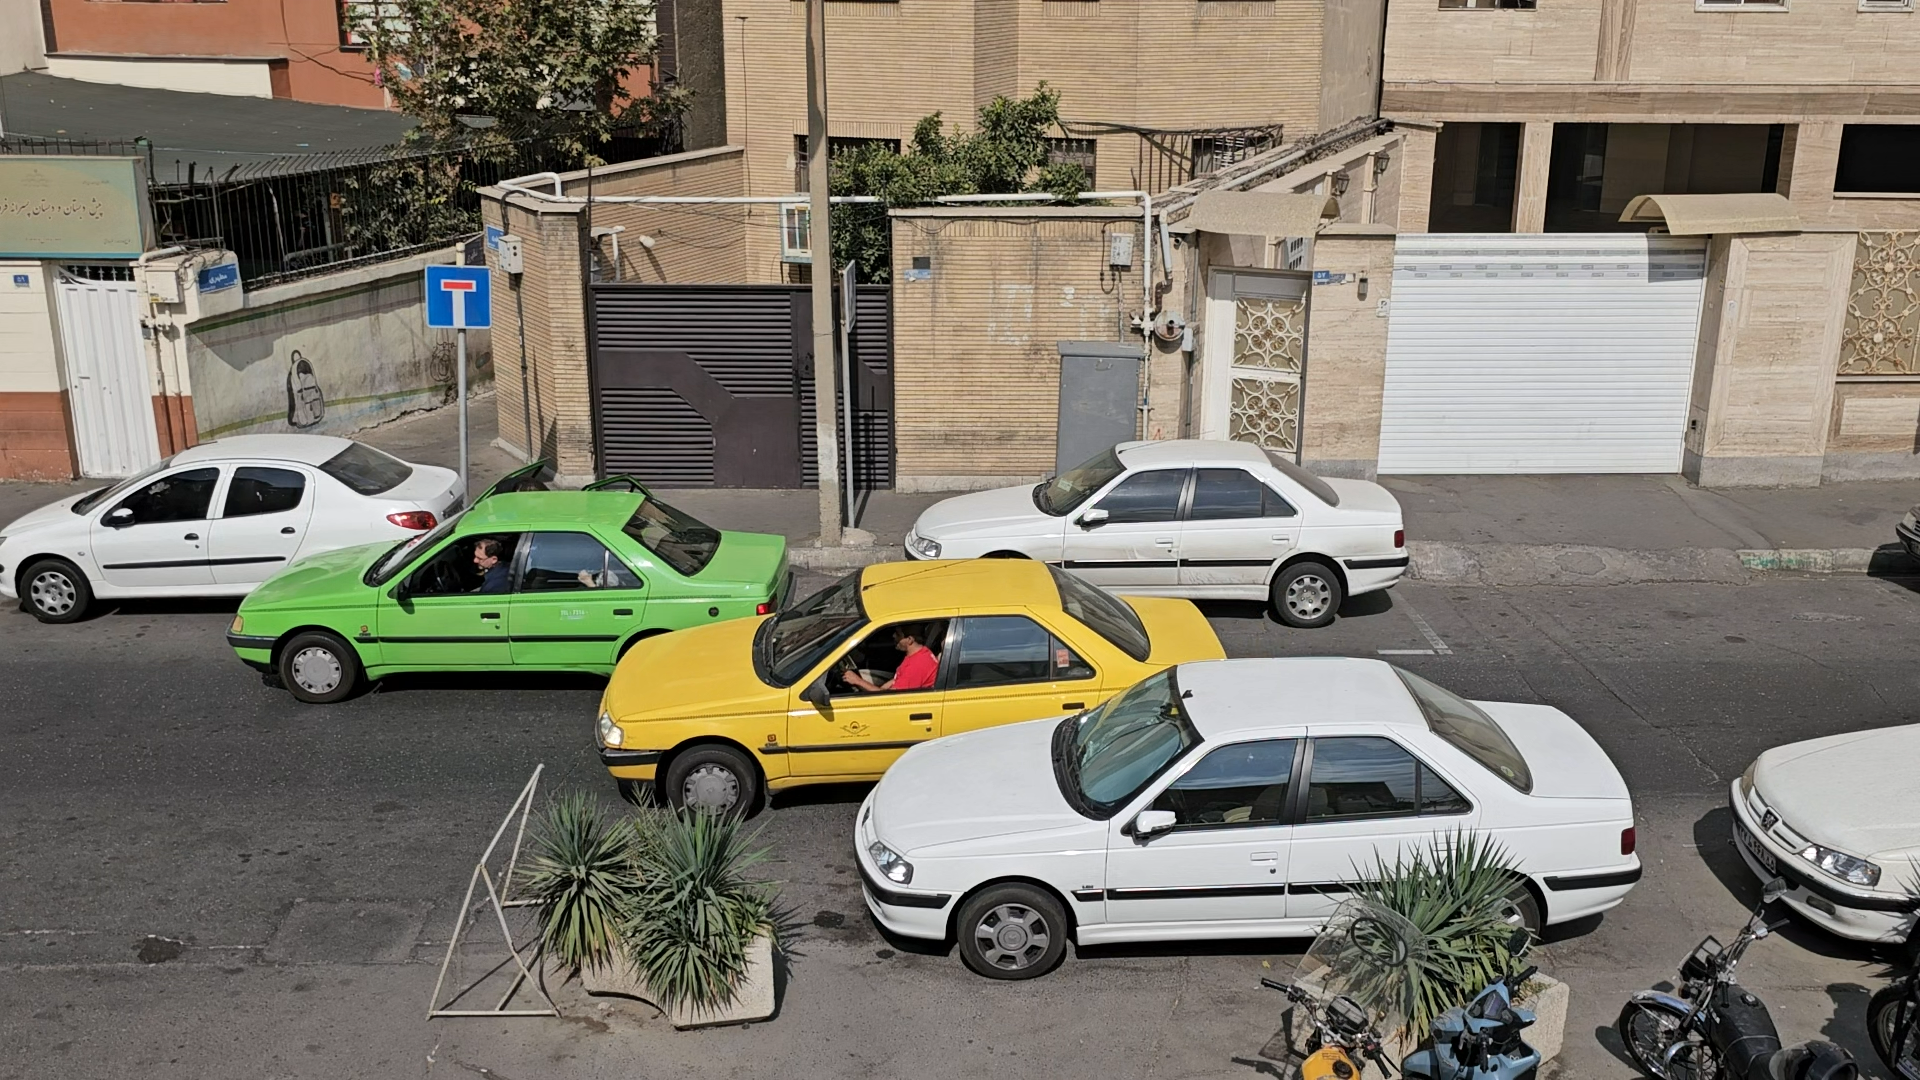
\includegraphics[width=1\linewidth]{figures/Data_Acquisition_Video.png}
    \end{minipage}
    \begin{center}
        \caption{تصاویری از عملیات داده‌برداری}
    \end{center}
    \label{fig:Data_Acquistion}
\end{figure}

\begin{figure}[h!]
    \centering
    \begin{minipage}{0.8\textwidth}
        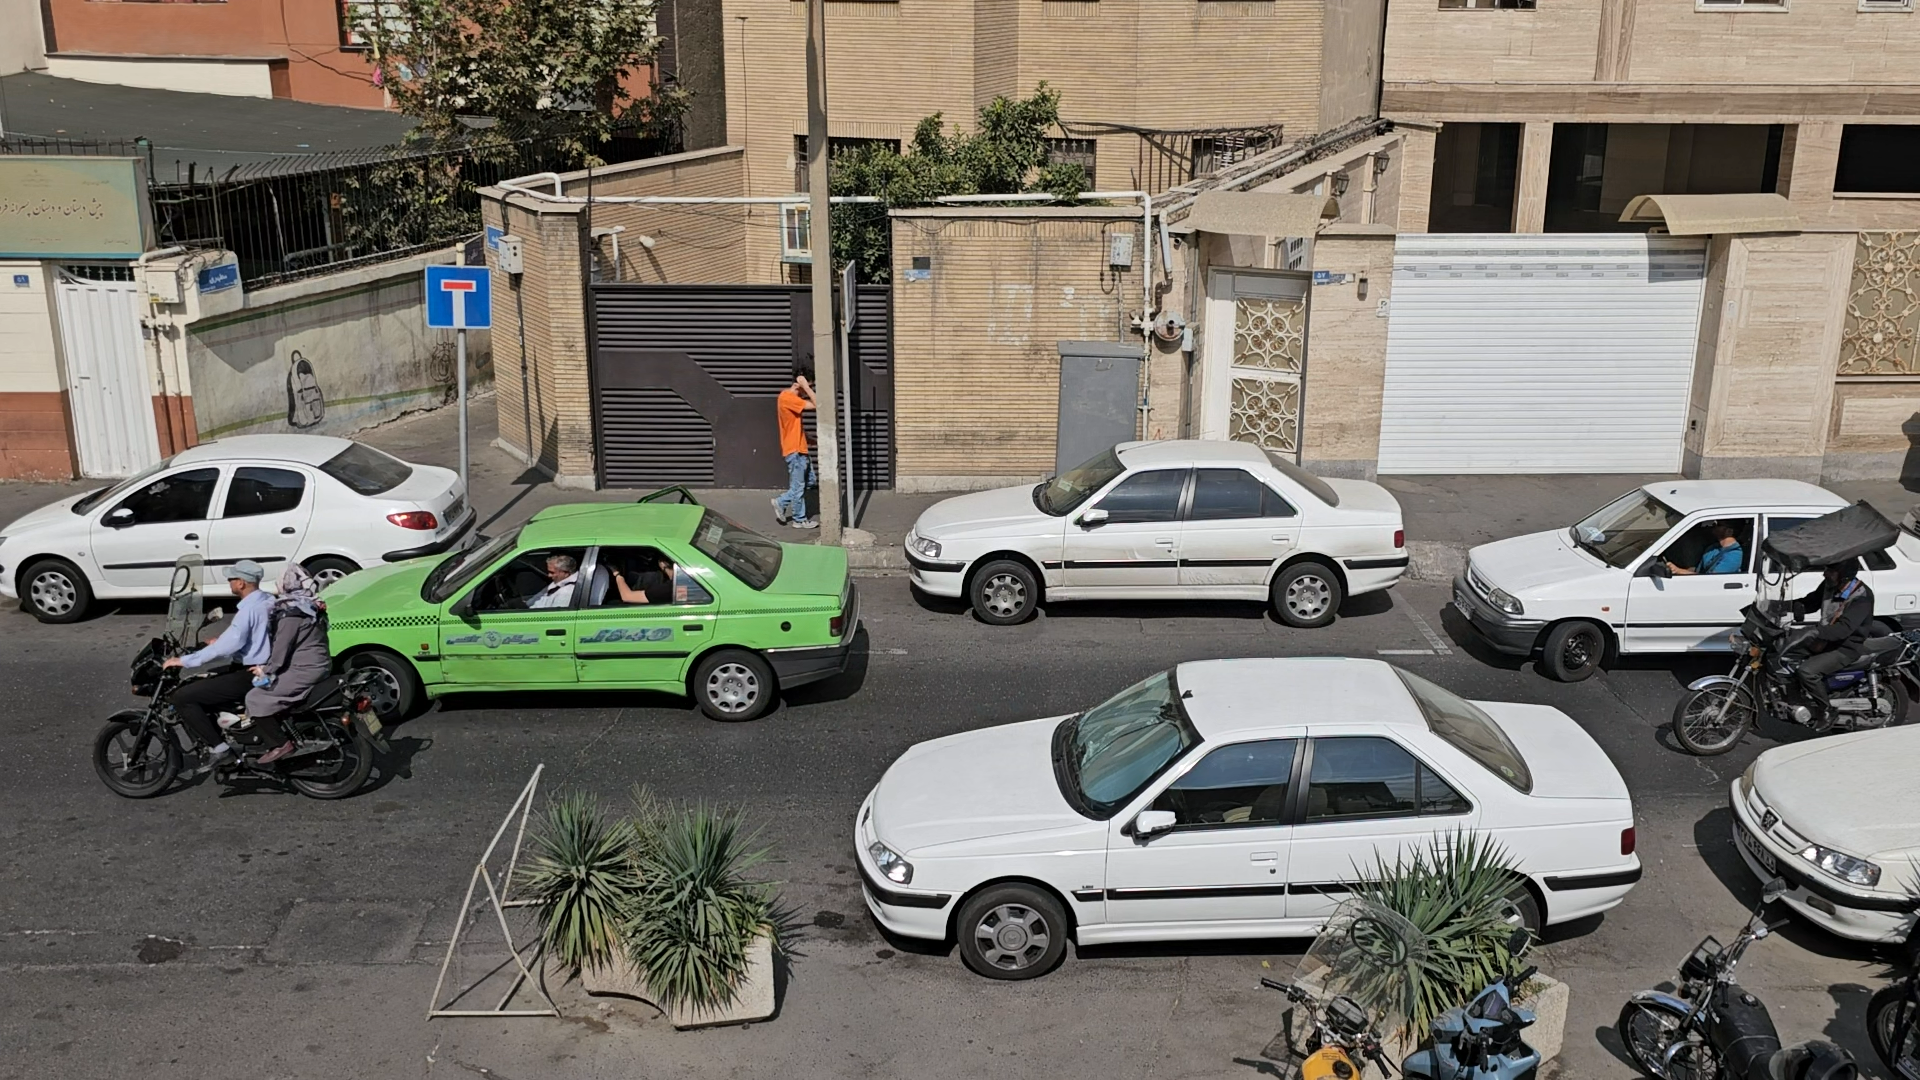
\includegraphics[width=1\linewidth]{figures/Rasht_Lidar_Frame.png}
    \end{minipage}
    \vspace{0.3cm}
    \begin{minipage}{0.8\textwidth}
        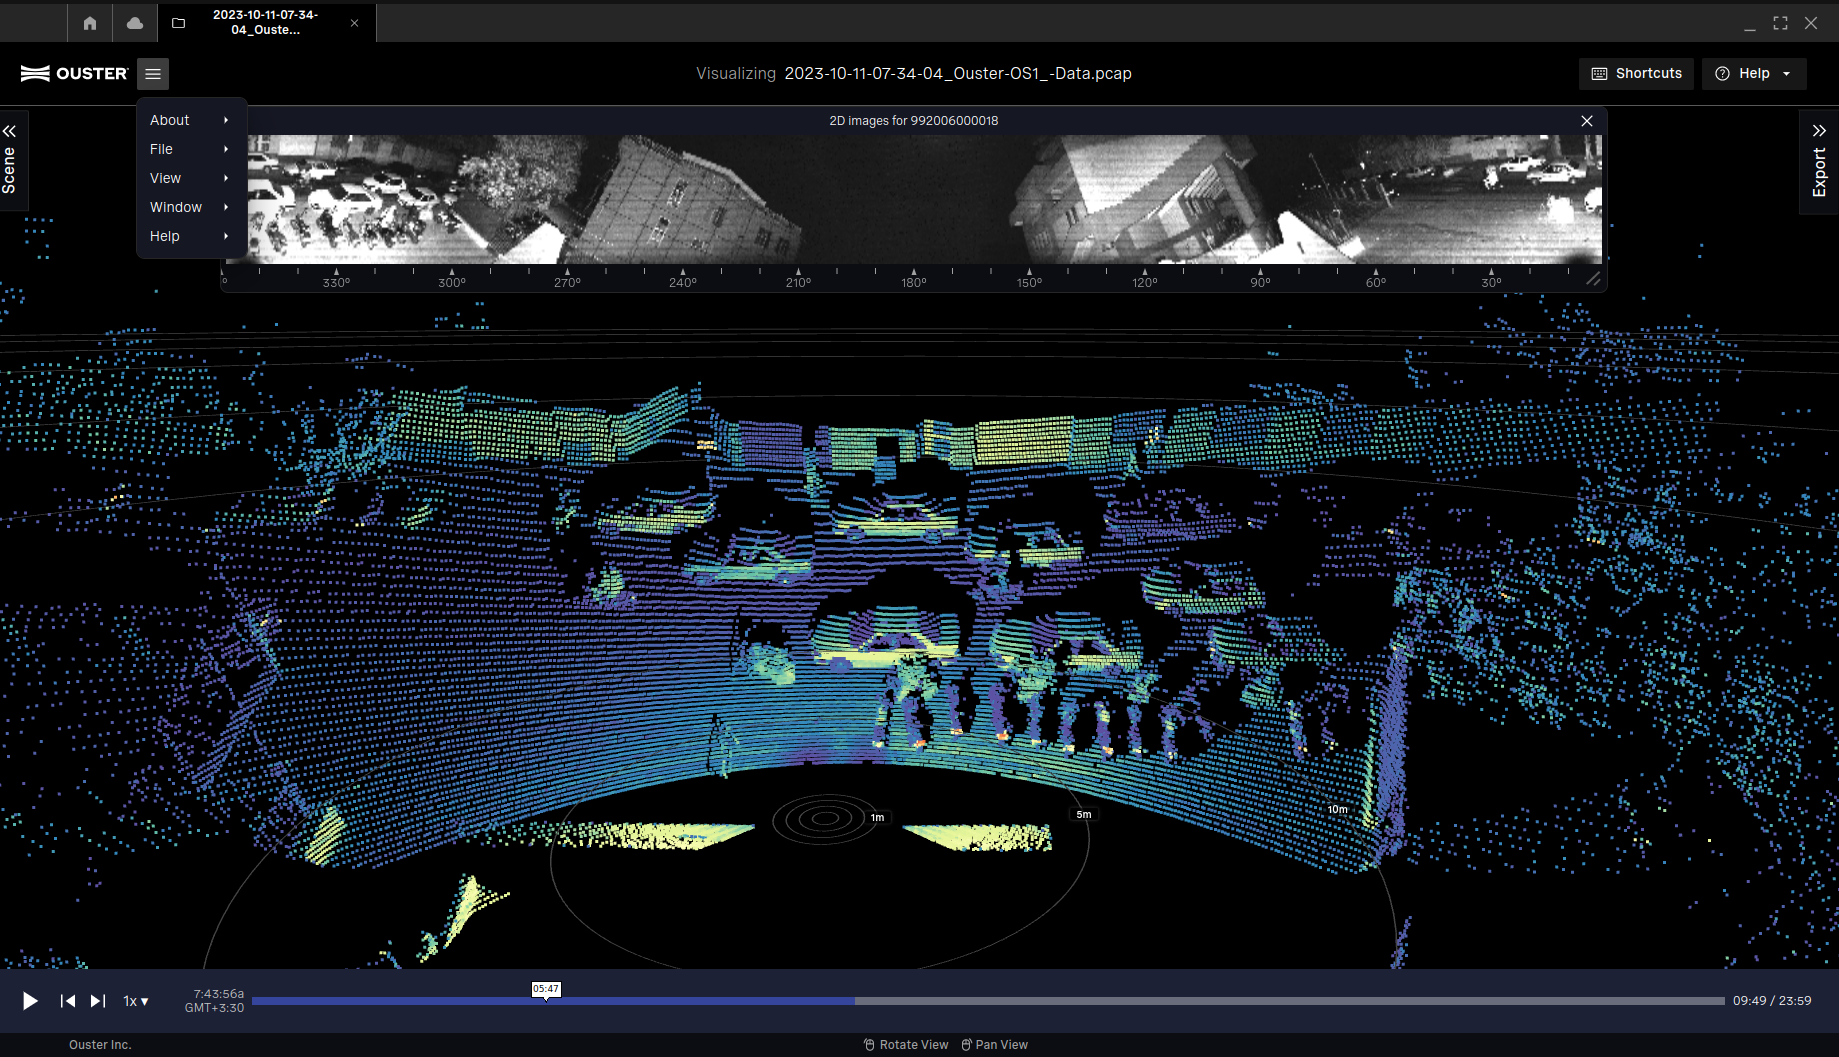
\includegraphics[width=1\linewidth]{figures/Video_Rasht_Frame.png}
    \end{minipage}
    \caption{تصویری از خیابان رشت و ابر نقاط متناظر آن}
    \label{fig:Data_Acquistion_Comparison}
\end{figure}

\begin{figure}[h!]
    \centering
    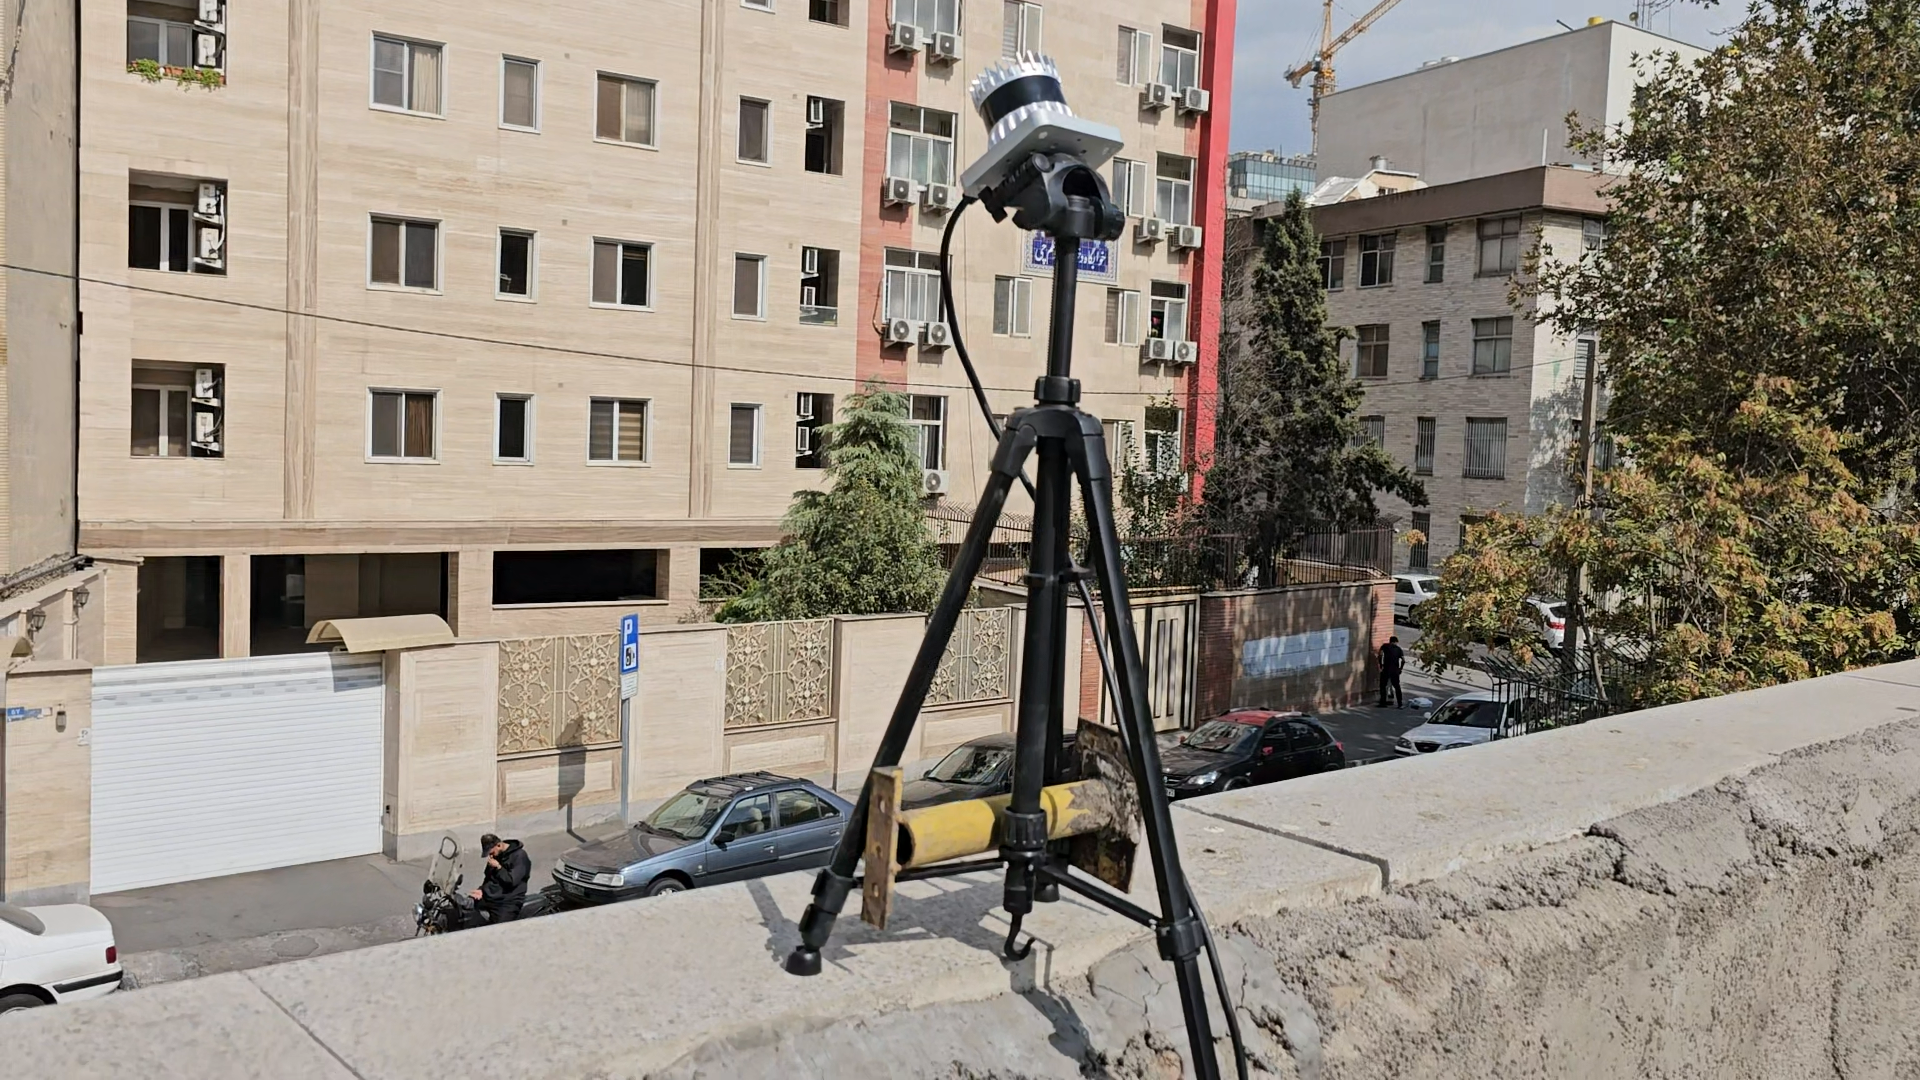
\includegraphics[width=0.75\linewidth]{figures/Lidar_Data_Acquisition2.png}
    \caption{تصویری از لایدار \lr{OS1:64} که بر روی سه‌پایه نصب شده است.}
    \label{fig:Lidar_Data_Acquisition}
\end{figure}

این داده برداری، از ساعت ۹:۳۰ تا ساعت ۱۰:۴۵ ادامه داشت و حسگر لایدار به مدت نیم ساعت داده جمع‌آوری کرد. حجم فایل \lr{.pcap} آن ۷.۱۱ گیگابایت شد.  همانطور که طبق \cref{fig:Lidar_Data_Acquisition} مشاهده می‌کنیم، لایدار نصب شده بر روی سه‌پایه، برای داشتن دید بهتر به خیابان، با سطح افق زاویه دارد. 

\subsection{اعمال مدل هوش‌ مصنوعی به ورودی لایدار}
در بخش قبل، توانستیم با موفقیت یک ضبط لایدار نیم ساعته از خیابان رشت ضبط کنیم. این ضبط در فرمت \lr{"*.pcap"} ذخیره شده است، پس می‌توانیم آن را به خورد تبدیل‌کننده \lr{pcap\_to\_pointcloud2\_py} بدهیم. \begin{figure}[h]
    \centering
    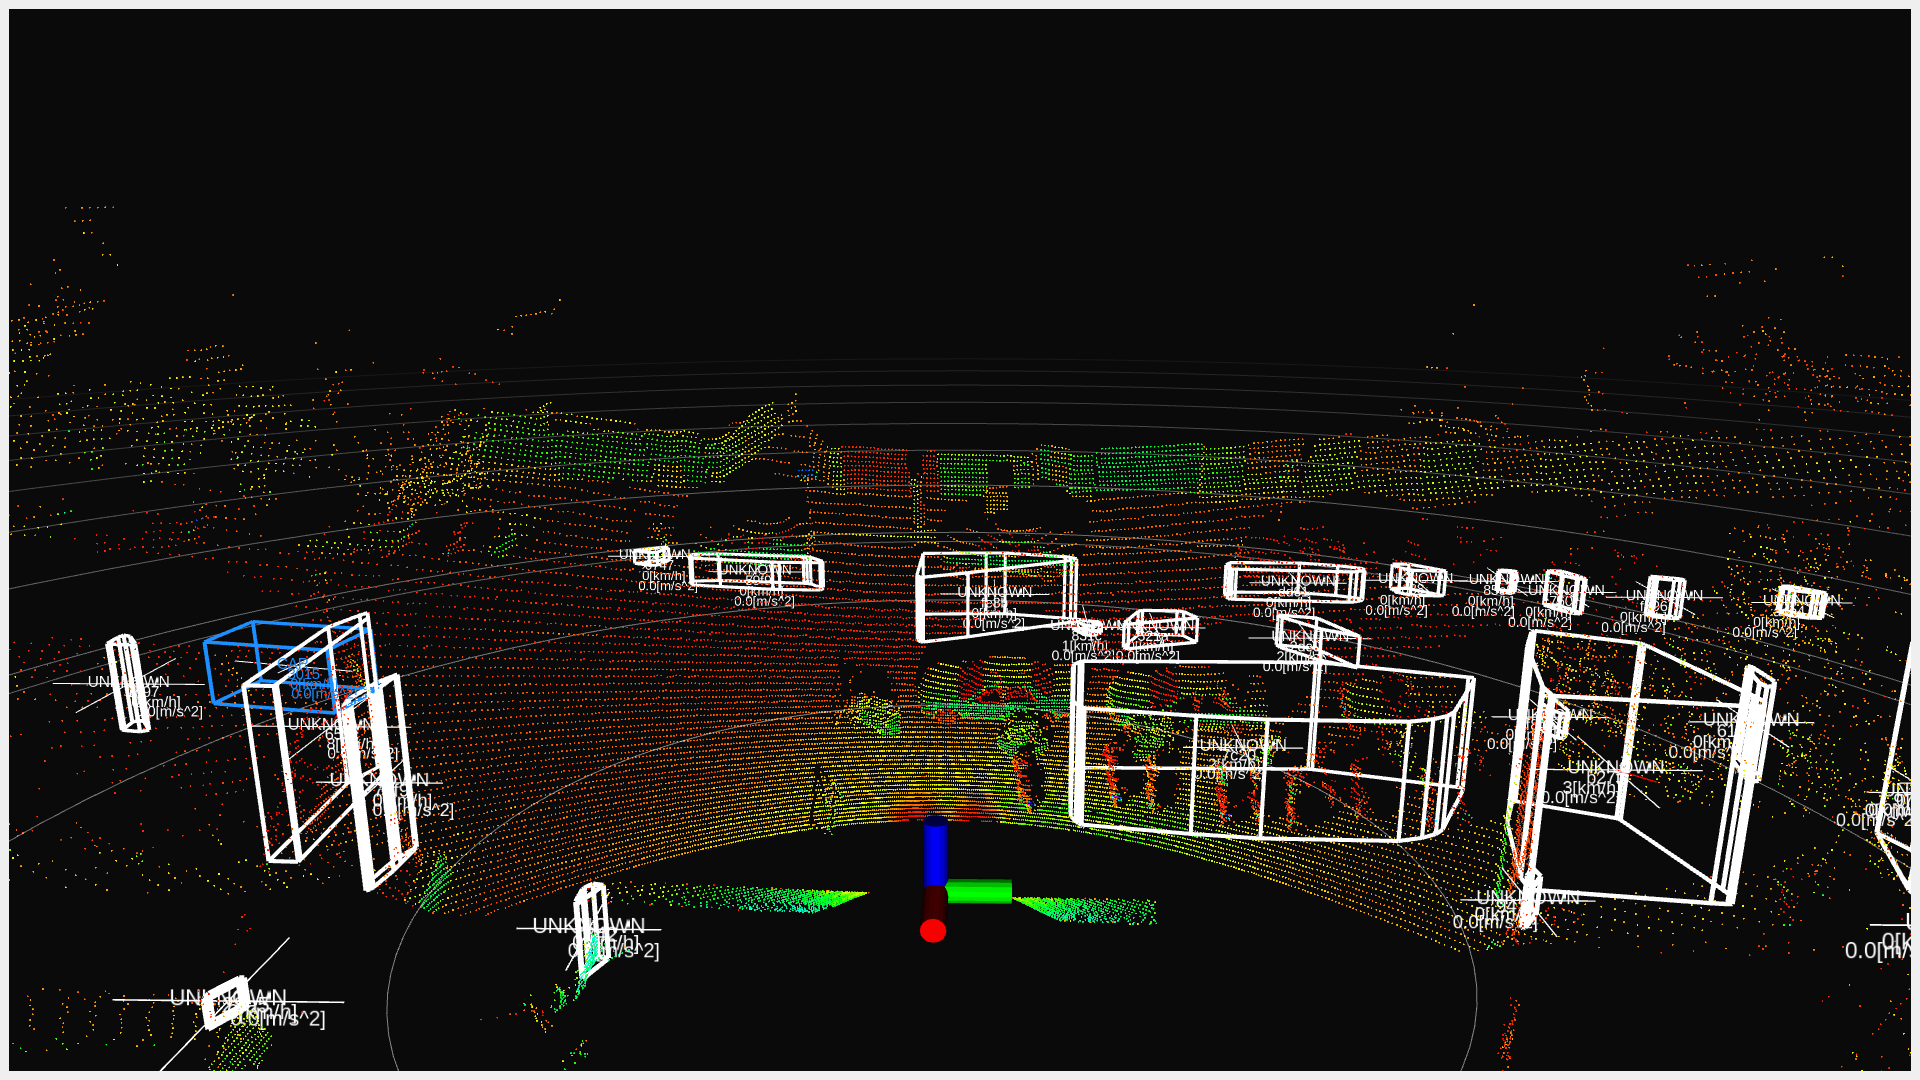
\includegraphics[width=0.9\linewidth]{figures/Rasht_Uncalibrated_Detection_Attempt.png}
    \caption{اقدام ناموفق تشخیص بر روی ابر‌ نقاط خیابان رشت}
    \label{fig:Rasht_Uncalibrated_Detection_Attempt}
\end{figure}
همچنین می‌توانیم این داده تبدیل‌ شده به \lr{PointCloud2} را برای مبحث ورودی مولفه ادراک \lr{Autoware}، منتشر کنیم و عملیات تشخیص بلادرنگ بر روی آن انجام شود. \cref{fig:Rasht_Uncalibrated_Detection_Attempt} نشان می‌دهد که تشخیص بر روی ابر نقاط رشت، به درستی کار نمی‌کند. دلیل این اتفاق با توجه کردن به همین شکل و \cref{fig:Lidar_Data_Acquisition} قابل فهم است. در بخش قبلی ذکر کردیم که لایدار، با سطح افقی، زاویه دارد. پس ابر‌ نقاطی که ضبط می‌کند نیز نسبت به افق زاویه خواهند داشت. به عبارت دیگر، ابر نقاط این لایدار کالیبره\LTRfootnote{\lr{Calibration}} نشده‌اند.
\begin{figure}
    \centering
    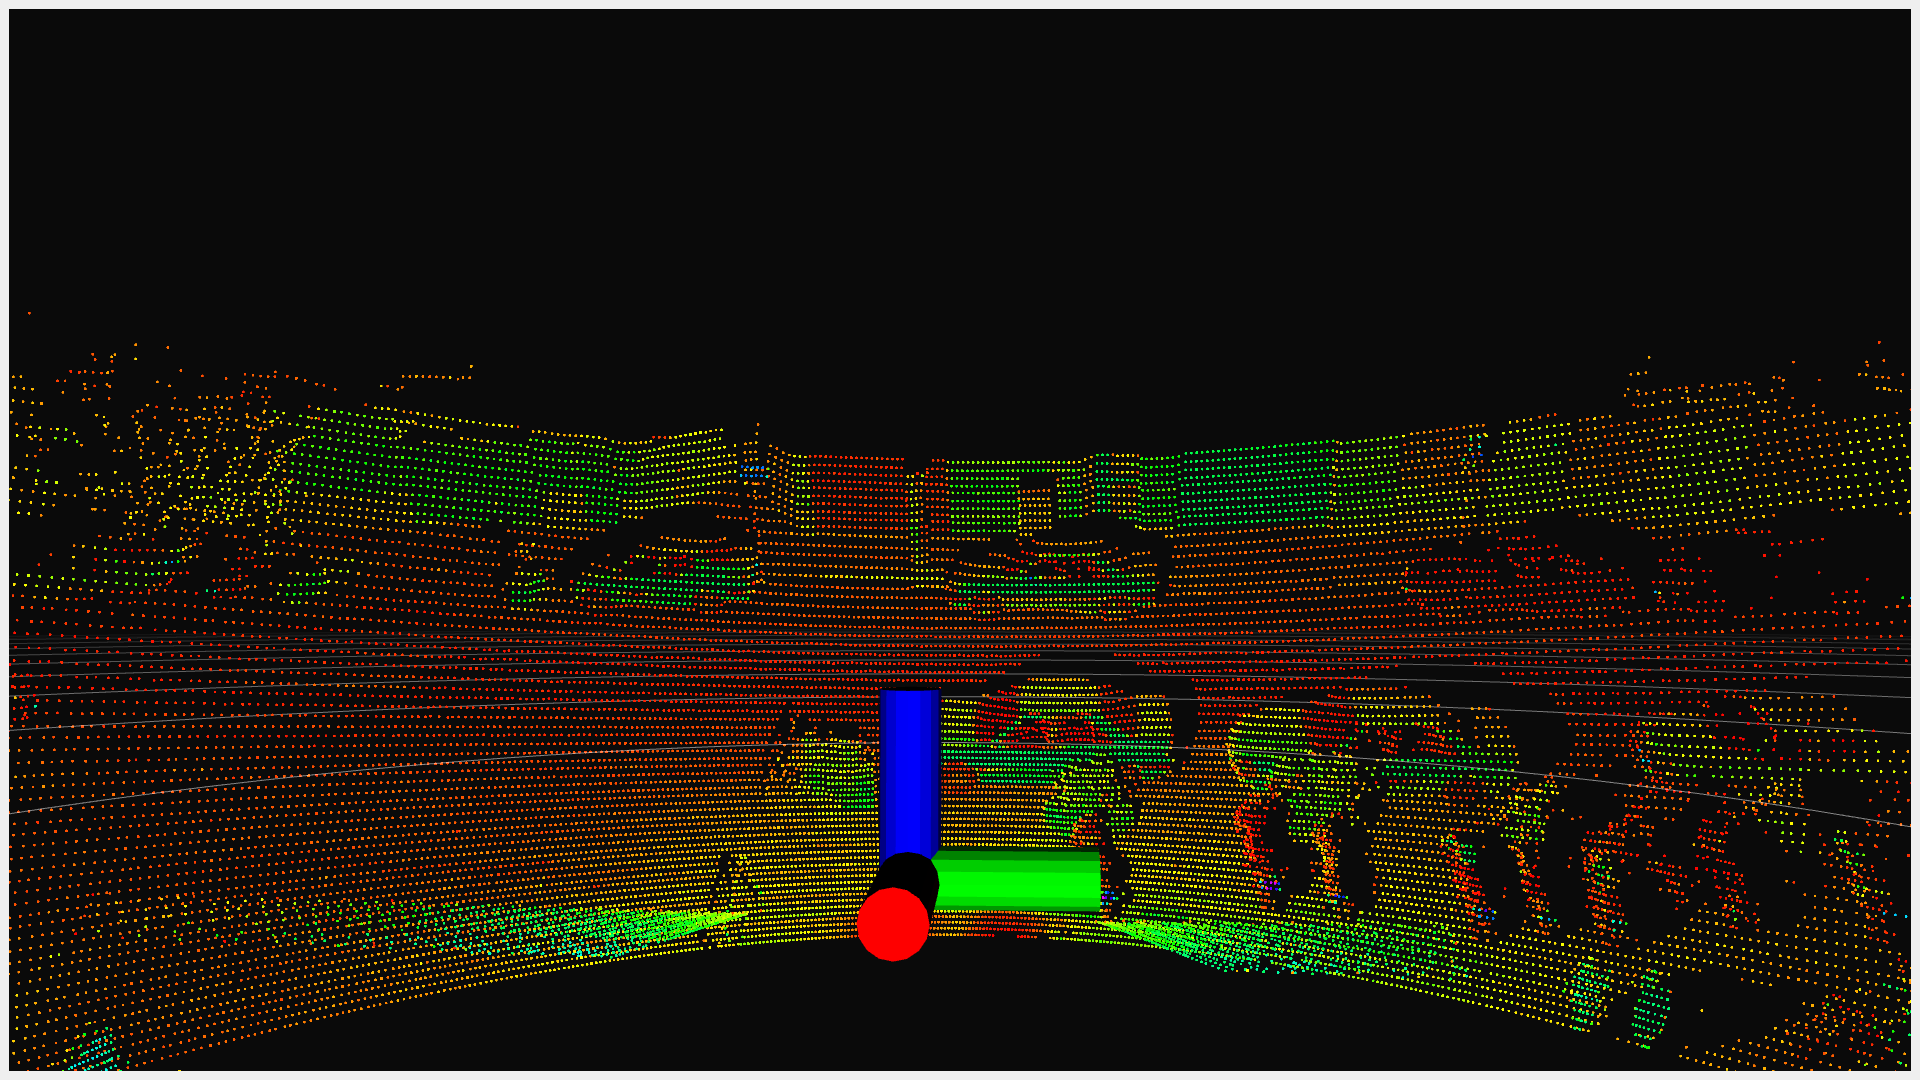
\includegraphics[width=1\linewidth]{figures/Rasht_Uncalibrated_Pointcloud.png}
    \caption{نمای نزدیک از کالیبره نبودن ابر نقاط خیابان رشت.}
    \label{fig:Rasht_Uncalibrated_Pointcoud}
\end{figure}
\cref{fig:Rasht_Uncalibrated_Pointcoud}، این مشکل را به وضوح نمایان می‌کند. برای حل این مشکل، نیاز است تا زاویه لایدار را نسبت به سطح افق بدست بیاوریم. از آنجایی که سه‌‌پایه استفاده شده در داده‌برداری، دست نخورده بود؛ توانستیم زاویه لایدار را با افق بدست بیاوریم. زاویه لایدار با سطح افق، مقدار ۵۱.۳۱ درجه یا ۵۵.۱ رادیان در محور $Y$ است. همچنین با کمی دقت در ‌\cref{fig:Rasht_Uncalibrated_Detection_Attempt}، متوجه می‌شویم که محور مختصات لایدار برعکس است، یعنی پشت لایدار به سمت خیابان رشت بوده است. پس لازم است تا محور مختصات $XY$ را ۱۸۰ درجه حول محور $Z$ بچرخانیم. در نهایت نیز به نتیجه رسیده شد که ارتفاع لایدار نسبت به سطح زمین، ۶ متر است. پس بایستی محور مختصات لایدار را ۶ متر به سمت بالا حرکت دهیم تا سطح زمین خیابان رشت، هم سطح نقطه $(0,0,0)$ یا همان محور مختصات دنیای \lr{ROS2} شود. فرمول ماتریس دوران\LTRfootnote{\lr{Rotation Matrix}} در فضای سه‌بعدی به شکل زیر است:
\begin{equation}
    \mathbf{R} = \mathbf{R_z(\psi)}\mathbf{R_y(\theta)}\mathbf{R_x(\phi)} = \begin{bmatrix}
        c_{\psi}c_{\theta} & c_{\psi}s_{\theta}s_{\phi} - s_{\psi}c_{\phi} & c_{\psi}s_{\theta}c_{\phi} + s_{\psi}s_{\phi} \\
        s_{\psi}s_{\theta} & s_{\psi}s_{\theta}s_{\phi} + c_{\psi}c_{\phi} & s_{\psi}s_{\theta}s_{\phi} + c_{\psi}c_{\phi} \\
        -s_{\theta} & c_{\theta}s_{\phi} & s_{\theta}c_{\phi}\\
    \end{bmatrix}
\end{equation}
و بردار انتقال به شکل زیر است:
\begin{equation}
    \mathbf{T} = 
    \begin{bmatrix}
        t_x \\
        t_y \\
        t_z \\
    \end{bmatrix}
\end{equation}
با عدد گذاری در روابط فوق، خواهیم داشت:
\begin{align*}
    \mathbf{R} &= 
    \begin{bmatrix}
        0.8525245 & 0 & -0.5226873 \\
        0 & 1 & 0 \\
        0.526873 & 0 & 0.8525245 \\
    \end{bmatrix}
    &
    \mathbf{T} &= 
    \begin{bmatrix}
        0 \\
        0 \\
        6 \\
    \end{bmatrix}
\end{align*}
و به ازای هر نقطه $P$ داخل ابر‌نقطه خواهیم داشت:
\begin{align}
    \mathbf{P_{new}} = \mathbf{R}\mathbf{P} + \mathbf{T}
\end{align}
بهترین جا برای اعمال این تبدیل‌ها، در داخل کد \lr{pcap\_to\_pointcloud\_py} است، زیرا در هر فریم از ضبط لایدار، مختصات $(X,Y,Z)$ نقطه‌ها بدست می‌آید. پس می‌توانیم ماتریس تبدیل و دوران را بر روی این مختصات‌ها اعمال کنیم. حال، باری دیگر ابر نقاط خیابان رشت را به خورد تشخیص‌دهنده می‌دهیم، اما با این تفاوت که این دفعه ابر نقاط کالیبره شده‌اند.

\begin{figure}[h!]
    \centering
    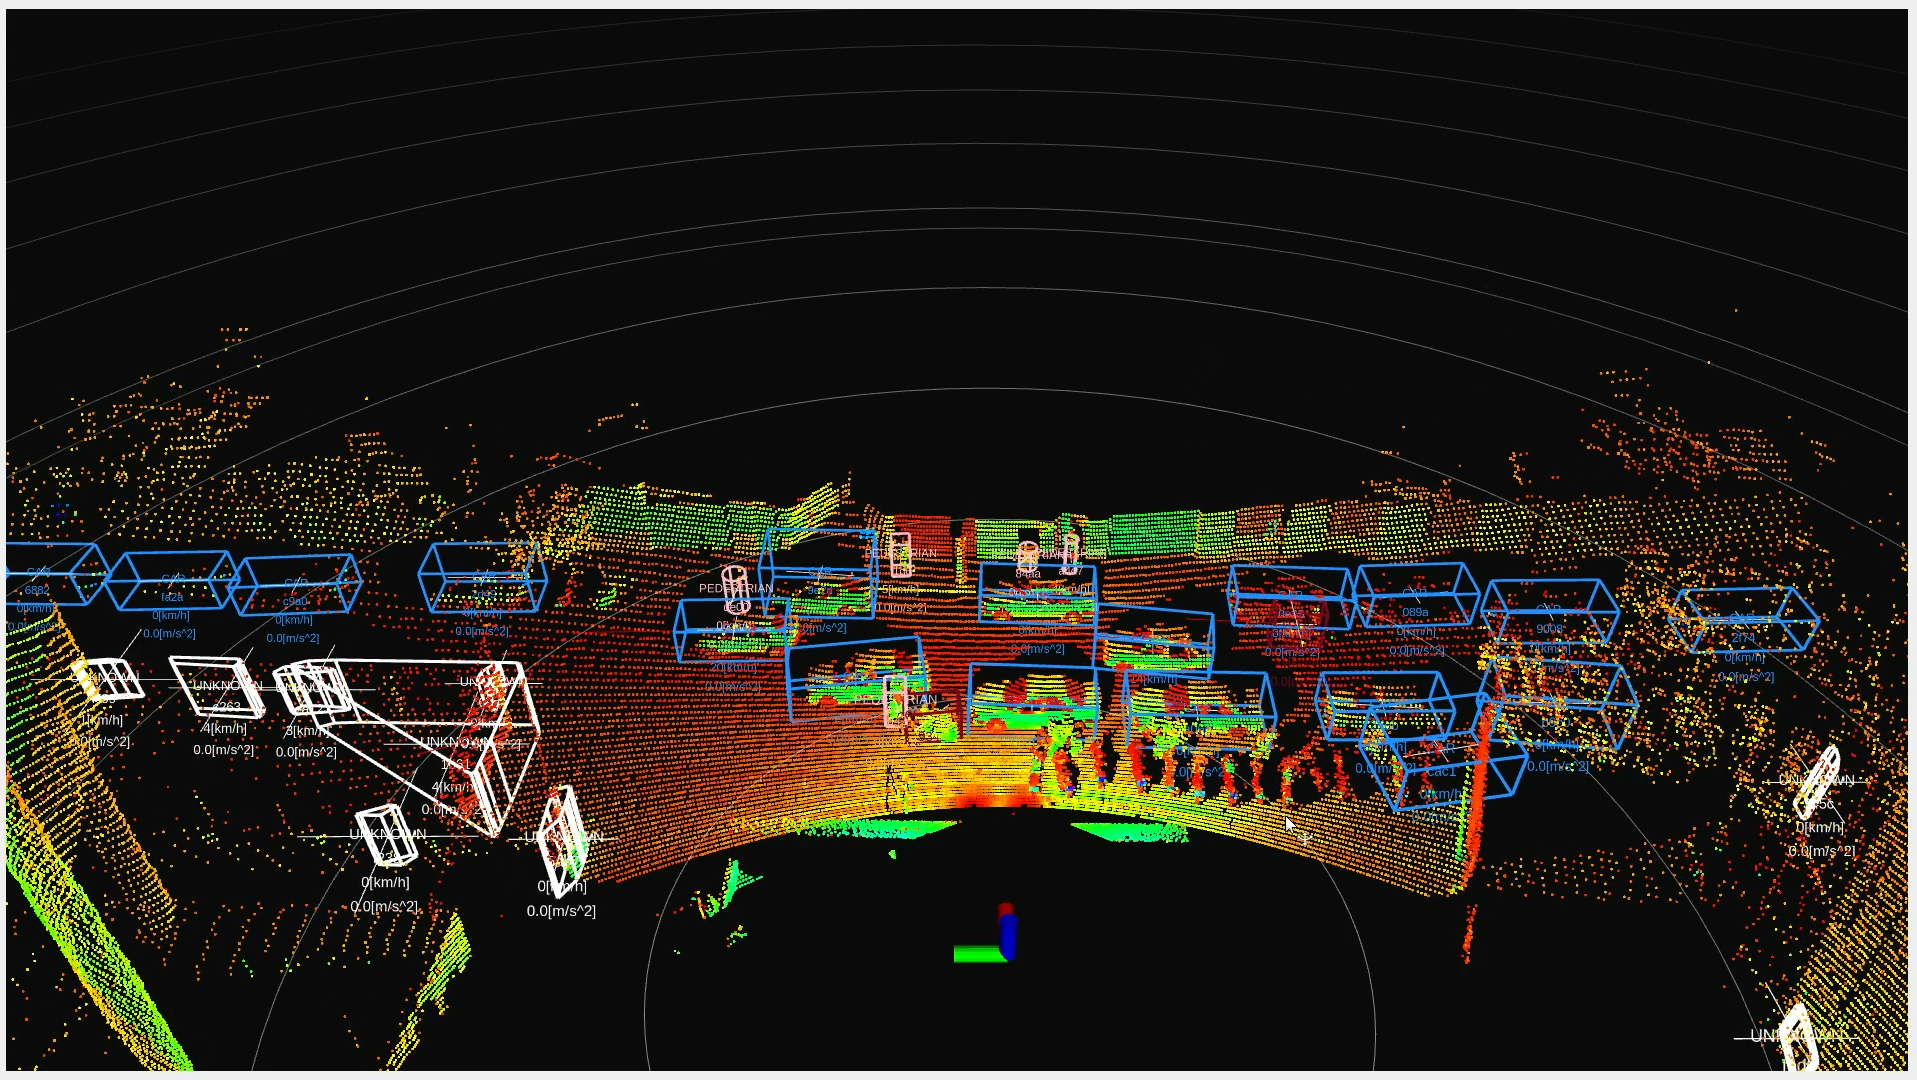
\includegraphics[width=1\linewidth]{figures/Rasht_Calibrated_3D_Detection.png}
    \caption{تشخیص موفق اجسام با ورودی ابر نقاط کالیبره شده}
    \label{fig:Rasht_Calibrated_3D_Detection}
\end{figure}

همانطور که از \cref{fig:Rasht_Calibrated_3D_Detection} نمایان است، تشخیص اجسام با موفقیت انجام شده است. حال تصویری از دوربین را در مقابل ابر نقاط متناظر آن قرار می‌دهیم:

\begin{figure}[h!]
    \centering
    \begin{minipage}{1\textwidth}
        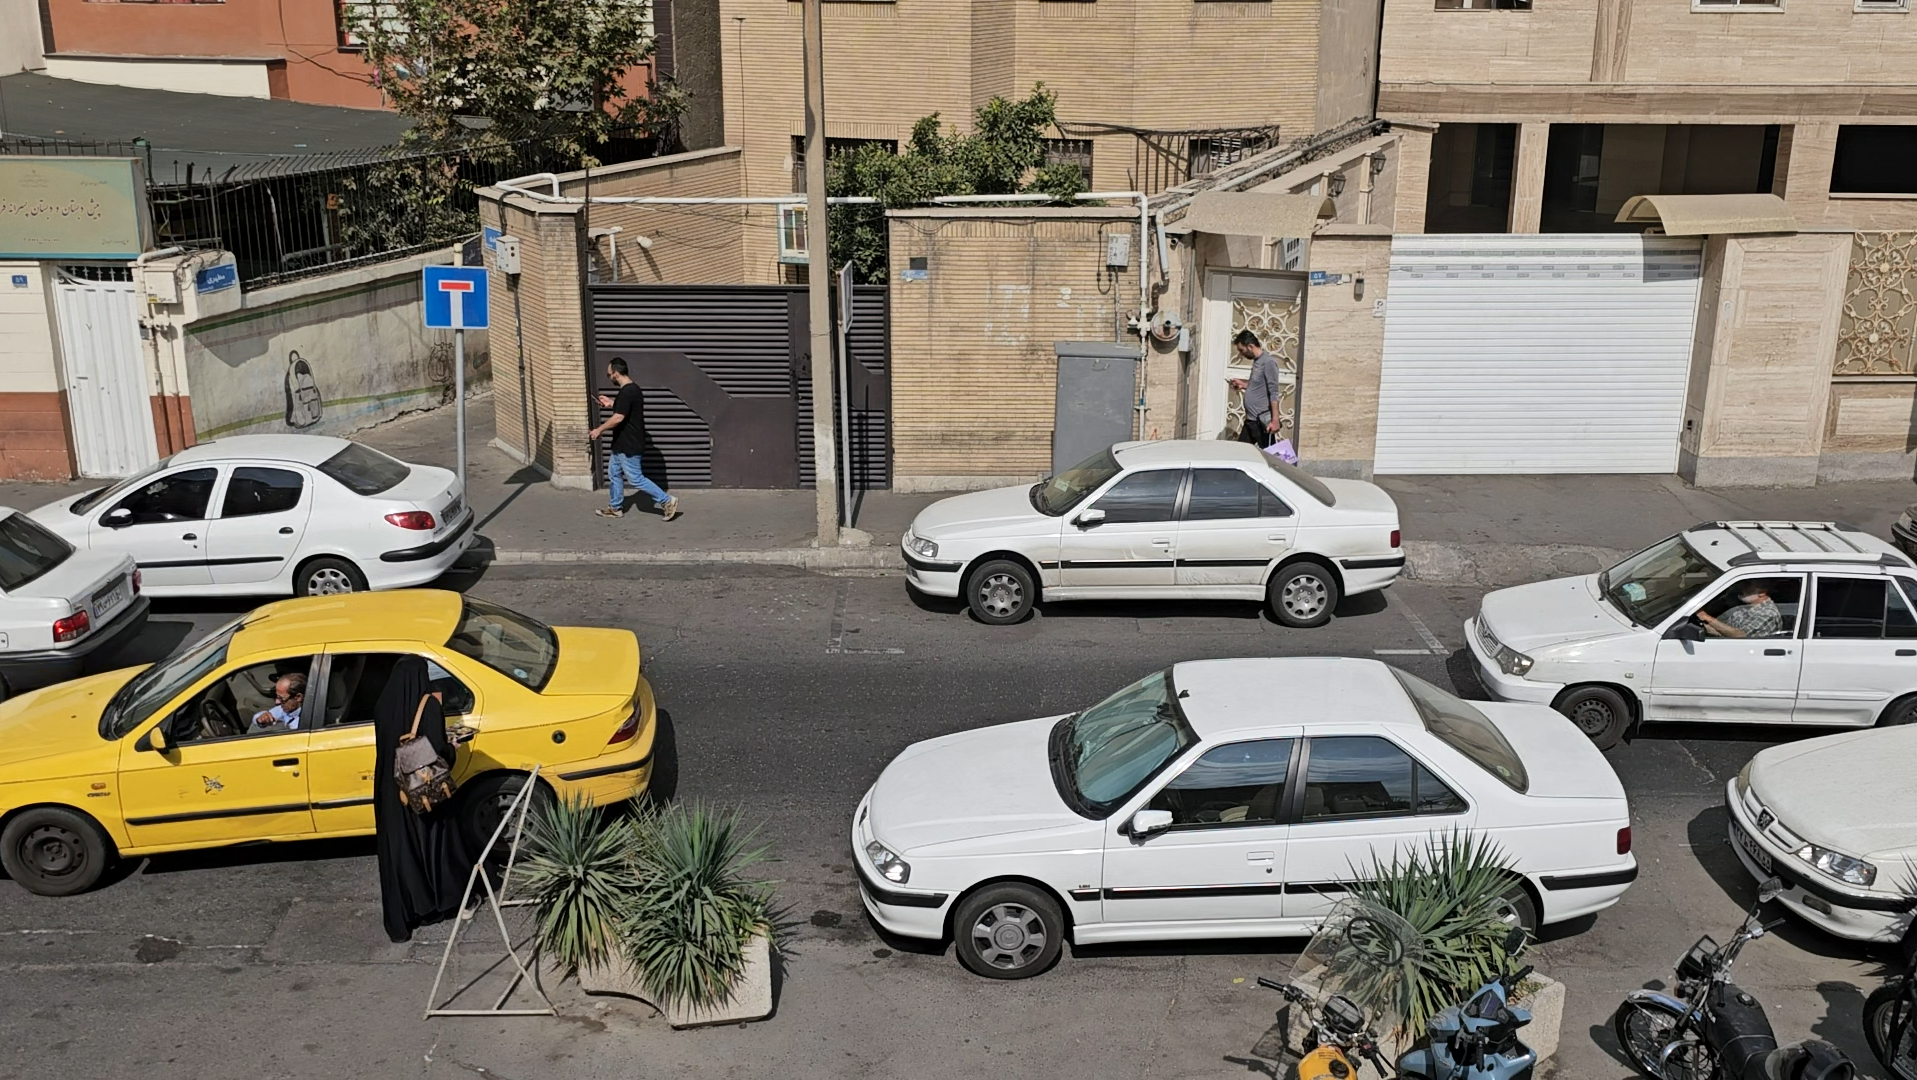
\includegraphics[width=1\linewidth]{figures/Rasht_Video_Frame_3D_Detection.png}
    \end{minipage}
    \vspace{0.3cm}
    \begin{minipage}{1\textwidth}
        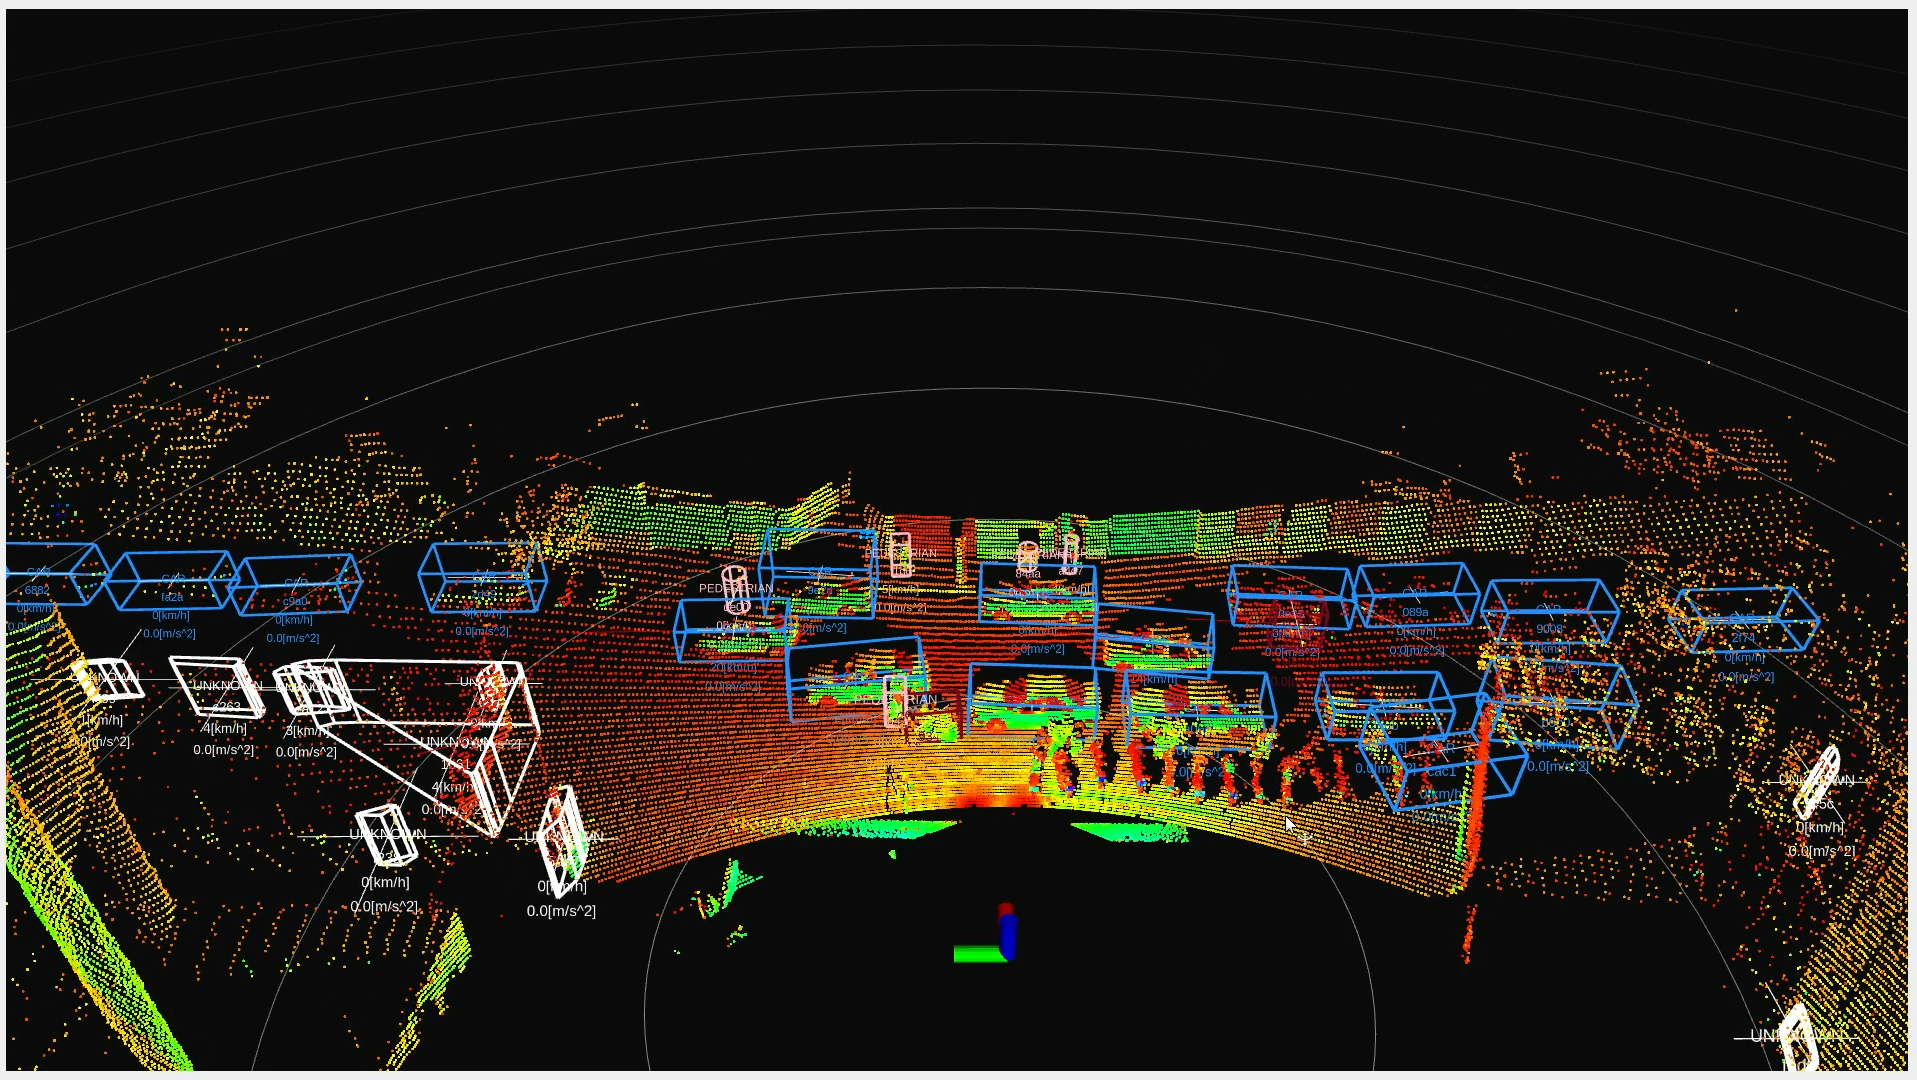
\includegraphics[width=1\linewidth]{figures/Rasht_Calibrated_3D_Detection.png}
    \end{minipage}
    \caption{تصویری از خیابان رشت و ابر نقاط پردازش‌ شده‌ی متناظر آن}
    \label{fig:3D_Detection_Comparison}
\end{figure}

\section{طراحی مدل سه‌بعدی منطقه دانشگاه صنعتی امیرکبیر}

آخرین مرحله باقی‌ مانده، طراحی فضای پردیس امیرکبیر است. در فصل دوم، مقاله‌ای را معرفی کردیم که در سال ۲۰۲۲ نوشته شده است و در مورد روش‌های بهینه مدل‌سازی سه‌بعدی دوقلوهای دیجیتال صحبت کرده است \cite{azfar2022efficient}. باری دیگر شکل روند طی شده برای مدل‌سازی سه‌بعدی این مقاله را مرور می‌کنیم:

\begin{figure}[h!]
	\centering
	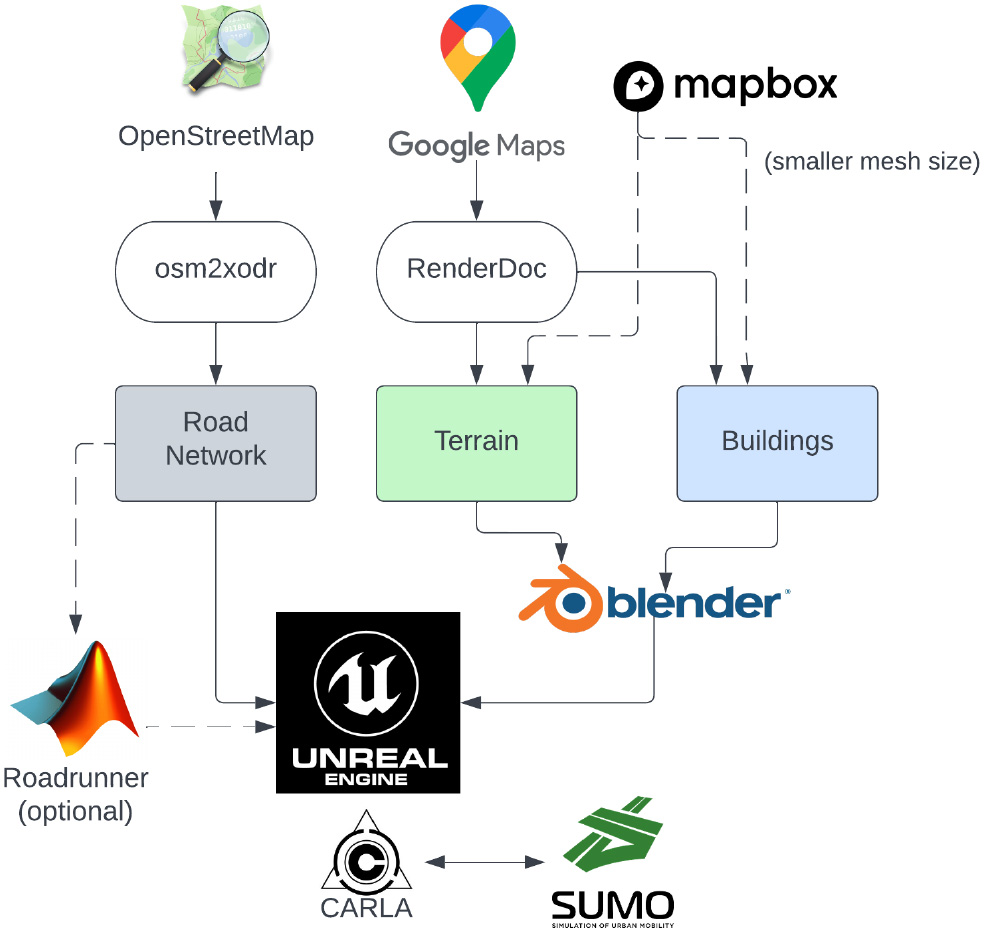
\includegraphics[width=0.75\linewidth]{figures/Digital_Twin_Procedure.png}
	\caption{   روش پیشنهاد شده برای ایجاد دوقلوی دیجیتال یک منطقه \cite{azfar2022efficient}}
	\label{fig:dt_procedure_1}
\end{figure}

این مقاله با استفاده از داده‌های ابزار \lr{OpenStreetMap}، که در آن خیابان‌ها، ساختمان‌ها و انواع داده‌های دیگر مرتبط با نقشه بُرداری را در خود دارد. از فصل سوم نیز به یاد داریم که افزونه‌ای در ابزار طراحی مدل‌های سه‌بعدی \lr{Blender} وجود دارد، که \lr{Blosm} نام دارد. این افزونه با استفاده از داده‌های \lr{"*.os"} گرفته شده از ابزار \lr{OpenStreetMap}، مدل سه‌بعدی یک منطقه را تنها با چندین کلیک دکمه انجام می‌دهد! این افزونه، از ابزاری به نام \lr{MapBox}\LTRfootnote{\url{https://www.mapbox.com/}} استفاده می‌کند که تمامی اطلاعات مهم از یک نقشه را دارد. این ابزار، در بسیاری از برنامه‌های مسیریاب، نقشه سه‌بعدی و ناوبری استفاده می‌شود. برای اینکه افزونه \lr{Blosm} بتواند اطلاعات نقشه سه‌بعدی یک منطقه را با استفاده از واسط برنامه‌نویسی کاربری\LTRfootnote{\lr{Application Programming Interface (API)}} \lr{MapBox Streets} بدست بیاورد، نیاز به یک کلید \lr{API} است. برای دستیابی به این کلید، نیاز است که در تارنمای این ابزار ثبت‌نام کرد. اما برای آنکه اثبات شود که کاربرهای در حال ثبت‌نام، ربات نیستند؛ این ابزار نیاز به مشخصات کارت اعتباری\LTRfootnote{\lr{Credit Card}} بین‌المللی دارد.
\begin{figure}[h!]
    \centering
    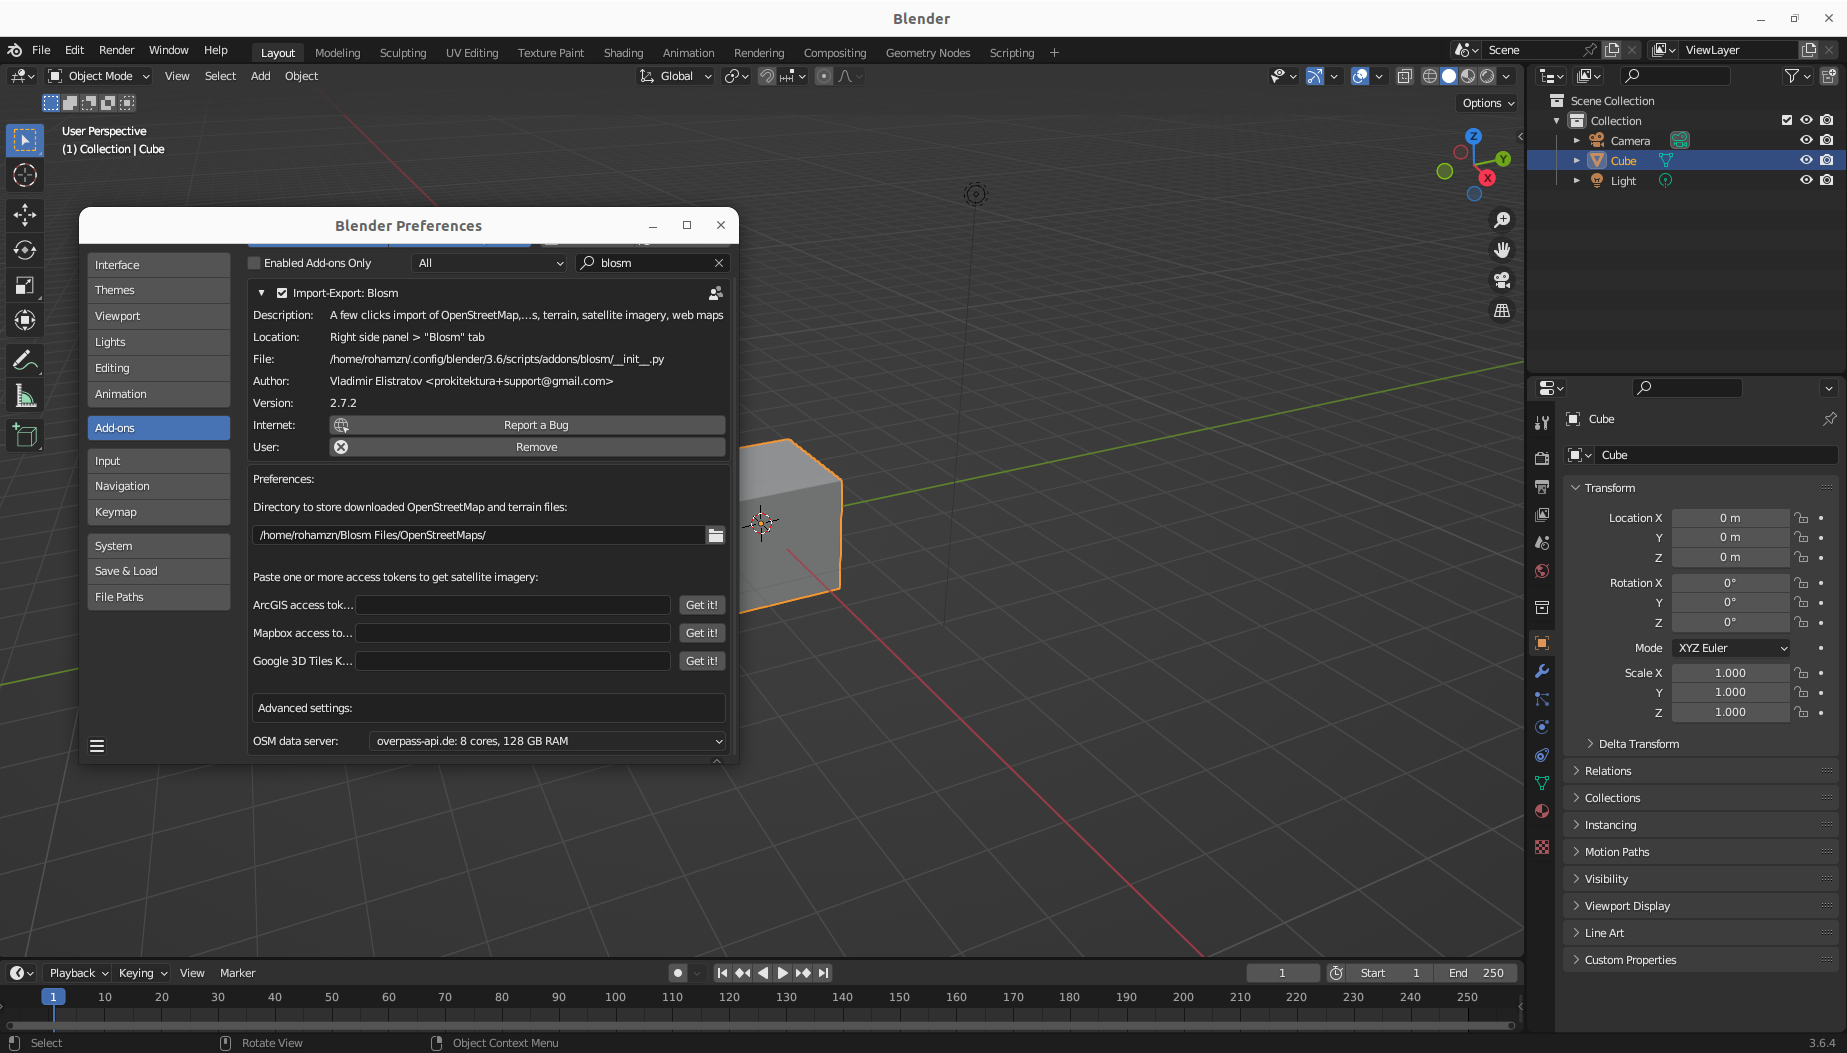
\includegraphics[width=0.9\linewidth]{figures/Blender_Blosm.png}
    \caption{نمایی از افزونه \lr{Blosm} در ابزار مدل‌سازی سه‌بعدی \lr{Blender}}
    \label{fig:Blender_Blosm}
\end{figure}
طبق \cref{fig:Blender_Blosm}، مشاهده می‌کنیم که این افزونه یک کلید \lr{API} از ابزار \lr{MapBox} می‌خواهد. با پیش‌روی طبق مقاله ذکر شده، منطقه امیرکبیر را در این افزونه انتخاب می‌کنیم تا از آن یک مدل سه‌بعدی بسازد. 
\begin{figure}[h!]
    \centering
    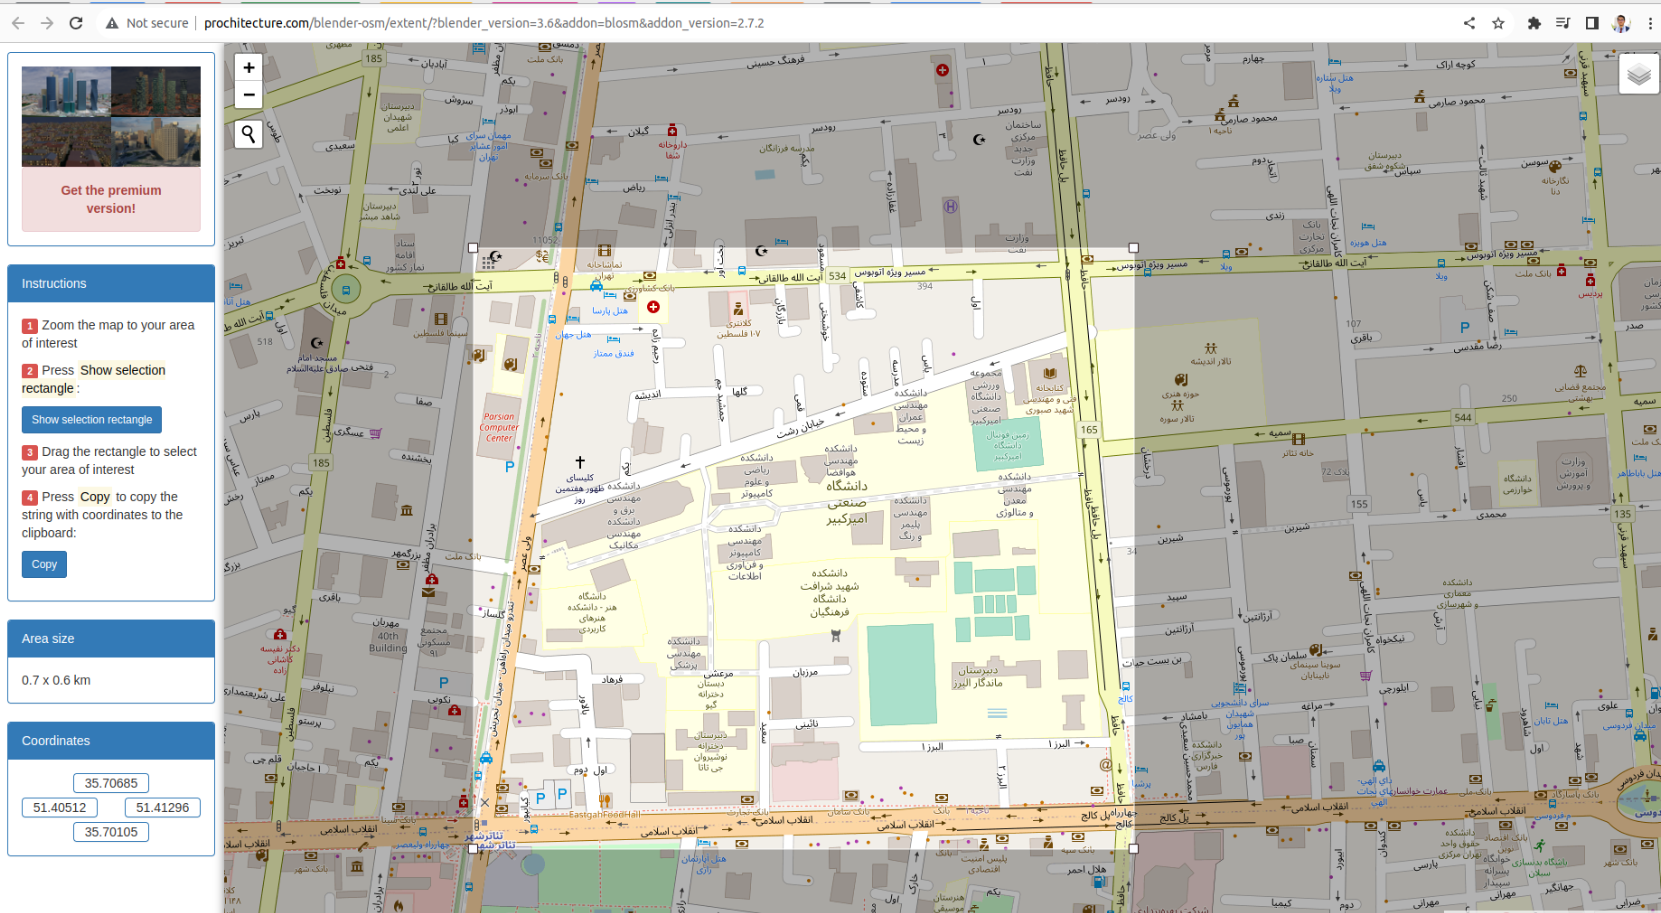
\includegraphics[width=1\linewidth]{figures/Blosm_OSM.png}
    \caption{منظقه انتخاب شده در افزونه \lr{Blosm}}
    \label{fig:Blosm_OSM}
\end{figure}
پس از انتخاب محل، دکمه ساختن مدل را می‌زنیم و پس از کمی صبر کردن، مدل سه‌بعدی زیر را مشاهده می‌کنیم. 
\begin{figure}[h!]
    \centering
    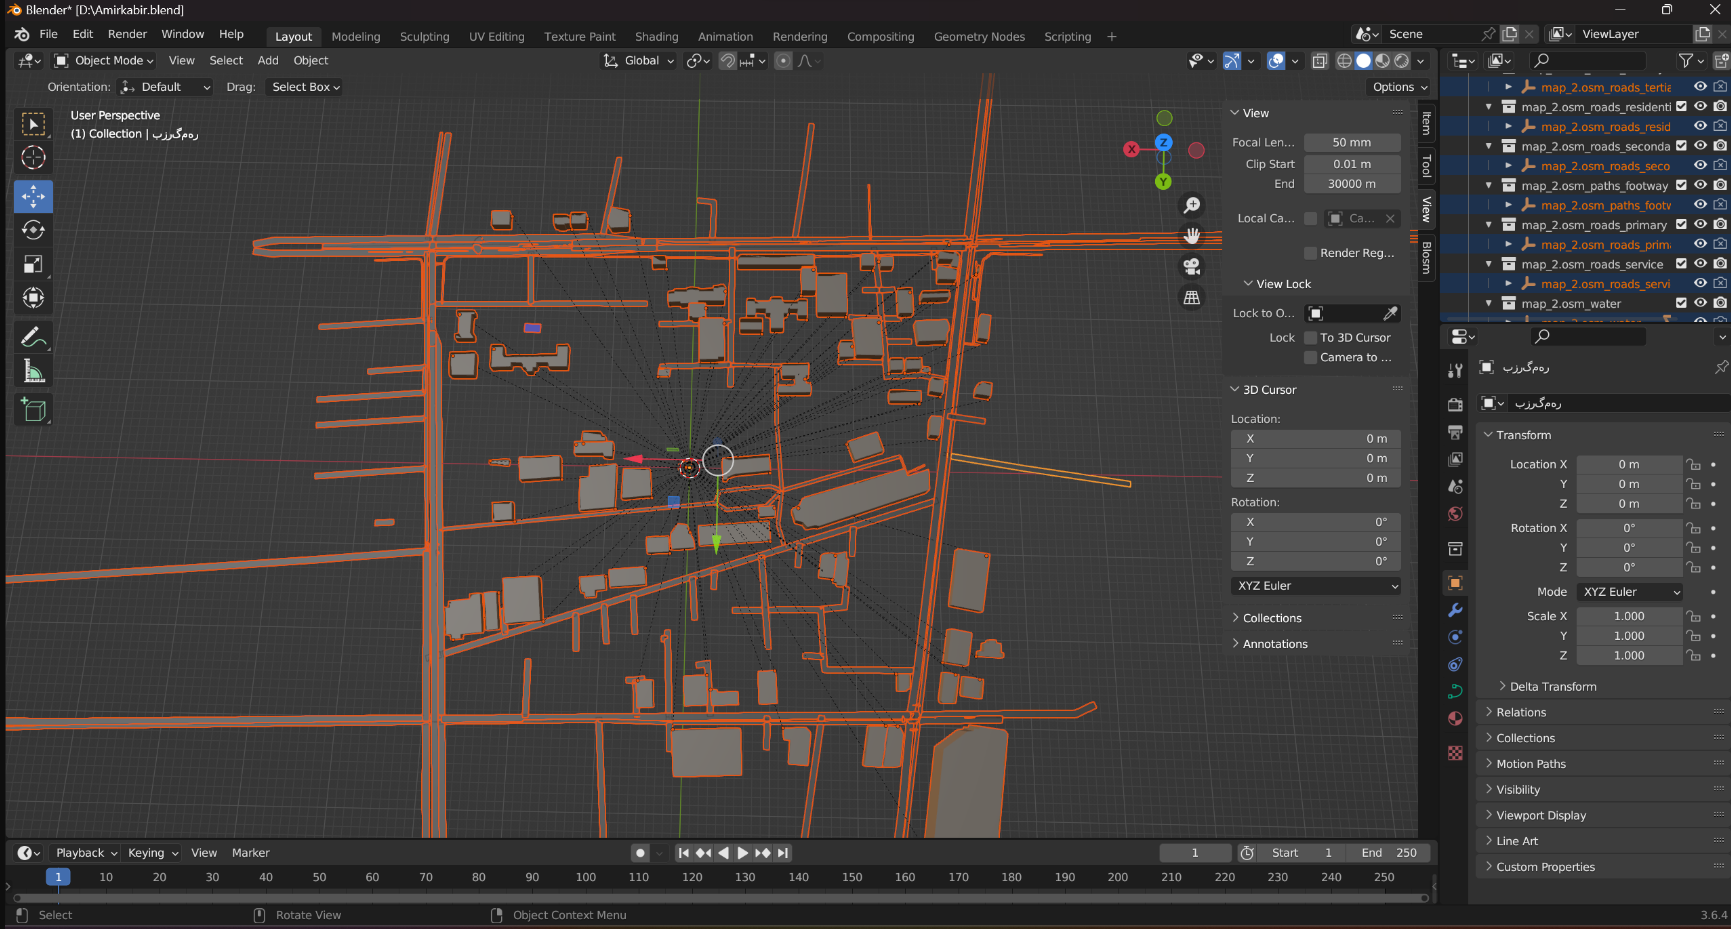
\includegraphics[width=0.9\linewidth]{figures/Amirkabir_Generated_3D_Model.png}
    \caption{مدل سه‌بعدی منطقه دانشگاه صنعتی امیرکبیر که توسط افزونه \lr{Blosm} تولید شده است.}
    \label{fig:Blosm_OSM}
\end{figure}
هر چند این مدل سه‌بعدی از منطقه امیرکبیر، \%۱۰۰ دقیق نیست؛ اما بهینه‌ترین روش برای طراحی منطقه‌ای به این بزرگی است. کار مدل‌سازی سه‌بعدی یک منطقه، کاری بسیار دشوار است و نیاز به متخصص‌هایی در این زمینه دارد. پس در این پژوهش، به همین نقشه بسنده می‌کنیم.
یکی از ویژگی‌های خوب \lr{Blender}، سازگاری آن با موتور بازی‌سازی \lr{Unity} است. این مدل را به راحتی در صحنه جدیدی که نام آن را \lr{Amirkabir\_DT\_Scene} گذاشته‌ایم، بارگذاری می‌کنیم. 
\begin{figure}[h!]
    \centering
    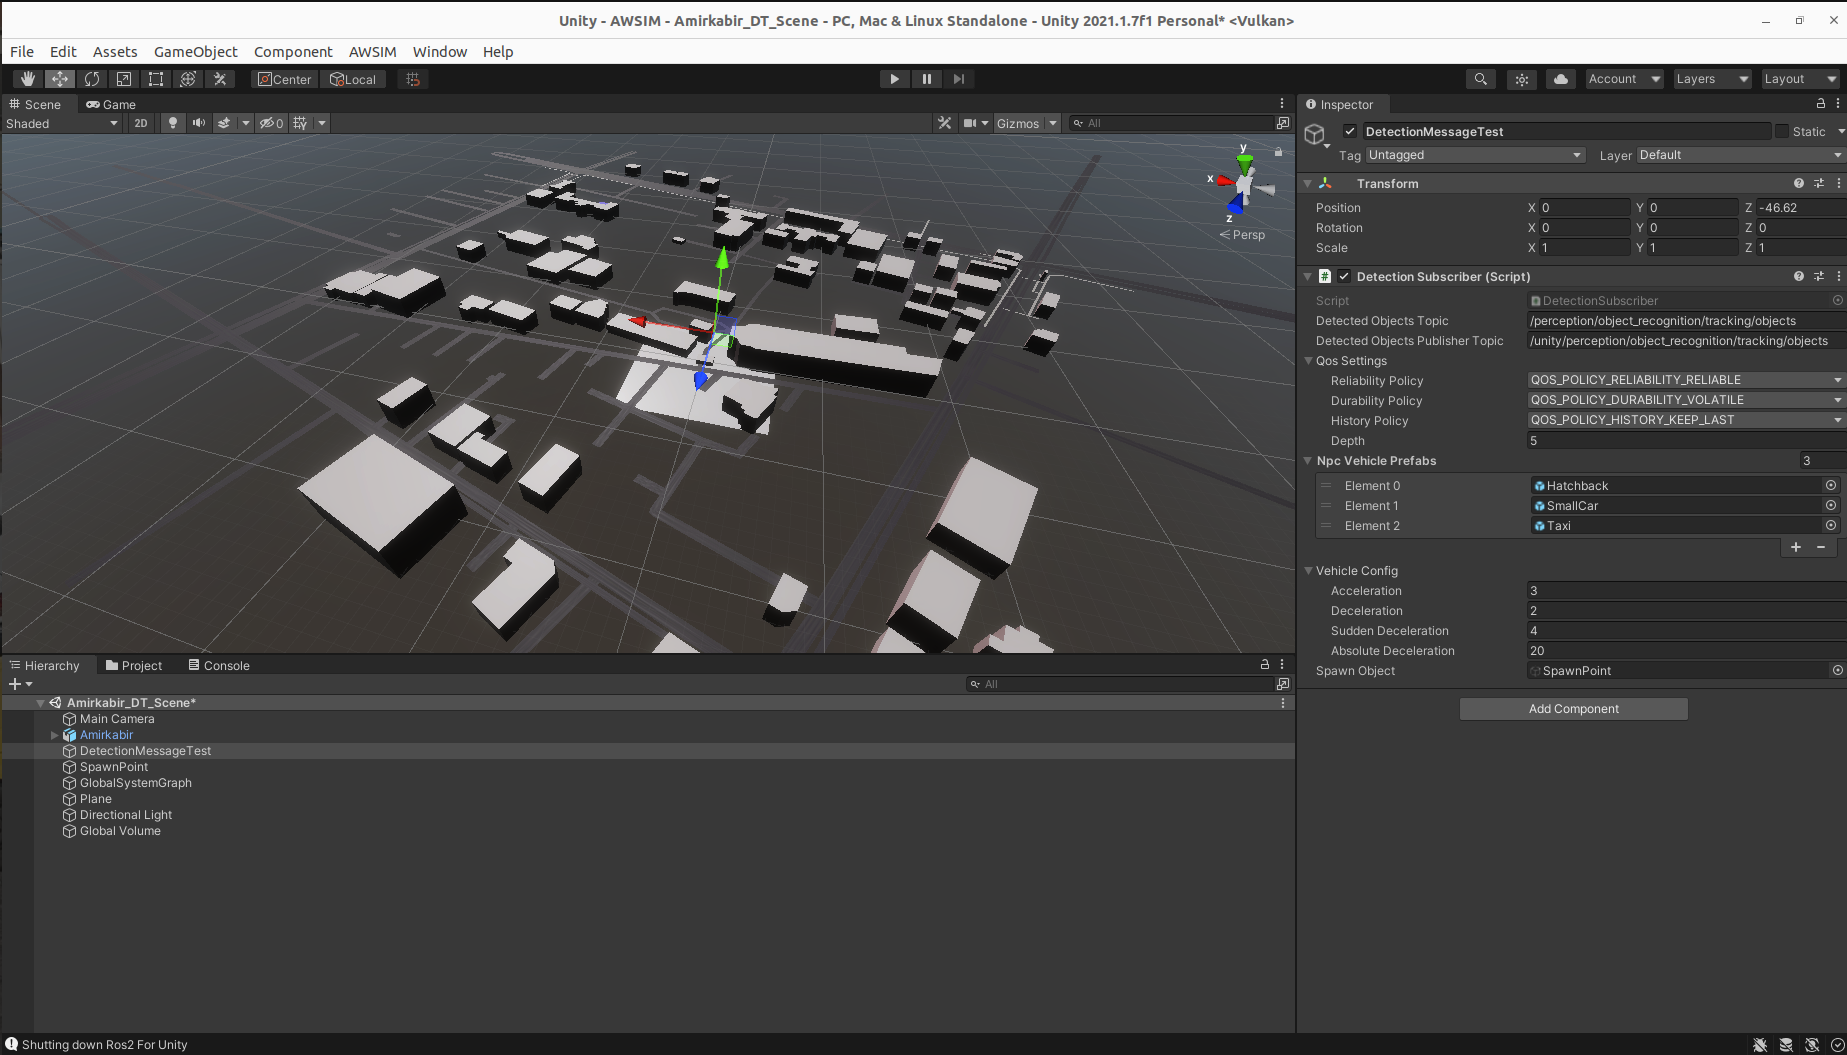
\includegraphics[width=1\linewidth]{figures/Amirkabir_Map_AWSIM.png}
    \caption{نقشه وارد شده در شبیه‌ساز \lr{AWSIM}}
    \label{fig:Amirkabir_Map_AWSIM}
\end{figure}

\section{شبیه‌سازی در خیابان رشت طراحی شده}
 روش پدیدار کردن خودروها همانند قبل است. تنها چیزی که متفاوت است،‌ مختصات شئ \lr{SpawnPoint} است. مختصات و زاویه این شئ را همانند لایداری که بالای درب رشت بود، جای گذاری می‌کنیم. بایستی دقت شود که مختصات لایدار نیز به علت ضرب شدن در ماتریس تبدیل و ماتریس دوران، تغییر کرده است.
 \begin{figure}
     \centering
     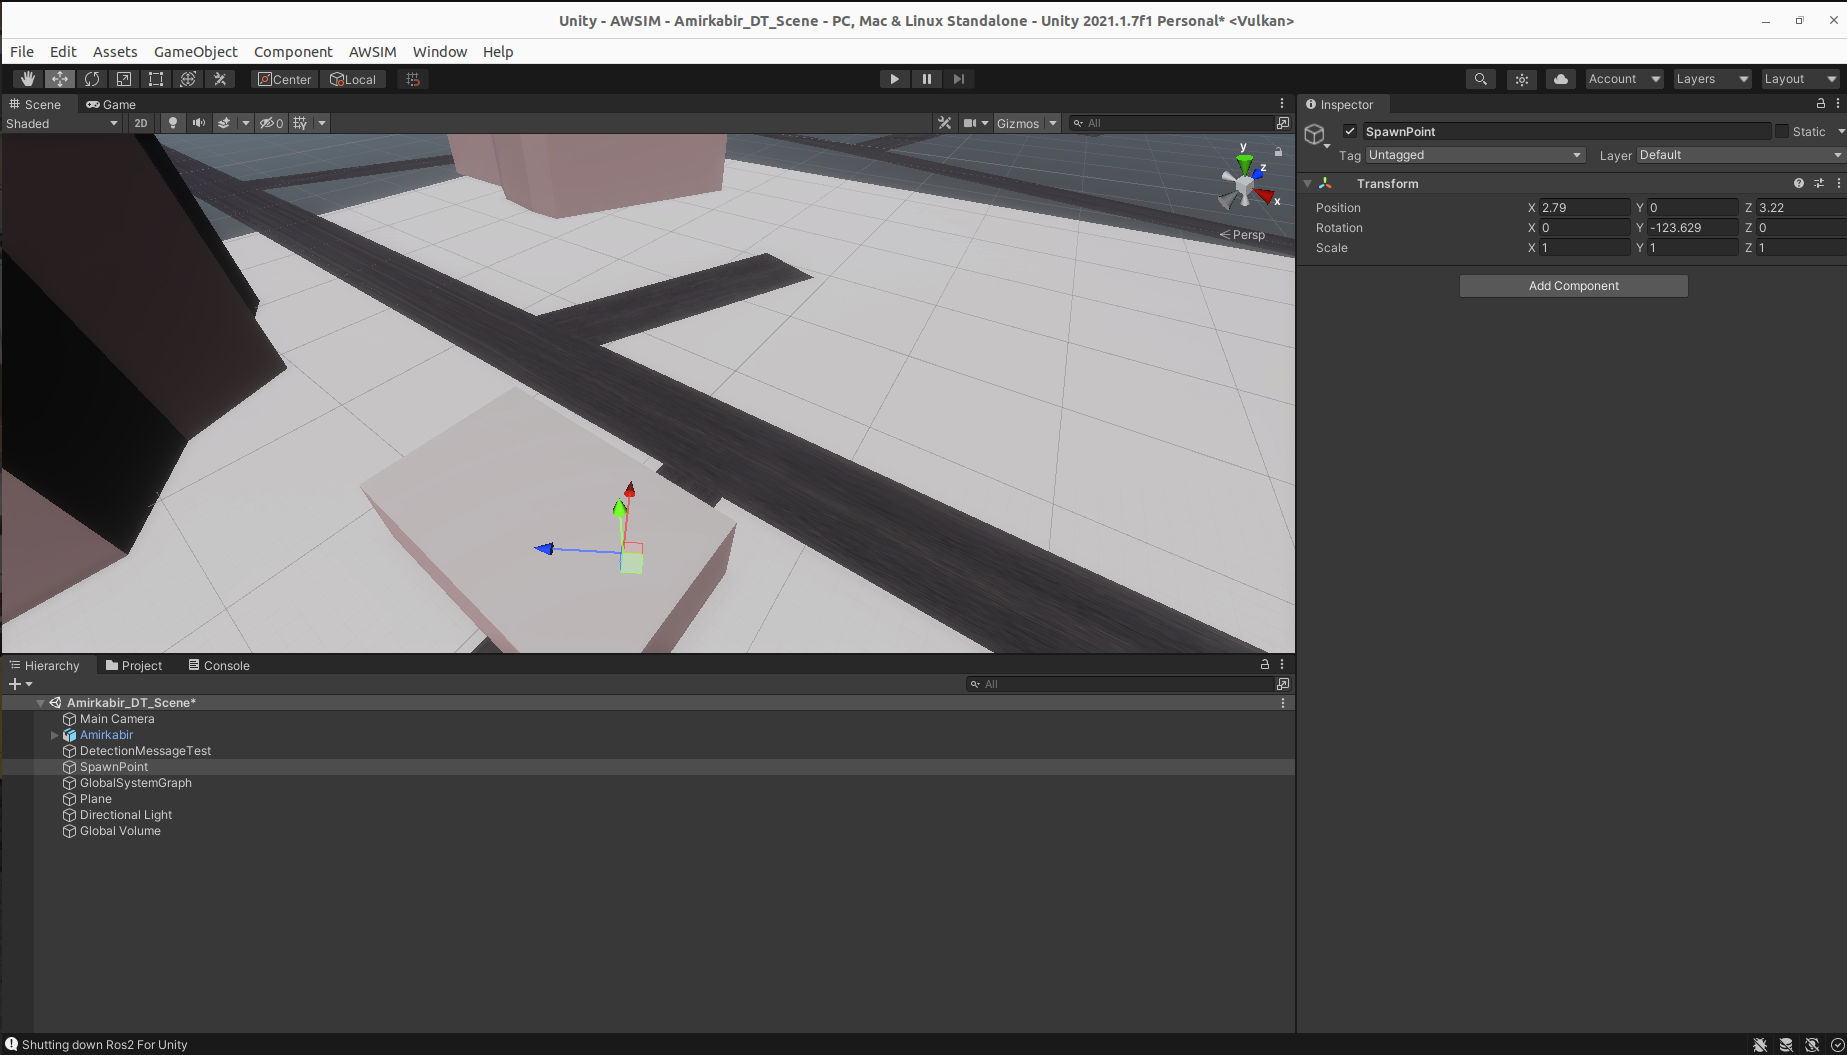
\includegraphics[width=1\linewidth]{figures/Amirkabir_DT_SpawnPoint.png}
     \caption{شئ بازی \lr{SpawnPoint} که نسبت به موقعیت تبدیل یافته لایدار مستقر شده است.}
     \label{fig:Amirkabir_DT_SpawnPoint}
 \end{figure}
 حال تبدیل‌کننده را اجرا می‌کنیم، سپس فایل‌های اجرایی دوقلوی دیجیتال ابزار \lr{Autoware} را که خود طراحی کرده‌ایم را اجرا می‌کنیم و در نهایت نیز صحنه \lr{Amirkabir\_DT\_Scene} را اجرا می‌کنیم. شکل زیر نتیجه همکاری همه‌ی پروسه‌های بخش‌های قبل، است:

 \begin{figure}[h!]
     \centering
     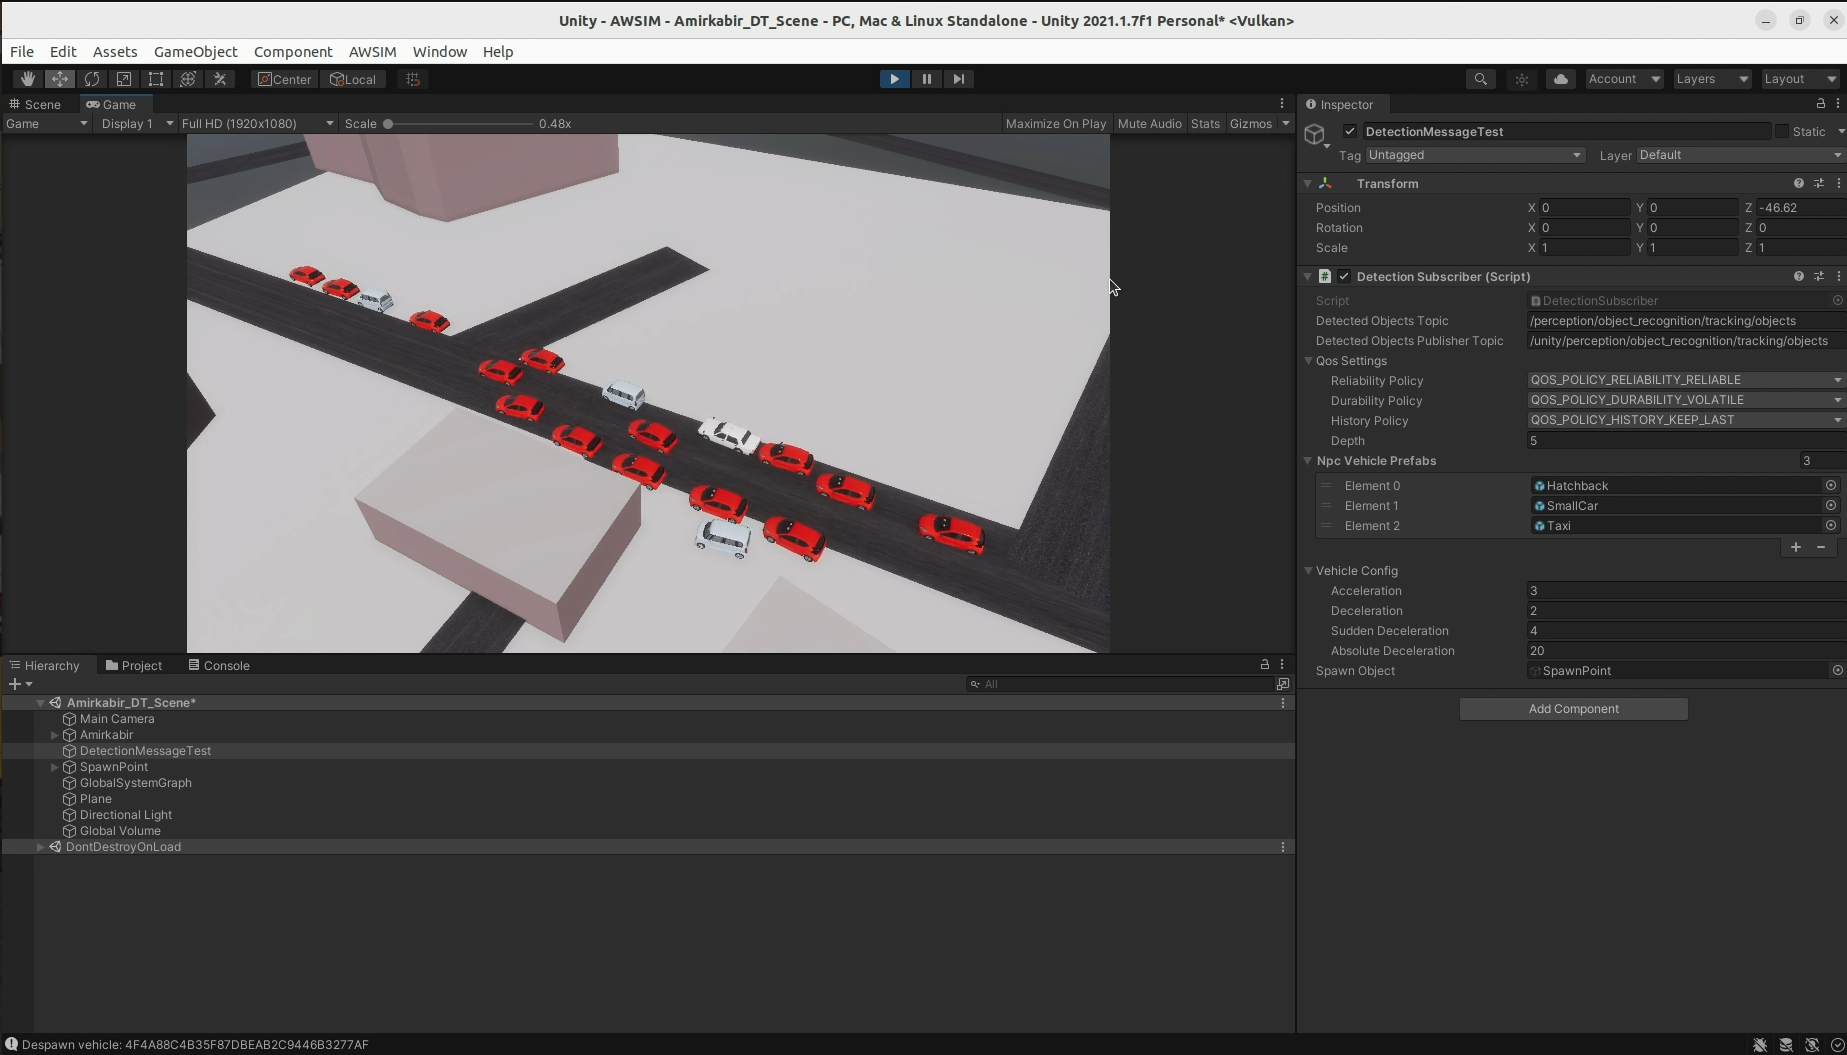
\includegraphics[width=1\linewidth]{figures/Amirkabir_Traffic_Simulation.png}
     \caption{دوقلوی تقریبی دیجیتال از خیابان رشت}
     \label{fig:Amirkabir_Traffic_Simulation}
 \end{figure}

 \begin{figure}[h!]
    \centering
    \begin{minipage}{0.8\textwidth}
        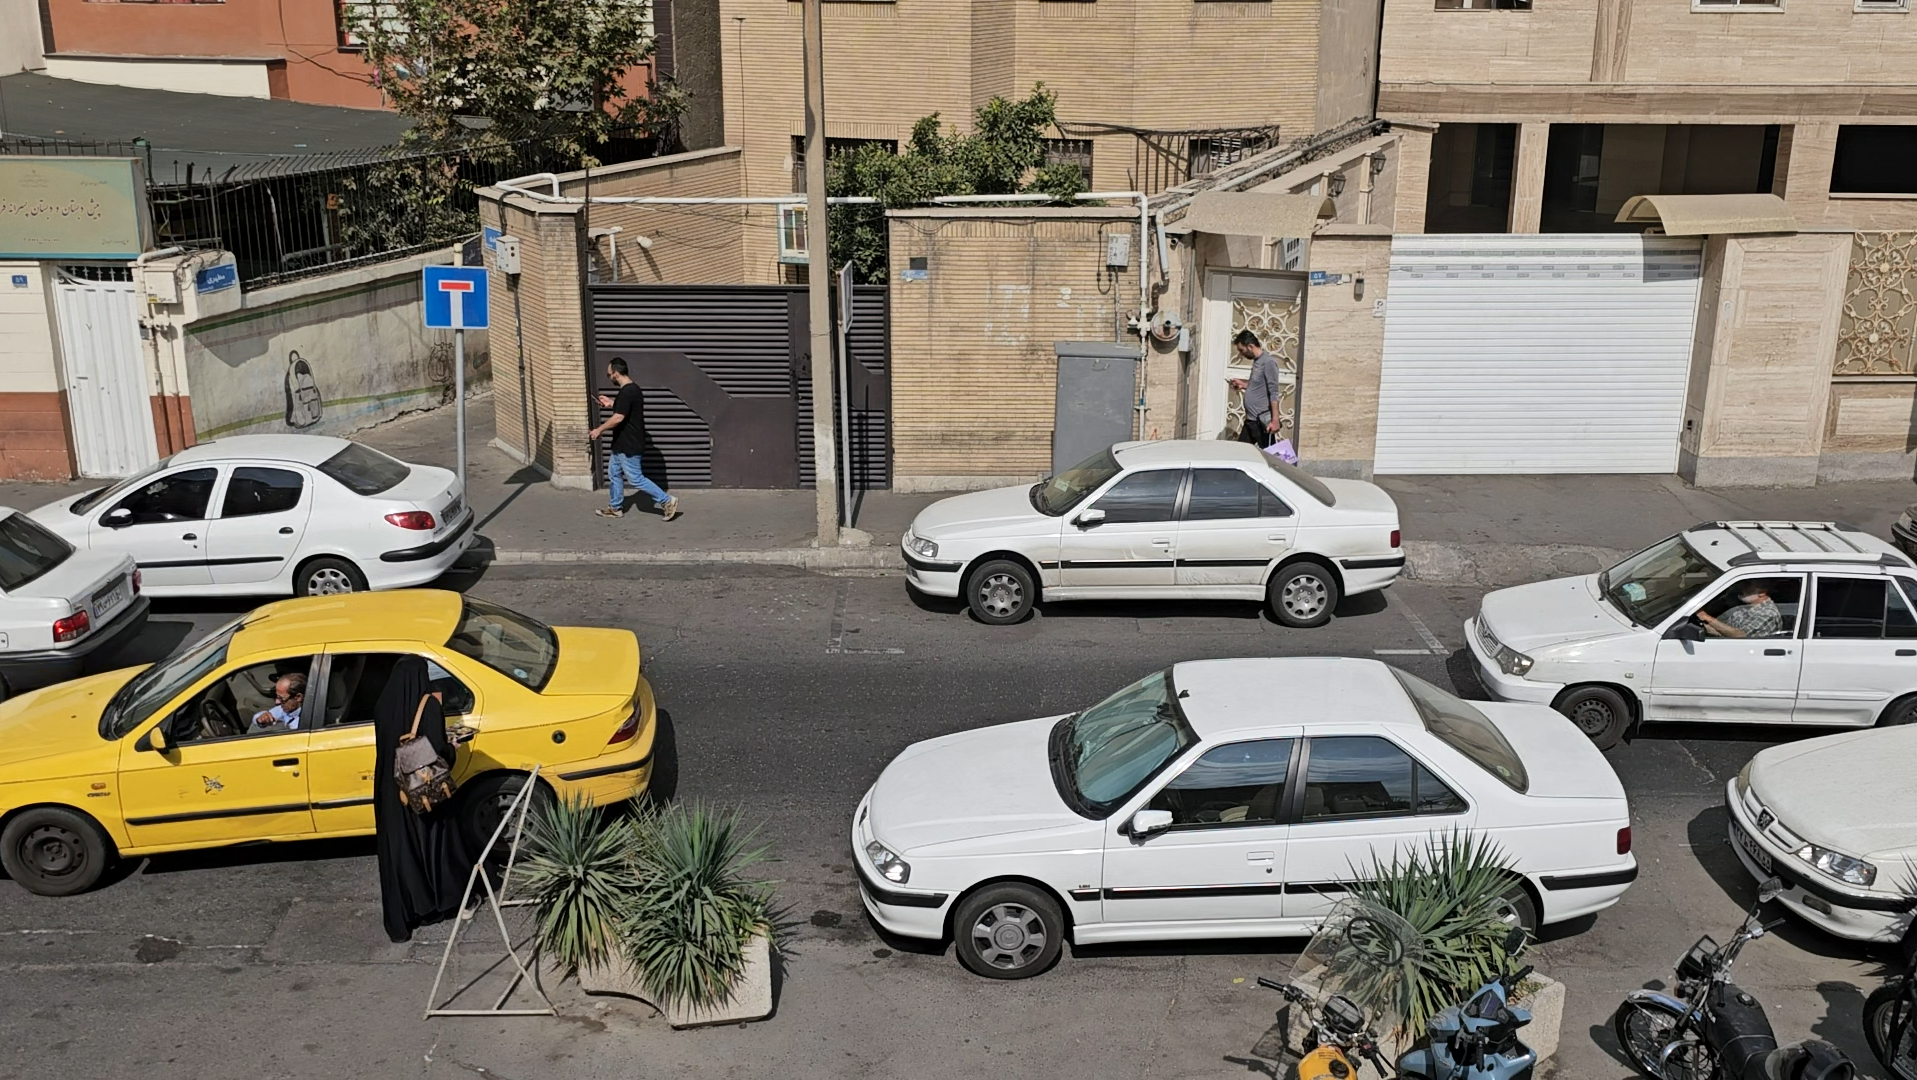
\includegraphics[width=1\linewidth]{figures/Rasht_Video_Frame_3D_Detection.png}
    \end{minipage}
    \vspace{0.3cm}
    \begin{minipage}{0.8\textwidth}
        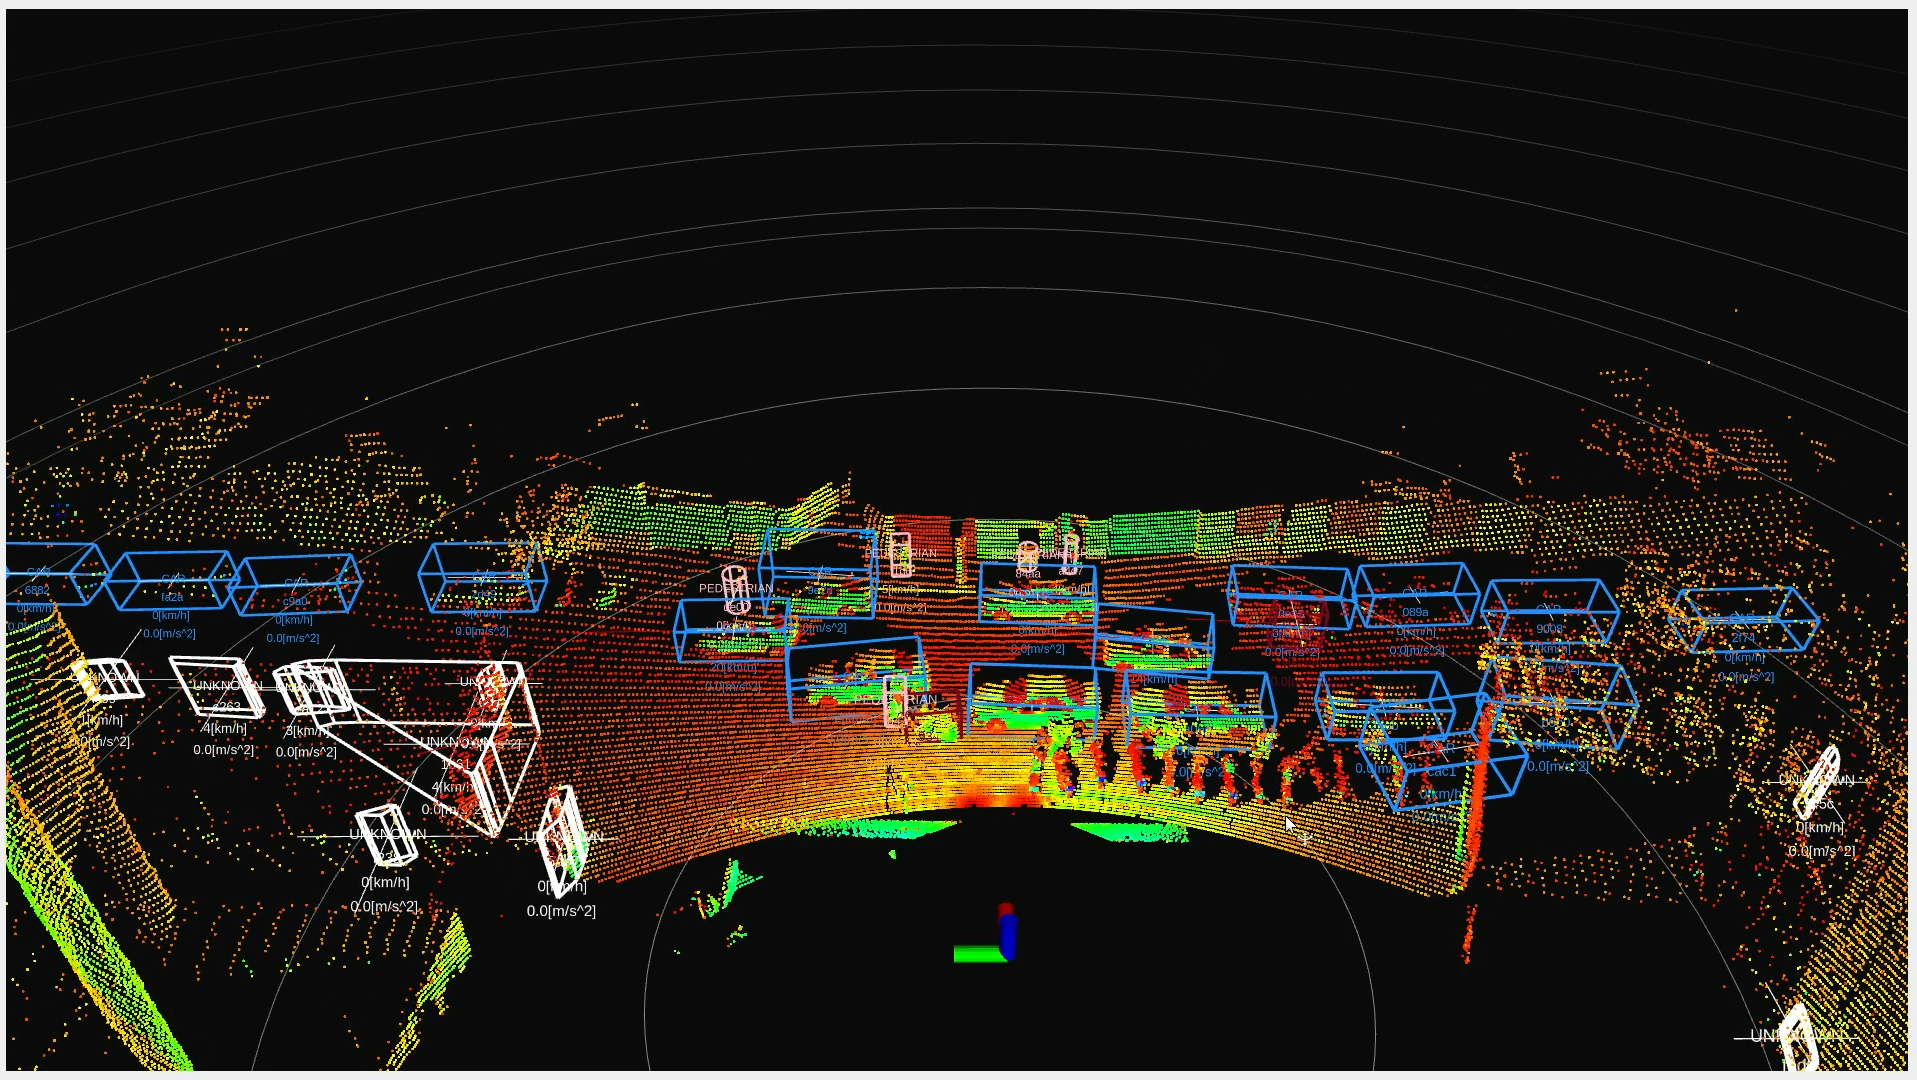
\includegraphics[width=1\linewidth]{figures/Rasht_Calibrated_3D_Detection.png}
    \end{minipage}
    \vspace{0.3cm}
    \begin{minipage}{0.8\textwidth}
        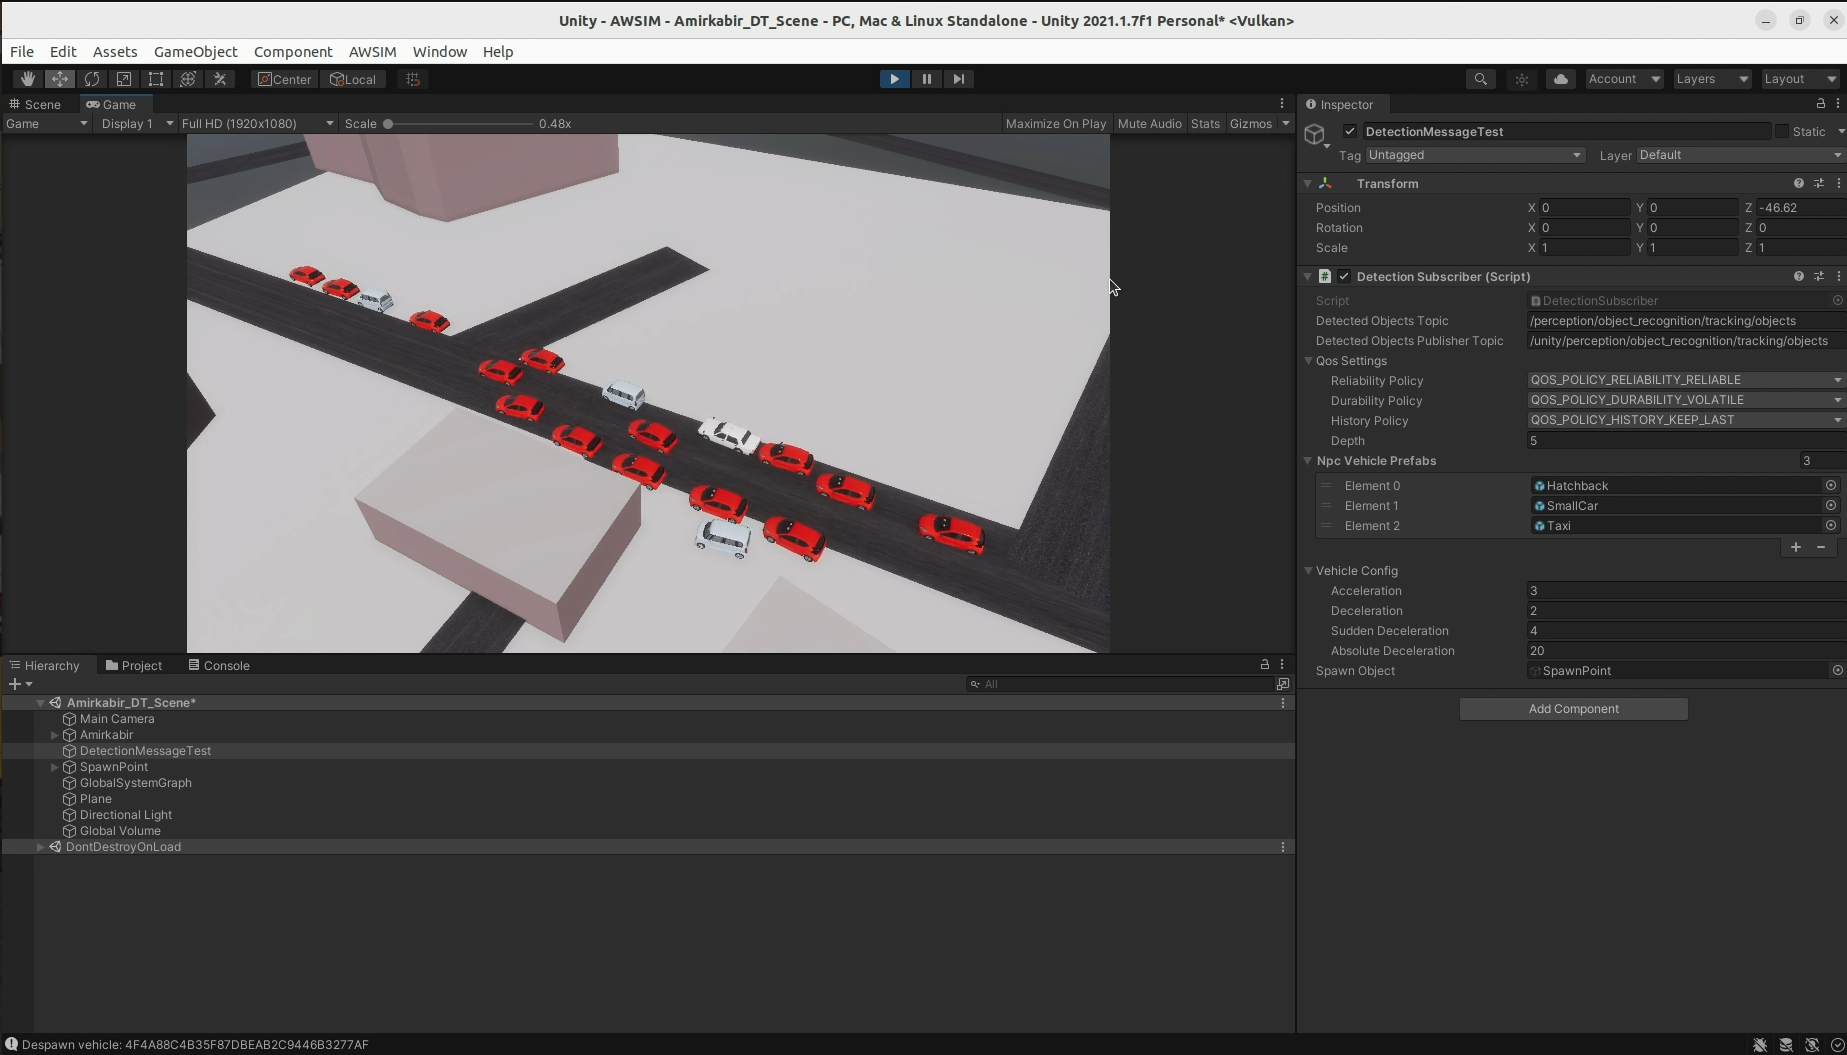
\includegraphics[width=1\linewidth]{figures/Amirkabir_Traffic_Simulation.png}
    \end{minipage}
    \caption{سه تصویر مختلف از یک لحظه زمانی (تصویر، تشخیص، شبیه‌سازی)}
    \label{fig:Digital_Twin_Frame}
\end{figure}